%% Dokumentenklasse (Koma Script) -----------------------------------------
\documentclass[%
   %draft,     % Entwurfsstadium
   final,      % fertiges Dokument
	 % --- Paper Settings ---
   paper=a4,% [Todo: add alternatives]
   paper=portrait, % landscape
   pagesize=auto, % driver
   % --- Base Font Size ---
   fontsize=11pt,%
	 % --- Koma Script Version ---
   version=last, %
 ]{scrreprt} % Classes: scrartcl, scrreprt, scrbook


% Encoding der Dateien (sonst funktionieren Umlaute nicht)
% Fuer Linux -> utf8
% Fuer Windows, alte Linux Distributionen -> latin1

% Empfohlen latin1, da einige Pakete mit utf8 Zeichen nicht
% funktionieren, z.B: listings, soul.
%\usepackage[latin1]{inputenc}
%\usepackage[ansinew]{inputenc}
\usepackage[utf8]{inputenc}
%\usepackage{ucs}
%\usepackage[utf8x]{inputenc}

%%% Preambel
%%% === Textbody ==============================================================
\KOMAoptions{%
   DIV=11,% (Size of Text Body, higher values = greater textbody)
   % DIV=calc % (also areaset/classic/current/default/last) 
   % -> after setting of spacing necessary!   
   BCOR=5mm% (Bindekorrektur)
}%
%%% === Headings ==============================================================
\KOMAoptions{%
   %%%% headings
	% headings=small,  % Small Font Size, thin spacing above and below
   % headings=normal, % Medium Font Size, medium spacing above and below
   headings=big, % Big Font Size, large spacing above and below
   %
   headings=noappendixprefix, % chapter in appendix as in body text
	headings=nochapterprefix,  % no prefix at chapters
   % headings=appendixprefix,   % inverse of 'noappendixprefix'
   % headings=chapterprefix,    % inverse of 'nochapterprefix'
   % headings=openany,   % Chapters start at any side
   % headings=openleft,  % Chapters start at left side
   headings=openright, % Chapters start at right side      
   %%% Add/Dont/Auto Dot behind section numbers 
   %%% (see DUDEN as reference)
   % numbers=autoenddot
   % numbers=enddot
   numbers=noenddot
   % secnumdepth=3 % depth of sections numbering (???)
}%
\setcounter{secnumdepth}{3}
%%% === Page Layout ===========================================================
\KOMAoptions{% (most options are for package typearea)
   twoside=true, % two side layout (alternating margins, standard in books)
   % twoside=false, % single side layout 
   % twoside=semi,  % two side layout (non alternating margins!)
   %
   twocolumn=false, % (true)
   %
   headinclude=false,%
   footinclude=false,%
   mpinclude=false,%      
   %
   headlines=2.1,%
	% headheight=2em,%
   headsepline=true,%
   footsepline=false,%
   cleardoublepage=empty %plain, headings
}%
%%% === Paragraph Separation ==================================================
\KOMAoptions{%
	% parskip=relative, % change indentation according to fontsize (recommanded)
   parskip=absolute, % do not change indentation according to fontsize
   parskip=false    % indentation of 1em
   % parskip=true   % parksip of 1 line - with free space in last line of 1em
   % parskip=full-  % parksip of 1 line - no adjustment
   % parskip=full+  % parksip of 1 line - with free space in last line of 1/4
   % parskip=full*  % parksip of 1 line - with free space in last line of 1/3
   % parskip=half   % parksip of 1/2 line - with free space in last line of 1em
   % parskip=half-  % parksip of 1/2 line - no adjustment
   % parskip=half+  % parksip of 1/2 line - with free space in last line of 1/3
   % parskip=half*  % parksip of 1/2 line - with free space in last line of 1em
}%
%%% === Table of Contents =====================================================
\setcounter{tocdepth}{3} % Depth of TOC Display
\KOMAoptions{%
   %%% Setting of 'Style' and 'Content' of TOC
   % toc=left, %
   toc=indented,%
   %
   toc=bib,
   % toc=nobib,
   % toc=bibnumbered,
   %
	% toc=index,%
   toc=noindex,
   %
   % toc=listof,
   toc=nolistof
   % toc=listofnumbered,
   %   
}%  
%%% === Lists of figures, tables etc. =========================================
\KOMAoptions{%
   %%% Setting of 'Style' and 'Content' of Lists 
   %%% (figures, tables etc)
	% --- General List Style ---
   listof=left, % tabular styles
   listof=indented, % hierarchical style
   % --- chapter highlighting ---
   % listof=chapterentry, % ??? Chapter starts are marked in figure/table
   % listof=chaptergapline, % New chapter starts are marked by a gap 
      		  			   	 % of a single line
	listof=chaptergapsmall, % New chapter starts are marked by a gap 
   	    					   % of a smallsingle line
   % listof=nochaptergap, % No Gap between chapters
   %
   % listof=leveldown, % lists are moved one level down ???
   % --- Appearance of Lists in TOC
   % listof=notoc, % Lists are not part of the TOC
   listof=totoc % add Lists to TOC without number
   % listof=totocnumbered, % add Lists to TOC with number
}%  
%%% === Bibliography ==========================================================
%% Setting of 'Style' and 'Content' of Bibliography
\KOMAoptions{%
	% bibliography=oldstyle,%
   bibliography=openstyle,%
   % bibliography=nottotoc, % Bibliography is not part of the TOC
   % bibliography=totocnumbered, % add Bibliography to TOC with number
   bibliography=totoc % add Bibliography to TOC without number
}%
%%% === Index =================================================================
%% Setting of 'Style' and 'Content' of Index in TOC
\KOMAoptions{%
   index=nottotoc % index is not part of the TOC
	% index=totoc, % add index to TOC without number
}%
%%% === Titlepage =============================================================
\KOMAoptions{%
   titlepage=true %
   %titlepage=false %
}%
%%% === Miscellaneous =========================================================
\KOMAoptions{% 	
   footnotes=multiple% nomultiple
   %open=any,%
   %open=left,%
   %open=right,%
   %chapterprefix=false,%
   %appendixprefix=false,%
   %chapteratlists=10pt,% entry
}%
% ------------------------------------------------------------------------
% LaTeX - Preambel  ******************************************************
% ------------------------------------------------------------------------
% von: Matthias Pospiech
% ========================================================================

% Strukturierung dieser Praeambel:
%    1.  Pakete die vor anderen geladen werden müssen
%        (calc, babel, xcolor, graphicx, amsmath, pst-pdf, ragged2e, ...)
%    2.  Schriften
%    3.  Mathematik (mathtools, fixmath, onlyamsmath, braket,
%        cancel, empheq, exscale, icomma, ...)
%    4.  Tabellen (booktabs, multirow, dcolumn, tabularx, ltxtable, supertabular)
%    5.  Text
%        5.1 Auszeichnungen (ulem, soul, url)
%        5.2 Fussnoten (footmisc)
%        5.3 Verweise (varioref)
%        5.4 Listen (enumitem, paralist, declist)
%    6.  Zitieren (csquotes, jurabib, natbib)
%    7.  PDF (microtype, hyperref, backref, hypcap, pdfpages
%    8.  Graphiken (float, flafter, placeins, subfig, wrapfig,
%        floatflt, picins, psfrag, sidecap, pict2e, curve2e)
%    9.  Sonstiges (makeidx, isodate, numprint, nomencl, acronym)
%    10. Verbatim (upquote, verbatim, fancyvrb, listings, examplep)
%    11. Wissenschaft (units)
%    12. Fancy Stuff
%    13. Layout
%       13.1.  Diverse Pakete und Einstellungen (multicol, ellipsis)
%       13.2.  Zeilenabstand (setspace)
%       13.3.  Seitenlayout (typearea, geometry)
%       13.4.  Farben
%       13.5.  Aussehen der URLS
%       13.6.  Kopf und Fusszeilen (scrlayer-scrpage)
%       13.7.  Fussnoten
%       13.8.  Schriften (Sections )
%       13.9.  UeberSchriften (Chapter und Sections) (titlesec, indentfirst)
%       13.10. Captions (Schrift, Aussehen)
%              (caption, subfig, capt-of, mcaption, tocloft, multitoc, minitoc)
%    14.  Auszufuehrende Befehle
%    15. DoDo Notes Package


% ~~~~~~~~~~~~~~~~~~~~~~~~~~~~~~~~~~~~~~~~~~~~~~~~~~~~~~~~~~~~~~~~~~~~~~~~
% Einige Pakete muessen unbedingt vor allen anderen geladen werden
% ~~~~~~~~~~~~~~~~~~~~~~~~~~~~~~~~~~~~~~~~~~~~~~~~~~~~~~~~~~~~~~~~~~~~~~~~

%%% Packages for LaTeX - programming
%
% Define commands that don't eat spaces.
\usepackage{xspace}
% IfThenElse
\usepackage{ifthen}
%%% Doc: ftp://tug.ctan.org/pub/tex-archive/macros/latex/contrib/oberdiek/ifpdf.sty
% command for testing for pdf-creation
\usepackage{ifpdf} %\ifpdf \else \fi

%%% Internal Commands: ----------------------------------------------
\makeatletter
%
\providecommand{\IfPackageLoaded}[2]{\@ifpackageloaded{#1}{#2}{}}
\providecommand{\IfPackageNotLoaded}[2]{\@ifpackageloaded{#1}{}{#2}}
\providecommand{\IfElsePackageLoaded}[3]{\@ifpackageloaded{#1}{#2}{#3}}
%
\newboolean{chapteravailable}%
\setboolean{chapteravailable}{false}%

\ifcsname chapter\endcsname
  \setboolean{chapteravailable}{true}%
\else
  \setboolean{chapteravailable}{false}%
\fi


\providecommand{\IfChapterDefined}[1]{\ifthenelse{\boolean{chapteravailable}}{#1}{}}%
\providecommand{\IfElseChapterDefined}[2]{\ifthenelse{\boolean{chapteravailable}}{#1}{#2}}%

\providecommand{\IfDefined}[2]{%
\ifcsname #1\endcsname
   #2 %
\else
     % do nothing
\fi
}

\providecommand{\IfElseDefined}[3]{%
\ifcsname #1\endcsname
   #2 %
\else
   #3 %
\fi
}

\providecommand{\IfElseUnDefined}[3]{%
\ifcsname #1\endcsname
   #3 %
\else
   #2 %
\fi
}


%
% Check for 'draft' mode - commands.
\newcommand{\IfNotDraft}[1]{\ifx\@draft\@undefined #1 \fi}
\newcommand{\IfNotDraftElse}[2]{\ifx\@draft\@undefined #1 \else #2 \fi}
\newcommand{\IfDraft}[1]{\ifx\@draft\@undefined \else #1 \fi}
%

% Definde frontmatter, mainmatter and backmatter if not defined
\@ifundefined{frontmatter}{%
   \newcommand{\frontmatter}{%
      %In Roemischen Buchstaben nummerieren (i, ii, iii)
      \pagenumbering{roman}
   }
}{}
\@ifundefined{mainmatter}{%
   % scrpage2 benoetigt den folgenden switch
   % wenn \mainmatter definiert ist.
   \newif\if@mainmatter\@mainmattertrue
   \newcommand{\mainmatter}{%
      % -- Seitennummerierung auf Arabische Zahlen zuruecksetzen (1,2,3)
      \pagenumbering{arabic}%
      \setcounter{page}{1}%
   }
}{}
\@ifundefined{backmatter}{%
   \newcommand{\backmatter}{
      %In Roemischen Buchstaben nummerieren (i, ii, iii)
      \pagenumbering{roman}
   }
}{}

% Pakete speichern die spaeter geladen werden sollen
\newcommand{\LoadPackagesNow}{}
\newcommand{\LoadPackageLater}[1]{%
   \g@addto@macro{\LoadPackagesNow}{%
      \usepackage{#1}%
   }%
}



\makeatother
%%% ----------------------------------------------------------------
%
%%% Doc: www.cs.brown.edu/system/software/latex/doc/calc.pdf
% Calculation with LaTeX
\usepackage{calc}

%%% Doc: ftp://tug.ctan.org/pub/tex-archive/macros/latex/required/babel/babel.pdf
% Languagesetting
\usepackage[
%	german,
	ngerman,
%	english,
%	french,
]{babel}

%%% Doc: ftp://tug.ctan.org/pub/tex-archive/macros/latex/contrib/xcolor/xcolor.pdf
% Farben
% Incompatible: Do not load when using pstricks !
\usepackage[
	table % Load for using rowcolors command in tables
]{xcolor}


%%% Doc: ftp://tug.ctan.org/pub/tex-archive/macros/latex/required/graphics/grfguide.pdf
% Bilder
\usepackage[%
	%final,
	%draft % do not include images (faster)
]{graphicx}

%%% Doc: ftp://tug.ctan.org/pub/tex-archive/macros/latex/contrib/oberdiek/epstopdf.pdf
%% If an eps image is detected, epstopdf is automatically called to convert it to pdf format.
%% Requires: graphicx loaded
\usepackage{epstopdf}

\usepackage{hyperref}

%%% Doc: ftp://tug.ctan.org/pub/tex-archive/macros/latex/required/amslatex/math/amsldoc.pdf
% Amsmath - Mathematik Basispaket
%
% fuer pst-pdf displaymath Modus vor pst-pdf benoetigt.
\usepackage[
   centertags, % (default) center tags vertically
   %tbtags,    % 'Top-or-bottom tags': For a split equation, place equation numbers level
               % with the last (resp. first) line, if numbers are on the right (resp. left).
   sumlimits,  %(default) Place the subscripts and superscripts of summation
               % symbols above and below
   %nosumlimits, % Always place the subscripts and superscripts of summation-type
               % symbols to the side, even in displayed equations.
   intlimits,  % Like sumlimits, but for integral symbols.
   %nointlimits, % (default) Opposite of intlimits.
   namelimits, % (default) Like sumlimits, but for certain 'operator names' such as
               % det, inf, lim, max, min, that traditionally have subscripts placed underneath
               % when they occur in a displayed equation.
   %nonamelimits, % Opposite of namelimits.
   %leqno,     % Place equation numbers on the left.
   %reqno,     % Place equation numbers on the right.
   fleqn,     % Position equations at a fixed indent from the left margin
   			  % rather than centered in the text column.
]{amsmath} %
% eqnarray nicht zusammen mit amsmath benutzen, siehe l2tabu.pdf für
% Hintergruende.

%%% Doc: http://www.ctan.org/tex-archive/macros/latex/contrib/pst-pdf/pst-pdf-DE.pdf
% Used to automatically integrate eps graphics in an pdf document using pdflatex.
% Requires ps4pdf macro !!!
% Download macro from http://www.ctan.org/tex-archive/macros/latex/contrib/pst-pdf/scripts/
%
%\usepackage[%
%   %active,       % Aktiviert den Extraktionsmodus (DVI-Ausgabe). Die explizite Angabe ist
%                  % normalerweise unnötig (Standard im LATEX-Modus).
%   %inactive,     % Das Paket wird deaktiviert, Zuätzlich werden die Pakete pstricks und
%                  % graphicx geladen
%   nopstricks,    % Das Paket pstricks wird nicht geladen.
%   %draft,        % Im pdfLATEX-Modus werden aus der Containerdatei eingefügte Grafiken nur
%                  % als Rahmen dargestellt.
%   %final,        % Im pdfLATEX-Modus werden aus der Containerdatei eingefügte Grafiken
%                  % vollständig dargestellt (Standard).
%   %tightpage,    % Die Abmessung Grafiken in der Containerdatei entsprechen denen der
%                  % zugehörigen TEX-Boxen (Standard).
%   %notightpage,  % die Grafiken in der Containerdatei nehmen
%                  % mindestens die Größe des gesamten Blattes einnehmen.
%   %displaymath,  % Es werden zusätzlich die mathematischen Umgebungen displaymath,
%                  % eqnarray und $$ extrahiert und im pdf-Modus als Grafik eingefügt.
%]{pst-pdf}
%
% Notwendiger Bugfix für natbib Paket bei Benutzung von pst-pdf (Version <= v1.1o)
\IfPackageLoaded{pst-pdf}{
   \providecommand\makeindex{}
   \providecommand\makeglossary{}
}{}

%% Doc: ftp://tug.ctan.org/pub/tex-archive/graphics/pstricks/README
% load before graphicx
% \usepackage{pstricks}
% \usepackage{pst-plot, pst-node, pst-coil, pst-eps}

% This package implements a workaround for the LaTeX bug that marginpars
% sometimes appear on the wrong margin.
% \usepackage{mparhack}
% in some case this causes an error in the index together with package pdfpages
% the reason is unkown. Therefore I recommend to use the margins of marginnote

%% Doc: ftp://tug.ctan.org/pub/tex-archive/macros/latex/contrib/marginnote/marginnote.pdf
% Summary description: marginnote allows margin note, where \marginpar fails
\usepackage{marginnote}


%% Doc: (inside relsize.sty )
%% ftp://tug.ctan.org/pub/tex-archive/macros/latex/contrib/misc/relsize.sty
%  Set the font size relative to the current font size
\usepackage{relsize}

%% Doc: ftp://tug.ctan.org/pub/tex-archive/macros/latex/contrib/ms/ragged2e.pdf
% Besserer Flatternsatz (Linksbuendig, statt Blocksatz)
\usepackage{ragged2e}

% ~~~~~~~~~~~~~~~~~~~~~~~~~~~~~~~~~~~~~~~~~~~~~~~~~~~~~~~~~~~~~~~~~~~~~~~~
% Fonts Fonts Fonts
% ~~~~~~~~~~~~~~~~~~~~~~~~~~~~~~~~~~~~~~~~~~~~~~~~~~~~~~~~~~~~~~~~~~~~~~~~

\usepackage[T1]{fontenc} % T1 Schrift Encoding
\usepackage{textcomp}	 % Zusatzliche Symbole (Text Companion font extension)

%%% Schriften werden in Fonts.tex geladen
% ~~~~~~~~~~~~~~~~~~~~~~~~~~~~~~~~~~~~~~~~~~~~~~~~~~~~~~~~~~~~~~~~~~~~~~~~
% Fonts Fonts Fonts
% ~~~~~~~~~~~~~~~~~~~~~~~~~~~~~~~~~~~~~~~~~~~~~~~~~~~~~~~~~~~~~~~~~~~~~~~~

% Alle Schriften die hier angegeben sind sehen im PDF richtig aus.
% Die LaTeX Standardschrift ist die Latin Modern (lmodern Paket).
% If Latin Modern is not available for your distribution you must install the
% package cm-super instead. Otherwise your fonts will look horrible in the PDF

% DO NOT LOAD ae Package for the font !

%% ==== Zusammengesetzte Schriften  (Sans + Serif) =======================

%% - Latin Modern
\usepackage{lmodern}
%% -------------------
%
%% - Times, Helvetica, Courier (Word Standard...)
%\usepackage{mathptmx}
%\usepackage[scaled=.90]{helvet}
%\usepackage{courier}
%% -------------------
%%
%% - Palantino , Helvetica, Courier
%\usepackage{mathpazo}
%\usepackage[scaled=.95]{helvet}
%\usepackage{courier}
%% -------------------
%
%% - Bera Schriften
%\usepackage{bera}
%% -------------------
%
%% - Charter, Bera Sans
%\usepackage{charter}\linespread{1.05}
%\renewcommand{\sfdefault}{fvs}

%% ===== Serifen =========================================================

%\usepackage{mathpazo}                 %% --- Palantino
%\usepackage{charter}\linespread{1.05} %% --- Charter
%\usepackage{bookman}                  %% --- Bookman (laedt Avant Garde !!)
%\usepackage{newcent}                  %% --- New Century Schoolbook (laedt Avant Garde !!)

%\usepackage[%                         %% --- Fourier
%   upright,     % Math fonts are upright
%   expert,      % Only for EXPERT Fonts!
%   oldstyle,    % Only for EXPERT Fonts!
%   fulloldstyle % Only for EXPERT Fonts!
%]{fourier} %



%% ===== Sans Serif ======================================================

%\usepackage[scaled=.95]{helvet}        %% --- Helvetica
%\usepackage{cmbright}                  %% --- CM-Bright (eigntlich eine Familie)
%\usepackage{tpslifonts}                %% --- tpslifonts % Font for Slides
%\usepackage{avantgar}                  %% --- Avantgarde

%%%% =========== Italics ================

%\usepackage{chancery}                  %% --- Zapf Chancery

%%%% =========== Typewriter =============

%\usepackage{courier}                   %% --- Courier
%\renewcommand{\ttdefault}{cmtl}        %% --- CmBright Typewriter Font
%\usepackage[%                          %% --- Luxi Mono (Typewriter)
%   scaled=0.9
%]{luximono}



%%%% =========== Mathe ================

%% Recommanded to use with fonts: Aldus, Garamond, Melior, Sabon
%\usepackage[                           %% --- EulerVM (MATH)
%   small,       %for smaller Fonts
%  euler-digits % digits in euler fonts style
%]{eulervm}

% \usepackage[
% %   utopia,
% %   garamond,
%    charter
% ]{mathdesign}

%%%% (((( !!! kommerzielle Schriften !!! )))))))))))))))))))))))))))))))))))))))))))))))))))

%% ===== Serifen (kommerzielle Schriften ) ================================

%% --- Adobe Aldus
%\renewcommand{\rmdefault}{pasx}
%\renewcommand{\rmdefault}{pasj} %%oldstyle digits
% math recommended: \usepackage[small]{eulervm}

%% --- Adobe Garamond
%\usepackage[%
%   osf,        % oldstyle digits
%   scaled=1.05 %appropriate in many cases
%]{xagaramon}
% math recommended: \usepackage{eulervm}

%% --- Adobe Stempel Garamond
%\renewcommand{\rmdefault}{pegx}
%\renewcommand{\rmdefault}{pegj} %%oldstyle digits

%% --- Adobe Melior
%\renewcommand{\rmdefault}{pml}
% math recommended: %\usepackage{eulervm}

%% --- Adobe Minion
%\renewcommand{\rmdefault}{pmnx}
%\renewcommand{\rmdefault}{pmnj} %oldstyle digits
% math recommended: \usepackage[small]{eulervm} or \usepackage{mathpmnt} % commercial

%% --- Adobe Sabon
%\renewcommand{\rmdefault}{psbx}
%\renewcommand{\rmdefault}{psbj} %oldstyle digits
% math recommended: \usepackage{eulervm}

%% --- Adobe Times
% math recommended: \usepackage{mathptmx} % load first !
%\renewcommand{\rmdefault}{ptmx}
%\renewcommand{\rmdefault}{ptmj} %oldstyle digits

%% --- Linotype ITC Charter
%\renewcommand{\rmdefault}{lch}

%% --- Linotype Meridien
%\renewcommand{\rmdefault}{lmd}

%%% ===== Sans Serif (kommerzielle Schriften) ============================

%% --- Adobe Frutiger
%\usepackage[
%   scaled=0.90
%]{frutiger}

%% --- Adobe Futura (=Linotype FuturaLT) : Sans Serif
%\usepackage[
%   scaled=0.94  % appropriate in many cases
%]{futura}

%% --- Adobe Gill Sans : Sans Serif
%\usepackage{gillsans}

%% -- Adobe Myriad  : Sans Serif
%\renewcommand{\sfdefault}{pmy}
%\renewcommand{\sfdefault}{pmyc} %% condensed Font

%% --- Syntax : sans serif font
%\usepackage[
%   scaled
%]{asyntax}

%% --- Adobe Optima : Semi Sans Serif
%\usepackage[
%   medium %darker medium weight fonts
%]{optima}

%% --- Linotype ITC Officina Sans
%\renewcommand{\sfdefault}{lo9}





% ~~~~~~~~~~~~~~~~~~~~~~~~~~~~~~~~~~~~~~~~~~~~~~~~~~~~~~~~~~~~~~~~~~~~~~~~
% Math Packages
% ~~~~~~~~~~~~~~~~~~~~~~~~~~~~~~~~~~~~~~~~~~~~~~~~~~~~~~~~~~~~~~~~~~~~~~~~

% *** Mathematik **************************************
%
% amsmath schon vorher geladen da es vor pst-pdf geladen werden muss


%%% Doc: ftp://tug.ctan.org/pub/tex-archive/macros/latex/contrib/mh/doc/mathtools.pdf
% Erweitert amsmath und behebt einige Bugs
\usepackage[fixamsmath,disallowspaces]{mathtools}

%%% Doc: http://www.ctan.org/info?id=fixmath
% LaTeX's default style of typesetting mathematics does not comply
% with the International Standards ISO31-0:1992 to ISO31-13:1992
% which indicate that uppercase Greek letters always be typset
% upright, as opposed to italic (even though they usually
% represent variables) and allow for typsetting of variables in a
% boldface italic style (even though the required fonts are
% available). This package ensures that uppercase Greek be typeset
% in italic style, that upright $\Delta$ and $\Omega$ symbols are
% available through the commands \upDelta and \upOmega; and
% provides a new math alphabet \mathbold for boldface
% italic letters, including Greek.
\usepackage{fixmath}

%%% Doc: ftp://tug.ctan.org/pub/tex-archive/macros/latex/contrib/onlyamsmath/onlyamsmath.dvi
% Warnt bei Benutzung von Befehlen die mit amsmath inkompatibel sind.
\usepackage[
	all,
	warning
]{onlyamsmath}


%------------------------------------------------------

% -- Vektor fett darstellen -----------------
% \let\oldvec\vec
% \def\vec#1{{\boldsymbol{#1}}} %Fetter Vektor
% \newcommand{\ve}{\vec} %
% -------------------------------------------


%%% Doc: ftp://tug.ctan.org/pub/tex-archive/macros/latex/contrib/misc/braket.sty
\usepackage{braket}  % Quantenmechanik Bracket Schreibweise

%%% Doc: ftp://tug.ctan.org/pub/tex-archive/macros/latex/contrib/misc/cancel.sty
\usepackage{cancel}  % Durchstreichen

%%% Doc: ftp://tug.ctan.org/pub/tex-archive/macros/latex/contrib/mh/doc/empheq.pdf
\usepackage{empheq}  % Hervorheben

%%% Doc: ftp://tug.ctan.org/pub/tex-archive/info/math/voss/mathmode/Mathmode.pdf
%\usepackage{exscale} % Skaliert Mathe-Modus Ausgaben in allen Umgebungen richtig.

%%% Doc: ftp://tug.ctan.org/pub/tex-archive/macros/latex/contrib/was/icomma.dtx
% Erlaubt die Benutzung von Kommas im Mathematikmodus
\usepackage{icomma}


%%% Doc: http://www.ctex.org/documents/packages/special/units.pdf
% \usepackage[nice]{nicefrac}

%%% Tauschen von Epsilon und andere:
% \let\ORGvarrho=\varrho
% \let\varrho=\rho
% \let\rho=\ORGvarrho
%
\let\ORGvarepsilon=\varepsilon
\let\varepsilon=\epsilon
\let\epsilon=\ORGvarepsilon
%
% \let\ORGvartheta=\vartheta
% \let\vartheta=\theta
% \let\theta=\ORGvartheta
%
% \let\ORGvarphi=\varphi
% \let\varphi=\phi
% \let\phi=\ORGvarphi

% ~~~~~~~~~~~~~~~~~~~~~~~~~~~~~~~~~~~~~~~~~~~~~~~~~~~~~~~~~~~~~~~~~~~~~~~~
% Symbole
% ~~~~~~~~~~~~~~~~~~~~~~~~~~~~~~~~~~~~~~~~~~~~~~~~~~~~~~~~~~~~~~~~~~~~~~~~
%
%%% General Doc: http://www.ctan.org/tex-archive/info/symbols/comprehensive/symbols-a4.pdf
%
%% Symbole für Mathematiksatz
%\usepackage{mathrsfs} %% Schreibschriftbuchstaben für den Mathematiksatz (nur Großbuchstaben)
%\usepackage{dsfont}   %% Double Stroke Fonts
%\usepackage[mathcal]{euscript} %% adds euler mathcal font
%\usepackage{amssymb}
\usepackage[Symbolsmallscale]{upgreek} % upright symbols from euler package [Euler] or Adobe Symbols [Symbol]
\usepackage[upmu]{gensymb}             % Option upmu

%% Allgemeine Symbole
%\usepackage{wasysym}  %% Doc: http://www.ctan.org/tex-archive/macros/latex/contrib/wasysym/wasysym.pdf
%\usepackage{marvosym} %% Symbole aus der marvosym Schrift
%\usepackage{pifont}   %% ZapfDingbats


% ~~~~~~~~~~~~~~~~~~~~~~~~~~~~~~~~~~~~~~~~~~~~~~~~~~~~~~~~~~~~~~~~~~~~~~~~
% Tables (Tabular)
% ~~~~~~~~~~~~~~~~~~~~~~~~~~~~~~~~~~~~~~~~~~~~~~~~~~~~~~~~~~~~~~~~~~~~~~~~

% Basispaket fuer alle Tabellenfunktionen
% -> wird automatisch durch andere Pakete geladen
% \usepackage{array}
%
% bessere Abstaende innerhalb der Tabelle (Layout))
% -------------------------------------------------
%%% Doc: ftp://tug.ctan.org/pub/tex-archive/macros/latex/contrib/booktabs/booktabs.pdf
\usepackage{booktabs}
%
% Farbige Tabellen
% ----------------
% Das Paket colortbl wird inzwischen automatisch durch xcolor geladen
%
% Erweiterte Funktionen innerhalb von Tabellen
% --------------------------------------------
%%% Doc: ftp://tug.ctan.org/pub/tex-archive/macros/latex/contrib/multirow/multirow.sty
\usepackage{multirow} % Mehrfachspalten
%
%%% Doc: Documentation inside dtx Package
\usepackage{dcolumn}  % Ausrichtung an Komma oder Punkt

%%% Neue Tabellen-Umgebungen:
% ---------------------------
% Spalten automatischer Breite:
%%% Doc: Documentation inside dtx Package
% \usepackage{tabularx}
% -> nach rref Laden
% -> wird von ltxtable geladen
% \LoadPackageLater{tabularx}


% Tabellen ueber mehere Seiten
% ----------------------------
%%% Doc: ftp://tug.ctan.org/pub/tex-archive/macros/latex/contrib/carlisle/ltxtable.pdf
% \usepackage{ltxtable} % Longtable + tabularx
                        % (multi-page tables) + (auto-sized columns in a fixed width table)
% -> nach hyperref laden
\LoadPackageLater{ltxtable}


%%% Doc: ftp://tug.ctan.org/pub/tex-archive/macros/latex/contrib/supertabular/supertabular.pdf
%\usepackage{supertabular}


% ~~~~~~~~~~~~~~~~~~~~~~~~~~~~~~~~~~~~~~~~~~~~~~~~~~~~~~~~~~~~~~~~~~~~~~~~
% text related packages
% ~~~~~~~~~~~~~~~~~~~~~~~~~~~~~~~~~~~~~~~~~~~~~~~~~~~~~~~~~~~~~~~~~~~~~~~~

%%% Textverzierungen/Auszeichnungen ======================================
%
%%% Doc: ftp://tug.ctan.org/pub/tex-archive/macros/latex/contrib/misc/ulem.sty
\usepackage[normalem]{ulem}      % Zum Unterstreichen
%%% Doc: ftp://tug.ctan.org/pub/tex-archive/macros/latex/contrib/soul/soul.pdf
\usepackage{soul}		            % Unterstreichen, Sperren
%%% Doc: ftp://tug.ctan.org/pub/tex-archive/macros/latex/contrib/misc/url.sty
\usepackage{url} % Setzen von URLs. In Verbindung mit hyperref sind diese auch aktive Links.

%%% Fussnoten/Endnoten ===================================================
%
%%% Doc: ftp://tug.ctan.org/pub/tex-archive/macros/latex/contrib/footmisc/footmisc.pdf
%
\usepackage[
   bottom,      % Footnotes appear always on bottom. This is necessary
                % especially when floats are used
   stable,      % Make footnotes stable in section titles
   perpage,     % Reset on each page
   %para,       % Place footnotes side by side of in one paragraph.
   %side,       % Place footnotes in the margin
   ragged,      % Use RaggedRight
   %norule,     % suppress rule above footnotes
   multiple,    % rearrange multiple footnotes intelligent in the text.
   %symbol,     % use symbols instead of numbers
]{footmisc}

\renewcommand*{\multfootsep}{,\nobreakspace}

\deffootnote%
   [1em]% width of marker
   {1.5em}% indentation (general)
   {1em}% indentation (par)
   {\textsubscript{\thefootnotemark}}%


%% Einruecken der Fussnote einstellen
%\setlength\footnotemargin{10pt}

%--- footnote counter documentweit durchlaufend ------------------------------
%\usepackage{chngcntr}
%\counterwithout{footnote}{chapter}
%-----------------------------------------------------------------------------

%%% Doc: ftp://tug.ctan.org/pub/tex-archive/macros/latex/contrib/misc/endnotes.sty
%\usepackage{endnotes}
% From the Documentation:
% To turn all the footnotes in your documents into endnotes, say
%
%     \let\footnote=\endnote
%
%  in your preamble, and then add something like
%
%     \newpage
%     \begingroup
%     \parindent 0pt
%     \parskip 2ex
%     \def\enotesize{\normalsize}
%     \theendnotes
%     \endgroup
%
% as the last thing in your document.  (But \theendnotes all
% by itself will work.)

%%% Verweise =============================================================
%
%%% Doc: Documentation inside dtx File
\usepackage[ngerman]{varioref} % Intelligente Querverweise

%%% Listen ===============================================================
%
%
%%% Doc: ftp://tug.ctan.org/pub/tex-archive/macros/latex/contrib/paralist/paralist.pdf
% \usepackage{paralist}
%
%%% Doc: ftp://tug.ctan.org/pub/tex-archive/macros/latex/contrib/enumitem/enumitem.pdf
% Better than 'paralist' and 'enumerate' because it uses a keyvalue interface !
% Do not load together with enumerate.
\IfPackageNotLoaded{enumerate}{
	\usepackage{enumitem}
}
%
%%% Doc: ftp://tug.ctan.org/pub/tex-archive/macros/latex/contrib/ncctools/doc/desclist.pdf
% Improved description environment
%\usepackage{declist}


% ~~~~~~~~~~~~~~~~~~~~~~~~~~~~~~~~~~~~~~~~~~~~~~~~~~~~~~~~~~~~~~~~~~~~~~~~
% Pakete zum Zitieren
% ~~~~~~~~~~~~~~~~~~~~~~~~~~~~~~~~~~~~~~~~~~~~~~~~~~~~~~~~~~~~~~~~~~~~~~~~

% Quotes =================================================================
%% Doc: ftp://tug.ctan.org/pub/tex-archive/macros/latex/contrib/csquotes/csquotes.pdf
% Advanced features for clever quotations
\usepackage[%
   babel,            % the style of all quotation marks will be adapted
                     % to the document language as chosen by 'babel'
   german=quotes,		% Styles of quotes in each language
   english=british,
   french=guillemets
]{csquotes}

% All facilities which take a 'cite' argument will not insert
% it directly. They pass it to an auxiliary command called \mkcitation
% which  may be redefined to format the citation.
\renewcommand*{\mkcitation}[1]{{\,}#1}
\renewcommand*{\mkccitation}[1]{ #1}

\SetBlockThreshold{2} % Anzahl von Zeilen

\newenvironment{myquote}%
	{\begin{quote}\small}%
	{\end{quote}}%
\SetBlockEnvironment{myquote}
%\SetCiteCommand{} % Changes citation command


% Zitate =================================================================
%
% Reference by number
% \makeatletter
% \renewcommand\@biblabel[1]{#1.}
% \makeatother

% -------- Reference by author -------------------------------------------

% Doc: http://www.berger-on.net/jurabib/
% \usepackage{jurabib}
% \jurabibsetup{
%    authorformat={
%       %abbrv,%  First names will be abbreviated
%       %allreversed,% Names will be printed reversed ('first surname' in text and bibliography)
%       %citationreversed,% Names will be printed reversed ('first surname' only in text)
%       and,% Author separation with ',' and ', and' instead of the default slashes
%       %dynamic,% Font of author depends on existence of coauthor
%       %firstnotreversed, %All author names (except the first) will be printed reversed (in text only)
%       %indexed,% All author names are indexed separately (makeidx or index have to be loaded appropriately)
%       %italic,% Author will appear in italics
%       %reducedifibidem,%  Author names are reduced to the surname for subsequent
%       %citations,% (for the ibidem=name options)
%       smallcaps,% Author will appear in small caps
%       year,% Emulates author-year citations
%    },
%    bibformat={
%       %compress,% Reduces the vertical space between the items in the bibliography
%       %ibidem,%  Replaces repeated authors in the bibliography
%       %ibidemalt,% Special format for German law students
%       %nohang,% No hanging indent for bibliography
%       numbered,% Numbered items in bibliography
%       %raggedright,% Flushleft for bibliography
%       %tabular,% Tabular-like bibliography format
%    },
%    titleformat={
%       all,% Prints out all titles, doesn't care about multiple works
%       %colonsep,% Separation between author and title with colon
%       comma,% Separation between author and title with comma
%       italic,% Title will appear in italics
%    },
%    %biblikecite=true,% Formatting of bibliography follows formatting of citations (as far as possible)
%    %coauthorformat={
%    %  normal,% No special format for coauthors
%    %  %italic,% Coauthor will appear in italics
%    %},
%    %colastsep=divis,% Coauthor after author, separation with divis, Standard is a slash
%    %cofirstsep={
%    %% in,% Author after coauthor, separation with 'in'
%    %  comma,% Author after coauthor, separation with comma
%    %},
%    commabeforerest,  % Nach allen Angaben und vor den zusaetzlichen
%                      % (z.B. Seitenanzahl) wird ein Komma gesetzt
%    citefull={
%       %all,% All citations are full citations
%       first,% First citation is printed full
%       %chapter,% citefull=first, resetted each chapter (book and report classes)
%       %section,% citefull=first, resetted each section (article classes)
%    },
%    %chicago=true, %chicago-like format of citation and bibliography
%    %oxford=true, %Emulates oxford-like format of citation and bibliography
%    %crossref={
%    %  dynamic,% Long crossref's if they are used first time, shorter for all further citations
%    %  long,% Always long crossref's
%    %  short,% Always short crossref's (short as possible, longer if citations are ambiguous)
%    %},
%    %edby=true,% Switches from '(ed.)' to 'edited by' for incollections
%    %endnote=true,% The note field is printed at the end of the entry, after the closing period
%    %footnotes=marginal,% Another footnote format
%    %human=true, % Common humanities option, make authorformat=and the default
%    %howcited={
%    %  all,% The howcited remark is printed for all entries
%    %  compare,% The howcited remark is printed for works, where title and shorttitle differ
%    %  normal,% The howcited remark is printed for entries containing a non-empty howcited field
%    %  multiple,%  The howcited remark is printed if more than one work of the author is cited
%    %},
%    ibidem={
%       %name,% Ibidem with authors name
%       %name&title,% Ibidem with authors name and title
%       %nostrict,% Ibidem is allowed for every footnote
%       strict,% Ibidem is not allowed for first footnote on each page
%       %strictdoublepage,% Ibidem is not allowed for first footnote on left (even) pages
%    },
%    idem={
%       %nostrict,% Idem is allowed for every footnote
%       strict,% Idem is not allowed for first footnote on each page
%       %strictdoublepage,%  Idem is not allowed for first footnote on left (even) pages
%    },
%    %lookat=true,% Enables crossref to full (first) footnote citation
%    %natoptargorder=true,% Reversed optional arguments
%    %opcit={
%    %  true,% Enables op. cit. for already cited, but not subsequent works
%    %  chapter,% Resets opcit each chapter (book and report classes)
%    %  section,% Resets opcit each section (article classes)
%    %},
%    pages={
%       %always,%  Page(ranges)s given via the pages-field are always printed in the citation
%       format,%  Pages given via the optional argument and page(ranges)s given via the pages-field are formatted automatically
%       %test,% Page(ranges)s given via the pages-field are printed in the citation, if no pages are given by the optional argument
%    },
%    %see=true,% The second optional argument can be used to add sequences like 'see' before the citation
%    %superscriptedition={
%    %  all,% Superscripted edition number for all citations
%    %  bib,% Superscripted edition number for the bibliography
%    %  commented,% Superscripted edition number only for type @COMMENTED
%    %  switch,%  Superscripted edition number for works with field ssedition=1
%    %},
%    super, % alle \cite werden zu footcite
% }
%
% \bibliographystyle{jurabib} %
% %\bibliographystyle{jureco}
% %\bibliographystyle{jurunsrt}
% %\bibliographystyle{jox}
%
% \renewcommand{\biblnfont}{\bfseries\scshape\RaggedRight} % Autoren
% \renewcommand{\bibfnfont}{} % Autoren Vornamen
% \renewcommand{\bibelnfont}{\normalfont} % Herausgeber
% \renewcommand{\bibefnfont}{\normalfont} % Herausgeber Vornamen
% % Anpassung der Titel von Buechern
% \renewcommand{\bibtfont}{\normalfont\textit} % Titel
% % % Modifizierung des Zeitschriftentitels bei Artikeln.
% \renewcommand{\bibjtfont}{\normalfont}
% % % Titel eines Artikels, eines Beitrages in einem Sammelwerk oder aehnliches zu formatieren.
% \renewcommand{\bibapifont}{\normalfont\textit} % Periodical-Titel
% % % Aussehen des series Feldes bestimmen
% \renewcommand{\bibsnfont}{\textbf}
% %
% \renewcommand{\biburlprefix}{Webseite:{ }}
% \renewcommand{\biburlsuffix}{}
%
% % Ausgabe des Jahres
% \renewcommand{\jbcitationyearformat}[1]{(#1)}
%
% \renewcommand{\bibleftcolumnadjust}{\RaggedRight}
% \renewcommand{\bibrightcolumnadjust}{\RaggedRight}
% %
% -------- Reference by number (author) ----------------------------------

% %%% Doc: ftp://tug.ctan.org/pub/tex-archive/macros/latex/contrib/natbib/natbib.pdf
%\usepackage[%
%	%round,	%(default) for round parentheses;
%	square,	% for square brackets;
%	%curly,	% for curly braces;
%	%angle,	% for angle brackets;
%	%colon,	% (default) to separate multiple citations with colons;
%	comma,	% to use commas as separaters;
%	%authoryear,% (default) for author-year citations;
%	numbers,	% for numerical citations;
%	%super,	% for superscripted numerical citations, as in Nature;
%	sort,		% orders multiple citations into the sequence in which they appear in the list of references;
%	sort&compress,    % as sort but in addition multiple numerical citations
%                   % are compressed if possible (as 3-6, 15);
%	%longnamesfirst,  % makes the first citation of any reference the equivalent of
%                   % the starred variant (full author list) and subsequent citations
%                   %normal (abbreviated list);
%	%sectionbib,      % redefines \thebibliography to issue \section* instead of \chapter*;
%                   % valid only for classes with a \chapter command;
%                   % to be used with the chapterbib package;
%	%nonamebreak,     % keeps all the authors names in a citation on one line;
%                   %causes overfull hboxes but helps with some hyperref problems.
%]{natbib}

%\RequirePackage[fixlanguage]{babelbib}
%\bibliographystyle{babalpha-fl}%

%%% Bibliography styles with natbib support
%\bibliographystyle{plainnat} % Numeric Labels, alphabatical order
%\bibliographystyle{abbrvnat} % same as plain, but shorter names
%\bibliographystyle{unsrtnat} % same as plain, but appeariance in order of citation
%\bibliographystyle{alpha}    % labels are formed by author and year

%%% Bibliography styles according to DIN
%%% get from: http://www.ctan.org/tex-archive/biblio/bibtex/contrib/german/din1505/
%\bibliographystyle{alphadin}
%\bibliographystyle{abbrvdin}
%\bibliographystyle{plaindin}
%\bibliographystyle{unsrtdin}
%\bibliographystyle{bib/bst/alphadin-mod} % Modifiziert: Kleinere Abstaende vor ';' und kein '+' bei etal.

%%% Bibliography styles created with custombib
%%% Doc: ftp://tug.ctan.org/pub/tex-archive/macros/latex/contrib/custom-bib/makebst.pdf
\bibliographystyle{bib/bst/AlphaDINFirstName}

% other BibTeX styles: http://www.cs.stir.ac.uk/~kjt/software/latex/showbst.html


% ~~~~~~~~~~~~~~~~~~~~~~~~~~~~~~~~~~~~~~~~~~~~~~~~~~~~~~~~~~~~~~~~~~~~~~~~
% figures and placement
% ~~~~~~~~~~~~~~~~~~~~~~~~~~~~~~~~~~~~~~~~~~~~~~~~~~~~~~~~~~~~~~~~~~~~~~~~

%% Bilder und Graphiken ==================================================

%%% Doc: only dtx Package
\usepackage{float}             % Stellt die Option [H] fuer Floats zur Verfgung

%%% Doc: No Documentation
\usepackage{flafter}          % Floats immer erst nach der Referenz setzen

% Defines a \FloatBarrier command, beyond which floats may not
% pass; useful, for example, to ensure all floats for a section
% appear before the next \section command.
\usepackage[
	section		% '\section' command will be redefined with '\FloatBarrier'
]{placeins}
%
%%% Doc: ftp://tug.ctan.org/pub/tex-archive/macros/latex/contrib/subfig/subfig.pdf
% Incompatible: loads package capt-of. Loading of 'capt-of' afterwards will fail therefor
\usepackage{subfig} % Layout wird weiter unten festgelegt !

%%% Bilder von Text Umfliessen lassen : (empfehle wrapfig)
%
%%% Doc: ftp://tug.ctan.org/pub/tex-archive/macros/latex/contrib/wrapfig/wrapfig.sty
\usepackage{wrapfig}	        % defines wrapfigure and wrapfloat
%\setlength{\wrapoverhang}{\marginparwidth} % aeerlapp des Bildes ...
%\addtolength{\wrapoverhang}{\marginparsep} % ... in den margin
\setlength{\intextsep}{0.5\baselineskip} % Platz ober- und unterhalb des Bildes
% \intextsep ignoiert bei draft ???
%\setlength{\columnsep}{1em} % Abstand zum Text

%%% Doc: Documentation inside dtx Package
%\usepackage{floatflt}   	  % LaTeX2e Paket von 1996
                             % [rflt] - Standard float auf der rechten Seite

%%% Doc: ftp://tug.ctan.org/pub/tex-archive/macros/latex209/contrib/picins/picins.doc
%\usepackage{picins}          % LaTeX 2.09 Paket von 1992. aber Layout kombatibel


% Make float placement easier
\renewcommand{\floatpagefraction}{.75} % vorher: .5
\renewcommand{\textfraction}{.1}       % vorher: .2
\renewcommand{\topfraction}{.8}        % vorher: .7
\renewcommand{\bottomfraction}{.5}     % vorher: .3
\setcounter{topnumber}{3}              % vorher: 2
\setcounter{bottomnumber}{2}           % vorher: 1
\setcounter{totalnumber}{5}            % vorher: 3


%%% Doc: ftp://tug.ctan.org/pub/tex-archive/macros/latex/contrib/psfrag/pfgguide.pdf
% \usepackage{psfrag}	% Ersetzen von Zeichen in eps Bildern


%%% Doc: http://www.ctan.org/tex-archive/macros/latex/contrib/sidecap/sidecap.pdf
\usepackage[%
%	outercaption,%	(default) caption is placed always on the outside side
%	innercaption,% caption placed on the inner side
%	leftcaption,%  caption placed on the left side
	rightcaption,% caption placed on the right side
%	wide,%			caption of float my extend into the margin if necessary
%	margincaption,% caption set into margin
	ragged,% caption is set ragged
]{sidecap}

\renewcommand\sidecaptionsep{2em}
%\renewcommand\sidecaptionrelwidth{20}
\sidecaptionvpos{table}{c}
\sidecaptionvpos{figure}{c}


%% Diagramme mit LaTeX ===================================================
%

%%% Doc: ftp://tug.ctan.org/pub/tex-archive/macros/latex/contrib/pict2e/pict2e.pdf
% Neuimplementation der Picture Umgebung.
%
% The new package extends the existing LaTeX picture environment, using
% the familiar technique (cf. the graphics and color packages) of driver
% files.  The package documentation (pict2e.dtx) has a fair number of
% examples of use, showing where things are improved by comparison with
% the LaTeX picture environment.
% \usepackage{pict2e}

%%% Doc: ftp://tug.ctan.org/pub/tex-archive/macros/latex/contrib/curve2e/curve2e.pdf
% Extensions for package pict2e.
%\usepackage{curve2e}
%


% ~~~~~~~~~~~~~~~~~~~~~~~~~~~~~~~~~~~~~~~~~~~~~~~~~~~~~~~~~~~~~~~~~~~~~~~~
% misc packages
% ~~~~~~~~~~~~~~~~~~~~~~~~~~~~~~~~~~~~~~~~~~~~~~~~~~~~~~~~~~~~~~~~~~~~~~~~

\usepackage{makeidx}		% Index
\IfDraft{
  \usepackage{showidx}    % Indizierte Begriffe am Rand (Korrekturlesen)
}

%%% Doc: ftp://tug.ctan.org/pub/tex-archive/macros/latex/contrib/isodate/README
%%% Incompatible: draftcopy
% Tune the output format of dates.
%\usepackage{isodate}

%%% Doc: ftp://tug.ctan.org/pub/tex-archive/macros/latex/contrib/numprint/numprint.pdf
% Modify printing of numbers
%\usepackage{numprint}

%%% Doc: ftp://tug.ctan.org/pub/tex-archive/macros/latex/contrib/nomencl/nomencl.pdf
\usepackage[%
	german,
	%english
]{nomencl}[2005/09/22]

\usepackage[
	footnote,	% Full names appear in the footnote
	smaller,		% Print acronym in smaller fontsize
	printonlyused %
]{acronym}

% ~~~~~~~~~~~~~~~~~~~~~~~~~~~~~~~~~~~~~~~~~~~~~~~~~~~~~~~~~~~~~~~~~~~~~~~~
% verbatim packages
% ~~~~~~~~~~~~~~~~~~~~~~~~~~~~~~~~~~~~~~~~~~~~~~~~~~~~~~~~~~~~~~~~~~~~~~~~

%%% Doc: ftp://tug.ctan.org/pub/tex-archive/macros/latex/contrib/upquote/upquote.sty
\usepackage{upquote} % Setzt 'richtige' Quotes in verbatim-Umgebung

%%% Doc: No Documentation
% \usepackage{verbatim} %Reimplemntation of the original verbatim

%%% Doc: http://www.cs.brown.edu/system/software/latex/doc/fancyvrb.pdf
% \usepackage{fancyvrb} % Superior Verbatim Class

%% Listings Paket ------------------------------------------------------

\definecolor{keywordblue}{RGB}{0,0,0}
\definecolor{stringred}{RGB}{0,0,0}
%\definecolor{keywordblue}{RGB}{127,0,127}
%\definecolor{stringred}{RGB}{196,26,22}
 \usepackage{listings}
	\lstset{basicstyle={\footnotesize\ttfamily},
	breaklines=true,
	extendedchars=true,
	frame=b,
	framexbottommargin=4pt,
	framexleftmargin=17pt,
	framexrightmargin=5pt,
	keywordstyle={\color{keywordblue}},
	numbers=left,
	numbersep=5pt,
	numberstyle={\tiny},
	showspaces=false,
	showstringspaces=false,
	showtabs=false,
	stringstyle={\color{stringred}\ttfamily},
	tabsize=2,
	xleftmargin=17pt}
\usepackage{courier}
 \lstloadlanguages{% Check Dokumentation for further languages ...
%         [Visual]Basic
%         %Pascal
%         %C
%         %C++
%         %XML
          HTML,
          PHP,
          XML,
          SQL
 }
 
\usepackage{caption}
 \DeclareCaptionFont{white}{\color{white}}
  \DeclareCaptionFormat{listing}{\colorbox[cmyk]{0.43, 0.35, 0.35,0.01}{\parbox{\textwidth}{\hspace{15pt}#1#2#3}}}
 \captionsetup[lstlisting]{format=listing,labelfont=white,textfont=white, singlelinecheck=false, margin=0pt, font={bf,footnotesize}}

%%% Doc: ftp://tug.ctan.org/pub/tex-archive/macros/latex/contrib/examplep/eurotex_2005_examplep.pdf
% LaTeX Code und Ergebnis nebeneinander darstellen
%\usepackage{examplep}

% ~~~~~~~~~~~~~~~~~~~~~~~~~~~~~~~~~~~~~~~~~~~~~~~~~~~~~~~~~~~~~~~~~~~~~~~~
% science packages
% ~~~~~~~~~~~~~~~~~~~~~~~~~~~~~~~~~~~~~~~~~~~~~~~~~~~~~~~~~~~~~~~~~~~~~~~~

\usepackage{units}


% ~~~~~~~~~~~~~~~~~~~~~~~~~~~~~~~~~~~~~~~~~~~~~~~~~~~~~~~~~~~~~~~~~~~~~~~~
% fancy packages
% ~~~~~~~~~~~~~~~~~~~~~~~~~~~~~~~~~~~~~~~~~~~~~~~~~~~~~~~~~~~~~~~~~~~~~~~~

%%% Doc: No documentation - documented in 'The LaTeX Companion'
% \usepackage{fancybox}   % for shadowbox, ovalbox

%%% Doc: ftp://tug.ctan.org/pub/tex-archive/macros/latex/contrib/misc/framed.sty
% \usepackage{framed}
% \renewcommand\FrameCommand{\fcolorbox{black}{shadecolor}}

\makeatletter
\IfPackageLoaded{framed}{%
   \IfPackageLoaded{marginnote}{%
      \begingroup
         \g@addto@macro\framed{%
            \let\marginnoteleftadjust\FrameSep
               \let\marginnoterightadjust\FrameSep
         }
      \makeatother
  }
}
\makeatother



%%% Doc: No documentation - documented in 'The LaTeX Companion'
% \usepackage{boxedminipage}

%%% Doc: ftp://tug.ctan.org/pub/tex-archive/macros/latex/contrib/lettrine/doc/lettrine.pdf
% Dropping capitals
% \usepackage{lettrine}


% ~~~~~~~~~~~~~~~~~~~~~~~~~~~~~~~~~~~~~~~~~~~~~~~~~~~~~~~~~~~~~~~~~~~~~~~~
% layout packages
% ~~~~~~~~~~~~~~~~~~~~~~~~~~~~~~~~~~~~~~~~~~~~~~~~~~~~~~~~~~~~~~~~~~~~~~~~

%%% Diverse Pakete und Einstellungen =====================================

%%% Doc: Documentation inside dtx file
% Mehere Text-Spalten
\usepackage{multicol}

%\nonfrenchspacing     % liefert extra Platz hinter Satzenden.
                       % Fuer deutschen Text standardmaessig ausgeschaltet!


\usepackage{ellipsis}  % >>Intelligente<< \dots

%% Zeilenabstand =========================================================
%
%%% Doc: ftp://tug.ctan.org/pub/tex-archive/macros/latex/contrib/setspace/setspace.sty
\usepackage{setspace}
\onehalfspacing		% 1,5-facher Abstand
%\doublespacing		% 2-facher Abstand
% hereafter load 'typearea' again


%% Hurenkinder und Schusterjungen unterdrücken
\clubpenalty = 10000  
\widowpenalty = 10000  
\displaywidowpenalty = 10000 

%% Seitenlayout ==========================================================
%
% Layout laden um im Dokument den Befehl \layout nutzen zu koennen
%%% Doc: no documentation
%\usepackage[verbose]{layout}
%

% Layout mit 'geometry'
%%% Doc: ftp://tug.ctan.org/pub/tex-archive/macros/latex/contrib/geometry/manual.pdf
\usepackage{geometry}

\IfPackageLoaded{geometry}{%
\geometry{%
%%% Paper Groesse
   a4paper, % Andere a0paper, a1paper, a2paper, a3paper, , a5paper, a6paper,
            % b0paper, b1paper, b2paper, b3paper, b4paper, b5paper, b6paper
            % letterpaper, executivepaper, legalpaper
   %screen,  % a special paper size with (W,H) = (225mm,180mm)
   %paperwidth=,
   %paperheight=,
   %papersize=, %{ width , height }
   %landscape,  % Querformat
   portrait,    % Hochformat
%%% Koerper Groesse
   %hscale=,      % ratio of width of total body to \paperwidth
                  % hscale=0.8 is equivalent to width=0.8\paperwidth. (0.7 by default)
   %vscale=,      % ratio of height of total body to \paperheight
                  % vscale=0.9 is equivalent to height=0.9\paperheight.
   %scale=,       % ratio of total body to the paper. scale={ h-scale , v-scale }
   %totalwidth=,    % width of total body % (Generally, width >= textwidth)
   %totalheight=,   % height of total body, excluding header and footer by default
   %total=,        % total={ width , height }
   %textwidth=,    % modifies \textwidth, the width of body
   %textheight=,   % modifies \textheight, the height of body
   %body=,        % { width , height } sets both \textwidth and \textheight of the body of page.
   %lines=45,       % enables users to specify \textheight by the number of lines.
   %includehead,  % includes the head of the page, \headheight and \headsep, into total body.
   %includefoot,  % includes the foot of the page, \footskip, into body.
   %includeheadfoot, % sets both includehead and includefoot to true
   %includemp,    % includes the margin notes, \marginparwidth and \marginparsep, into body
   %includeall,   % sets both includeheadfoot and includemp to true.
   %ignorehead,   % disregards the head of the page, headheight and headsep in determining vertical layout
   %ignorefoot,   % disregards the foot of page, footskip, in determining vertical layout
   %ignoreheadfoot, % sets both ignorehead and ignorefoot to true.
   %ignoremp,     % disregards the marginal notes in determining the horizontal margins
   ignoreall,     % sets both ignoreheadfoot and ignoremp to true
   heightrounded, % This option rounds \textheight to n-times (n: an integer) of \baselineskip
   %hdivide=,     % { left margin , width , right margin }
                  % Note that you should not specify all of the three parameters
   %vdivide=,     % { top margin , height , bottom margin }
   %divide=,      % ={A,B,C} %  is interpreted as hdivide={A,B,C} and vdivide={A,B,C}.
%%% Margin
   %left=,        % left margin (for oneside) or inner margin (for twoside) of total body
                  % alias: lmargin, inner
   %right=,       % right or outer margin of total body
                  % alias: rmargin outer
   %top=3cm,         % top margin of the page.
                  % Alias : tmargin
   %bottom=3cm,      % bottom margin of the page
                  % Alias : bmargin
   hmargin={3.5cm, 2.5cm },     % left and right margin. hmargin={ left margin , right margin }
   vmargin={3cm, 3cm },     % top and bottom margin. vmargin={ top margin , bottom margin }
   %margin=,      % margin={A,B} is equivalent to hmargin={A,B} and vmargin={A,B}
   %hmarginratio, % horizontal margin ratio of left (inner) to right (outer).
   %vmarginratio, % vertical margin ratio of top to bottom.
   %marginratio,  % marginratio={ horizontal ratio , vertical ratio }
   %hcentering,   % sets auto-centering horizontally and is equivalent to hmarginratio=1:1
   %vcentering,   % sets auto-centering vertically and is equivalent to vmarginratio=1:1
   %centering,    % sets auto-centering and is equivalent to marginratio=1:1
   %twoside,       % switches on twoside mode with left and right margins swapped on verso pages.
   %asymmetric,   % implements a twosided layout in which margins are not swapped on alternate pages
                  % and in which the marginal notes stay always on the same side.
   bindingoffset=5mm,  % removes a specified space for binding
%%% Dimensionen
   %headheight=,  % Alias:  head
   %headsep=,     % separation between header and text
   %footskip=,    % distance separation between baseline of last line of text and baseline of footer
                  % Alias: foot
   %nohead,       % eliminates spaces for the head of the page
                  % equivalent to both \headheight=0pt and \headsep=0pt.
   %nofoot,       % eliminates spaces for the foot of the page
                  % equivalent to \footskip=0pt.
   %noheadfoot,   % equivalent to nohead and nofoot.
   %footnotesep=, % changes the dimension \skip\footins,.
                  % separation between the bottom of text body and the top of footnote text
   marginparwidth=0pt, % width of the marginal notes
                  % Alias: marginpar
   %marginparsep=,% separation between body and marginal notes.
   %nomarginpar,  % shrinks spaces for marginal notes to 0pt
   %columnsep=,   % the separation between two columns in twocolumn mode.
   %hoffset=,
   %voffset=,
   %offset=,      % horizontal and vertical offset.
                  % offset={ hoffset , voffset }
   %twocolumn,    % twocolumn=false denotes onecolumn
   twoside,
   %textwidth=400pt,   % sets \textwidth directly
   %textheight=,  % sets \textheight directly
   %reversemp,    % makes the marginal notes appear in the left (inner) margin
                  % Alias: reversemarginpar
}
} % Endif

% - Anzeigen des Layouts -
\IfPackageLoaded{geometry}{%
   %\geometry{showframe}
}

% Layout mit 'typearea'
%%% Doc: ftp://tug.ctan.org/pub/tex-archive/macros/latex/contrib/koma-script/scrguide.pdf

\IfPackageLoaded{typearea}{% Wenn typearea geladen ist
   \IfPackageNotLoaded{geometry}{% aber nicht geometry
      \typearea[current]{last}
   }
}

% BCOR
%    current  % Satzspiegelberechnung mit dem aktuell gültigen BCOR-Wert erneut
%             % durchführen.
% DIV
%    calc     % Satzspiegelberechnung einschließlich Ermittlung eines guten
%             % DIV-Wertes erneut durchführen.
%    classic  % Satzspiegelberechnung nach dem
%             % mittelalterlichen Buchseitenkanon
%             % (Kreisberechnung) erneut durchführen.
%    current  % Satzspiegelberechnung mit dem aktuell gültigen DIV-Wert erneut
%             % durchführen.
%    default  % Satzspiegelberechnung mit dem Standardwert für das aktuelle
%             % Seitenformat und die aktuelle Schriftgröße erneut durchführen.
%             % Falls kein Standardwert existiert calc anwenden.
%    last     % Satzspiegelberechnung mit demselben DIV -Argument, das beim
%             % letzten Aufruf angegeben wurde, erneut durchführen


%\usepackage[colorgrid,texcoord,gridunit=mm]{showframe}

\raggedbottom     % Variable Seitenhoehen zulassen

% Farben ================================================================

\IfDefined{definecolor}{%

% Farbe der Ueberschriften
%\definecolor{sectioncolor}{RGB}{0, 51, 153} % Blau
%\definecolor{sectioncolor}{RGB}{0, 25, 152}    % Blau (dunkler))
\definecolor{sectioncolor}{RGB}{0, 0, 0}    % Schwarz
%
% Farbe des Textes
\definecolor{textcolor}{RGB}{0, 0, 0}        % Schwarz
%
% Farbe fuer grau hinterlegte Boxen (fuer Paket framed.sty)
\definecolor{shadecolor}{gray}{0.90}

% Farben fuer die Links im PDF
\definecolor{pdfurlcolor}{rgb}{0,0,0.6}
\definecolor{pdffilecolor}{rgb}{0.7,0,0}
\definecolor{pdflinkcolor}{rgb}{0,0,0.6}
\definecolor{pdfcitecolor}{rgb}{0,0,0.6}

%% PDF-Linkfarben auf schwarz für den Druck:
% \definecolor{pdfurlcolor}{rgb}{0,0,0}
% \definecolor{pdffilecolor}{rgb}{0,0,0}
% \definecolor{pdflinkcolor}{rgb}{0,0,0}
% \definecolor{pdfcitecolor}{rgb}{0,0,0}


% Farben fuer Listings
\colorlet{stringcolor}{green!40!black!100}
\colorlet{commencolor}{blue!0!black!100}

} % Endif

%% Aussehen der URLS======================================================

%fuer URL (nur wenn url geladen ist)
\IfDefined{urlstyle}{
	\urlstyle{tt} %sf
}

%% Kopf und Fusszeilen====================================================
%%% Doc: ftp://tug.ctan.org/pub/tex-archive/macros/latex/contrib/koma-script/scrguide.pdf

\usepackage[%
   % headtopline,
   % plainheadtopline,
   % headsepline,
   % plainheadsepline,
   % footsepline,
   % plainfootsepline,
   % footbotline,
   % plainfootbotline,
   % ilines,
   % clines,
   % olines,
   automark,
   % autooneside,% ignore optional argument in automark at oneside
   komastyle,
   % standardstyle,
   % markuppercase,
   % markusedcase,
   nouppercase,
]{scrlayer-scrpage}

%\usepackage[%
%   automark,         % automatische Aktualisierung der Kolumnentitel
%   nouppercase,      % Grossbuchstaben verhindern
%   %markuppercase    % Grossbuchstaben erzwingen
%   %markusedcase     % vordefinierten Stil beibehalten
%   %komastyle,       % Stil von Koma Script
%   %standardstyle,   % Stil der Standardklassen
%]{scrlayer-scrpage}

\IfElseChapterDefined{%
   \pagestyle{scrheadings} % Seite mit Headern
}{
   \pagestyle{scrplain} % Seiten ohne Header
}
%\pagestyle{empty} % Seiten ohne Header
%
% loescht voreingestellte Stile
\clearscrheadings
\clearscrplain
%
% Was steht wo...
\IfElseChapterDefined{
   % Oben aussen: Kapitel und Section
   % Unten aussen: Seitenzahl
     \ohead{\headmark} % Oben außen: Setzt Kapitel und Section automatisch
     \ofoot[\pagemark]{\pagemark}
   % oder...
   % Oben aussen: Seitenzahlen
   % Oben innen: Kapitel und Section
   % \ohead{\pagemark}
   % \ihead{\headmark}
   % \ofoot[\pagemark]{} % Außen unten: Seitenzahlen bei plain
}{
   \cfoot[\pagemark]{\pagemark} % Mitte unten: Seitenzahlen bei plain
}
% Vollstaendige Liste der moeglichen Positionierungen
% \lehead[scrplain-links-gerade]{scrheadings-links-gerade}
% \cehead[scrplain-mittig-gerade]{scrheadings-mittig-gerade}
% \rehead[scrplain-rechts-gerade]{scrheadings-rechts-gerade}
% \lefoot[scrplain-links-gerade]{scrheadings-links-gerade}
% \cefoot[scrplain-mittig-gerade]{scrheadings-mittig-gerade}
% \refoot[scrplain-rechts-gerade]{scrheadings-rechts-gerade}
% \lohead[scrplain-links-ungerade]{scrheadings-links-ungerade}
% \cohead[scrplain-mittig-ungerade]{scrheadings-mittig-ungerade}
% \rohead[scrplain-rechts-ungerade]{scrheadings-rechts-ungerade}
% \lofoot[scrplain-links-ungerade]{scrheadings-links-ungerade}
% \cofoot[scrplain-mittig-ungerade]{scrheadings-mittig-ungerade}
% \rofoot[scrplain-rechts-ungerade]{scrheadings-rechts-ungerade}
% \ihead[scrplain-innen]{scrheadings-innen}
% \chead[scrplain-zentriert]{scrheadings-zentriert}
% \ohead[scrplain-außen]{scrheadings-außen}
% \ifoot[scrplain-innen]{scrheadings-innen}
% \cfoot[scrplain-zentriert]{scrheadings-zentriert}
% \ofoot[scrplain-außen]{scrheadings-außen}


%\usepackage{lastpage} % Stellt 'LastPage' zur Verfuegung
%\cfoot[Seite \pagemark~von \pageref{LastPage}]{} % Seitenzahl von Anzahl Seiten

% Angezeigte Abschnitte im Header
\IfElseChapterDefined{
   \automark[section]{chapter} %[rechts]{links}
}{
   \automark[subsection]{section} %[rechts]{links}
}
%
% Linien (moegliche Kombination mit Breiten)
\IfChapterDefined{
   %\setheadtopline{}     % modifiziert die Parameter fuer die Linie ueber dem
   							  %	 Seitenkopf
   \setheadsepline{.4pt}[\color{black}]
                         % modifiziert die Parameter fuer die Linie zwischen
                         % Kopf und Textkörper
   %\setfootsepline{}    % modifiziert die Parameter fuer die Linie zwischen
   							 % Text und Fuß
   %\setfootbotline{}    % modifiziert die Parameter fuer die Linie unter dem
   							 % Seitenfuss
}



% Groesse des Headers

% Breite von Kopf und Fusszeile einstellen
% \setheadwidth[Verschiebung]{Breite}
% \setfootwidth[Verschiebung]{Breite}
% mögliche Werte
% paper - die Breite des Papiers
% page - die Breite der Seite
% text - die Breite des Textbereichs
% textwithmarginpar - die Breite des Textbereichs inklusive dem Seitenrand
% head - die aktuelle Breite des Seitenkopfes
% foot - die aktuelle Breite des Seitenfusses
\setheadwidth[0pt]{text}
\setfootwidth[0pt]{text}

%\setheadwidth[]%
%{%
%   paper % width of paper
%   page  % width of page (paper - BCOR)
%   text  % \textwidth
%   textwithmarginpar % width of text plus margin
%   head  % current width of head
%   foot  % current width of foot
%}%


%% Fussnoten =============================================================
% Keine hochgestellten Ziffern in der Fussnote (KOMA-Script-spezifisch):
\deffootnote{1.5em}{1em}{\makebox[1.5em][l]{\thefootnotemark}}
\addtolength{\skip\footins}{\baselineskip} % Abstand Text <-> Fussnote

\setlength{\dimen\footins}{10\baselineskip} % Beschraenkt den Platz von Fussnoten auf 10 Zeilen

\interfootnotelinepenalty=10000 % Verhindert das Fortsetzen von
                                % Fussnoten auf der gegenüberligenden Seite


%% Schriften (Sections )==================================================

\IfElsePackageLoaded{fourier}{
   \newcommand\SectionFontStyle{\rmfamily}
}{
   \newcommand\SectionFontStyle{\sffamily}
}

% -- Koma Schriften --
\IfChapterDefined{%
   \setkomafont{chapter}{\huge\SectionFontStyle}    % Chapter
}

\setkomafont{sectioning}{\SectionFontStyle}
%\setkomafont{part}{\usekomafont{sectioning}}
%\setkomafont{section}{\usekomafont{sectioning}}
%\setkomafont{subsection}{\usekomafont{sectioning}}
%\setkomafont{subsubsection}{\usekomafont{sectioning}}
%\setkomafont{paragraph}{\usekomafont{sectioning}}
%\setkomafont{subparagraph}{\usekomafont{sectioning}}

\setkomafont{descriptionlabel}{\itshape}

%\setkomafont{caption}{\normalfont}
%\setkomafont{captionlabel}{\normalfont}

%\setkomafont{dictum}{}
%\setkomafont{dictumauthor}{}
%\setkomafont{dictumtext}{}
%\setkomafont{disposition}{}
%\setkomafont{footnote}{}
%\setkomafont{footnotelabel}{}
%\setkomafont{footnotereference}{}
%\setkomafont{minisec}{}

%\setkomafont{partnumber}{\bfseries\SectionFontStyle}
%\setkomafont{partentrynumber}{}
%\setkomafont{chapterentrypagenumber}{}
%\setkomafont{sectionentrypagenumber}{}

\setkomafont{pageheadfoot}{\normalfont\normalcolor\small\sffamily}
\setkomafont{pagenumber}{\bfseries\usekomafont{sectioning}}

%\setkomafont{partentry}{\usekomafont{sectioning}\large}
%\setkomafont{chapterentry}{\usekomafont{sectioning}}
%\setkomafont{sectionentry}{\usekomafont{sectioning}}

%%% --- Titlepage ---
%\setkomafont{subject}{}
%\setkomafont{subtitle}{}
%\setkomafont{title}{}



\addtokomafont{sectioning}{\color{sectioncolor}} % Farbe der Ueberschriften
\IfChapterDefined{%
	\addtokomafont{chapter}{\color{sectioncolor}} % Farbe der Ueberschriften
}
\renewcommand*{\raggedsection}{\raggedright} % Titelzeile linksbuendig, haengend
%
%% UeberSchriften (Chapter und Sections) =================================

%%% Remove Space above Chapter.
%%% (NOT recommanded!)
%% Space above Chapter Title
% \renewcommand*{\chapterheadstartvskip}{\vspace{1\baselineskip}}%
%% Space below Chapter Title
% \renewcommand*{\chapterheadendvskip}{\vspace{0.5\baselineskip}}%

% -- Ueberschriften komlett Umdefinieren --
%%% Doc: ftp://tug.ctan.org/pub/tex-archive/macros/latex/contrib/titlesec/titlesec.pdf
%\usepackage{titlesec}

% -- Section Aussehen veraendern --
% --------------------------------
%% -> Section mit Unterstrich
% \titleformat{\section}
%   [hang]%[frame]display
%   {\usekomafont{sectioning}\Large}
%  {\thesection}
%   {6pt}
%   {}
%   [\titlerule \vspace{0.5\baselineskip}]
% --------------------------------

% -- Chapter Aussehen veraendern --
% --------------------------------
%--> Box mit (Kapitel + Nummer ) +  Name
% \titleformat{\chapter}[display]     % {command}[shape]
%   {\usekomafont{chapter}\filcenter} % format
%   {                                 % label
%   {\fcolorbox{black}{shadecolor}{
%   {\huge\chaptertitlename\mbox{\hspace{1mm}}\thechapter}
%   }}}
%   {1pc}                             % sep (from chapternumber)
%   {\vspace{1pc}}                    % {before}[after] (before chaptertitle and after)
% --------------------------------
%--> Kapitel + Nummer + Trennlinie + Name + Trennlinie
%\titleformat{\chapter}[display]	% {command}[shape]
%  {\usekomafont{chapter}\Large \color{black}}	% format
%  {   										% label
%  \LARGE\MakeUppercase{\chaptertitlename} \Huge \thechapter \filright%
%  }%}
%  {1pt}										% sep (from chapternumber)
%  {\titlerule \vspace{0.9pc} \filright \color{sectioncolor}}   % {before}[after] (before chaptertitle and after)
%  [\color{black} \vspace{0.9pc} \filright {\titlerule}]


%%% Doc: No documentation
% Indent first paragraph after section header
% \usepackage{indentfirst}

%% Captions (Schrift, Aussehen) ==========================================

% % Folgende Befehle werden durch das Paket caption und subfig ersetzt !
% \setcapindent{1em} % Einrueckung der Beschriftung
% \setkomafont{caption}{\color{black}\small\sffamily\RaggedRight}  % Schrift fuer Caption
% \setkomafont{captionlabel}{\color{black}\small}   % Schrift fuer 'Abbildung' usw.

%%% Doc: ftp://tug.ctan.org/pub/tex-archive/macros/latex/contrib/caption/caption.pdf
\usepackage{caption}
% Aussehen der Captions
\captionsetup{
   margin = 10pt,
   font = {small,rm},
   labelfont = {small,bf},
   format = plain, % oder 'hang'
   indention = 0em,  % Einruecken der Beschriftung
   labelsep = colon, %period, space, quad, newline
   justification = RaggedRight, % justified, centering
   singlelinecheck = true, % false (true=bei einer Zeile immer zentrieren)
   position = bottom %top
}
%%% Bugfix Workaround
\DeclareCaptionOption{parskip}[]{}
\DeclareCaptionOption{parindent}[]{}

% Aussehen der Captions fuer subfigures (subfig-Paket)
\IfPackageLoaded{subfig}{
 \captionsetup[subfloat]{%
   margin = 10pt,
   font = {small,rm},
   labelfont = {small,bf},
   format = plain, % oder 'hang'
   indention = 0em,  % Einruecken der Beschriftung
   labelsep = space, %period, space, quad, newline
   justification = RaggedRight, % justified, centering
   singlelinecheck = true, % false (true=bei einer Zeile immer zentrieren)
   position = bottom, %top
   labelformat = parens % simple, empty % Wie die Bezeichnung gesetzt wird
 }
}

% Aendern der Bezeichnung fuer Abbildung und Tabelle
% \addto\captionsngerman{% 'captionsgerman' fuer alte  Rechschreibung
%   \renewcommand{\figurename}{Abb.}%
%   \renewcommand{\tablename}{Tab.}%
% }

% Caption fuer nicht fliessende Umgebungen
%%% Doc: ftp://tug.ctan.org/pub/tex-archive/macros/latex/contrib/misc/capt-of.sty
\IfPackageNotLoaded{caption}{
	\usepackage{capt-of} % only load when caption is not loaded. Otherwise compiling will fail.
	%Usage: \captionof{table}[short Titel]{long Titel}
}
%


%%% Doc: ftp://tug.ctan.org/pub/tex-archive/macros/latex/contrib/mcaption/mcaption.pdf
% Captions in Margins
% \usepackage[
% 	top,
% 	bottom
% ]{mcaption}

%%% Example:
% \begin{figure}
%   \begin{margincap}[short caption]{margin caption}
%     \centering
%     \includegraphics{picture}
%   \end{margincap}
% \end{figure}



% \numberwithin{figure}{chapter} %Befehl zum Kapitelweise Nummerieren der Bilder, setzt `amsmath' vorraus
% \numberwithin{table}{chapter}  %Befehl zum Kapitelweise Nummerieren der Tabellen, setzt `amsmath' vorraus

%% Inhaltsverzeichnis (Schrift, Aussehen) sowie weitere Verzeichnisse ====

\setcounter{secnumdepth}{2}    % Abbildungsnummerierung mit groesserer Tiefe
\setcounter{tocdepth}{2}		 % Inhaltsverzeichnis mit groesserer Tiefe
%

% Inhalte von List of Figures
\IfPackageLoaded{subfig}{
	\setcounter{lofdepth}{1}  %1 = nur figures, 2 = figures + subfigures
}

% -------------------------------------------------------

% Aussehen des Inhaltsverzeichnisses: tocloft
%%% Doc: ftp://tug.ctan.org/pub/tex-archive/macros/latex/contrib/tocloft/tocloft.pdf
%% Laden mit Option subfigure in Abhaengigkeit vom Paket subfigure und subfig
% \IfElsePackageLoaded{subfig}
% 	% IF subfig
% 	{\usepackage[subfigure]{tocloft}}{
% 	% ELSE
% 	\IfElsePackageLoaded{subfigure}
% 		% IF subfigure
% 		{\usepackage[subfigure]{tocloft}}
% 	   % Else (No subfig nor subfigure)
% 		{\usepackage{tocloft}}
% 	}
%
% %TOCLOFT zerstoert Layout der Ueberschriften von TOC, LOT, LOF
% \IfPackageLoaded{tocloft}{
% %
% %%%% Layout Matthias Pospiech (alles serifenlos)
% \IfChapterDefined{%
% 	\renewcommand{\cftchappagefont}{\bfseries\sffamily}  % Kapitel Seiten Schrift
% 	\renewcommand{\cftchapfont}{\bfseries\sffamily}      % Kapitel Schrift
% }
% \renewcommand{\cftsecpagefont}{\sffamily}            % Section Seiten Schrift
% \renewcommand{\cftsubsecpagefont}{\sffamily}         % Subsectin Seiten Schrift
% \renewcommand{\cftsecfont}{\sffamily}                % Section Schrift
% \renewcommand{\cftsubsecfont}{\sffamily}             % Subsection Schrift
%
% %%%% Layout aus Typokurz:
% % % Seitenzahlen direkt hinter TOC-Eintrag:
% % % Ebene \chapter
% % \renewcommand{\cftchapleader}{}
% % \renewcommand{\cftchapafterpnum}{\cftparfillskip}
% % % Ebene \section
% % \renewcommand{\cftsecleader}{}
% % \renewcommand{\cftsecafterpnum}{\cftparfillskip}
% % % Ebene \subsection
% % \renewcommand{\cftsubsecleader}{}
% % \renewcommand{\cftsubsecafterpnum}{\cftparfillskip}
% % % Abstaende vor Eintraegen im TOC verkleinern
% % \setlength{\cftbeforesecskip}{.4\baselineskip}
% % \setlength{\cftbeforesubsecskip}{.1\baselineskip}
% }
% % Ende tocloft Einstellungen --------------

%%% Doc: ftp://tug.ctan.org/pub/tex-archive/macros/latex/contrib/ms/multitoc.dvi
% TOC in mehreren Spalten setzen
%\usepackage[toc]{multitoc}

% -------------------------

%%Schriften fuer Minitoc (Inhaltsverzeichnis vor jedem Kapitel)
%%% Doc: ftp://tug.ctan.org/pub/tex-archive/macros/latex/contrib/minitoc/minitoc.pdf
%\IfElseChapterDefined{%
% \usepackage{minitoc}
% \setlength{\mtcindent}{0em} % default: 24pt
% \setcounter{minitocdepth}{2}
% \setlength{\mtcskipamount}{\bigskipamount}
% \mtcsettitlefont{minitoc}{\normalsize\SectionFontStyle}
% \mtcsetfont{minitoc}{*}{\small\SectionFontStyle} %\color{textcolor}
% \mtcsetfont{minitoc}{section}{\small\SectionFontStyle}
% \mtcsetfont{minitoc}{subsection}{\small\SectionFontStyle}
% \mtcsetfont{minitoc}{subsubsection}{\small\SectionFontStyle}
%}{
% \usepackage{minitoc}
% \setlength{\stcindent}{0pt} %default
% \setcounter{secttocdepth}{2} %default
% \mtcsettitlefont{secttoc}{\SectionFontStyle}
% \mtcsetfont{secttoc}{*}{\small\SectionFontStyle}%
% \mtcsetfont{secttoc}{subsection}{\small\SectionFontStyle}
% \mtcsetfont{secttoc}{subsubsection}{\small\SectionFontStyle}
%}

% Packages that MUST be loaded before minitoc !
% hyperref, caption, sectsty, varsects, fncychap, hangcaption, quotchap, romannum, sfheaders, alnumsec, captcont


%% Index & Co. ===========================================================
% gibts dafuer noch eine sauberere Loesung ?
%%%%%%%% Index zweispaltig %%%%%%%
% \makeatletter
% \renewenvironment{theindex}{%
% \setlength{\columnsep}{2em}
% \begin{multicols}{2}[\section*{\indexname}]
% \parindent\z@
% \parskip\z@ \@plus .3\p@\relax
% \let\item\@idxitem}%
% {\end{multicols}\clearpage}
% \makeatother
%%%%%%%%%%%%%%%%%%%%%%%%%%%%%%%%%%


% ~~~~~~~~~~~~~~~~~~~~~~~~~~~~~~~~~~~~~~~~~~~~~~~~~~~~~~~~~~~~~~~~~~~~~~~~
% PDF related packages
% ~~~~~~~~~~~~~~~~~~~~~~~~~~~~~~~~~~~~~~~~~~~~~~~~~~~~~~~~~~~~~~~~~~~~~~~~

%%% Doc: ftp://tug.ctan.org/pub/tex-archive/macros/latex/contrib/microtype/microtype.pdf
% Optischer Randausgleich mit pdfTeX
\ifpdf
\usepackage[%
	expansion=true, % better typography, but with much larger PDF file.
	protrusion=true
]{microtype}
\fi


%% Use only instead of hyperref !
% \usepackage[%
%    %ref,     % verweist auf Abschnitte
%    pageref, % verweist auf Seiten
% ]{backref} % Links in BiB back to Citation page/section (can be loaded by hyperref too)


\IfPackageLoaded{backref}{
   % % Change Layout of Backref
   \renewcommand*{\backref}[1]{%
   	% default interface
   	% #1: backref list
   	%
   	% We want to use the alternative interface,
   	% therefore the definition is empty here.
   }%
   \renewcommand*{\backrefalt}[4]{%
   	% alternative interface
   	% #1: number of distinct back references
   	% #2: backref list with distinct entries
   	% #3: number of back references including duplicates
   	% #4: backref list including duplicates
   	\mbox{(Zitiert auf %
   	\ifnum#1=1 %
		   Seite~%
	   \else
   		Seiten~%
   	\fi
   	#2)}%
   }
}

%%% Doc: ftp://tug.ctan.org/pub/tex-archive/macros/latex/contrib/oberdiek/hypcap.pdf
% Links auf Gleitumgebungen springen nicht zur Beschriftung,
% sondern zum Anfang der Gleitumgebung
\IfPackageLoaded{hyperref}{%
	\usepackage[figure,table]{hypcap}
}

% Auch Abbildung und nicht nur die Nummer wird zum Link (abgeleitet
% aus Posting von Heiko Oberdiek (d09n5p$9md$1@news.BelWue.DE);
% Verwendung: In \abbvref{label} ist ein Beispiel dargestellt
\providecommand*{\figrefname}{Abbildung }
\newcommand*{\figref}[1]{%
  \hyperref[fig:#1]{\figrefname{}}\ref{fig:#1}%
}
% ebenso bei Tabellen
\providecommand*{\tabrefname}{Tabelle~}
\newcommand*{\tabref}[1]{%
  \hyperref[tab:#1]{\tabrefname{}}\ref{tab:#1}%
}
% und Abschnitten
\providecommand*{\secrefname}{Abschnitt }
\newcommand*{\secref}[1]{%
  \hyperref[sec:#1]{\secrefname{}}\ref{sec:#1}%
}
% und Kapiteln
\providecommand*{\chaprefname}{Kapitel~}
\newcommand*{\chapref}[1]{%
  \hyperref[chap:#1]{\chaprefname{}}\ref{chap:#1}%
}

%%% Doc: ftp://tug.ctan.org/pub/tex-archive/macros/latex/contrib/pdfpages/pdfpages.pdf
\usepackage{pdfpages} % Include pages from external PDF documents in LaTeX documents

%%% Doc: ftp://tug.ctan.org/pub/tex-archive/macros/latex/contrib/oberdiek/pdflscape.sty
%\usepackage{pdflscape} %  Querformat mit PDF
%
% Pakete Laden die nach Hyperref geladen werden sollen
\LoadPackagesNow % (ltxtable, tabularx)

% ~~~~~~~~~~~~~~~~~~~~~~~~~~~~~~~~~~~~~~~~~~~~~~~~~~~~~~~~~~~~~~~~~~~~~~~~
% Zusätzliche Pakete
% ~~~~~~~~~~~~~~~~~~~~~~~~~~~~~~~~~~~~~~~~~~~~~~~~~~~~~~~~~~~~~~~~~~~~~~~~

% Todo Notes Package
% ----------------
% Weitere Informationen: http://www.tex.ac.uk/tex-archive/macros/latex/contrib/todonotes/todonotes.pdf
\usepackage{todonotes}

%%% Doc: ftp://tug.ctan.org/pub/tex-archive/macros/latex/contrib/hyphenat/hyphenat.pdf
% According to documentation the font warnings can be ignored
%\usepackage[htt]{hyphenat} % enable hyphenation of typewriter text word (\textt).

%% Komprimierung von Bildern in PDF ausschalten
% \ifpdf
%    \pdfcompresslevel=0
% \fi
% ~~~~~~~~~~~~~~~~~~~~~~~~~~~~~~~~~~~~~~~~~~~~~~~~~~~~~~~~~~~~~~~~~~~~~~~~
% end of preambel
% ~~~~~~~~~~~~~~~~~~~~~~~~~~~~~~~~~~~~~~~~~~~~~~~~~~~~~~~~~~~~~~~~~~~~~~~~
%\IfPackageLoaded{fancyvrb}{
%	\DefineShortVerb{\|} % Nur mit fancyvrb zusammen laden!
%}


% Auszufuehrende Befehle  ------------------------------------------------
\IfDefined{makeindex}{\makeindex}
\IfDefined{makenomenclature}{\makenomenclature}
\IfPackageLoaded{minitoc}{\IfElseUnDefined{chapter}{\dosecttoc}{\dominitoc}}

\listfiles
%------------------------------------------------------------------------

\setlength{\parindent}{0em}
\setlength{\parskip}{1em}

%
%%%% Neue Befehle
% % redefine \textmu to other mu commands usefull inside text
% \renewcommand{\textmu}{$\upmu$}

% Caption with defined width
\newcommand{\wcaption}[2]{%
   \begin{minipage}{#1}%
   \caption{#2}%
   \end{minipage}%
}

\newcommand{\figureref}[1]{(Abbildung \ref{#1})}%
\newcommand{\eqnref}[1]{(\ref{#1})}%

% Command for margin text with usefull style
%\newcommand{\marginlabel}[1]{\mbox{}\marginline{\hspace{0pt}\footnotesize\sffamily #1}}%
\newcommand{\marginlabel}[1]{\marginnote{#1}}%

%\newcommand{\comment}[1]{\marginnote{#1}}%

% Enable space for figures that extent into the margin (right and/or leftside)
% Can be used inside a figure
% Note: sidecap defines a similar environment 'wide' !
\newenvironment{widespace}[2]{%
   \begin{list}{}{%
      \setlength{\topsep}{0pt}%
      \setlength{\leftmargin}{#1}%
      \setlength{\rightmargin}{#2}%
      \setlength{\listparindent}{\parindent}%
      \setlength{\itemindent}{\parskip}%
   }%
   \item[]%
}%
{%
   \end{list}%
}%

\newlength{\marginwidth}
\setlength{\marginwidth}{\marginparwidth}
\addtolength{\marginwidth}{\marginparsep}

%% Beispiel:
% \begin{figure}
% \begin{widespace}{-\marginwidth}{0pt}
%  \subfloat[Bergzebrastute]
%  {\includegraphics[width=0.45\linewidth]{../Bilder/Eingewoehnung2.jpg}}
%  \hspace*{1em}
%  \subfloat[Morro Moco]
%  {\includegraphics[width=0.45\linewidth]{../Bilder/bergzebra2.jpg}}
% \end{widespace}
% \end{figure}


% quantum optics - Latex Commands: Math **********************************
% ------------------------------------------------------------------------
% by: Matthias Pospiech
%%%%%%%%%%%%%%%%%%%%%%%%%%%%%%%%%%%%%%%%%%%%%%%%%%%%%%%%%%%%%%%%%%%%%%%%%%


% --| Math |-------------------------------------------------------

% -- Replacements --
\newcommand{\comp}{\ast}
%\renewcommand{\dagger}{+}


% -- new commands --
\providecommand{\abs}[1]{\lvert#1\rvert}
\providecommand{\Abs}[1]{\left\lvert#1\right\rvert}
\providecommand{\norm}[1]{\left\Vert#1\right\Vert}
\providecommand{\Trace}[1]{\ensuremath{\Tr\{\,#1\,\}}} % Trace /Spur
%

% -- differentials --
\renewcommand{\d}{\partial\mspace{2mu}} % partial diff
\newcommand{\td}{\,\mathrm{d}}	% total diff
\newcommand{\ddt}[1]{\frac{\td #1}{\td t}}

% -- Abbrevitations --
\renewcommand{\Re}{\text{Re}}			% Real value
\renewcommand{\Im}{\text{Im}}			% Real value
\newcommand{\complex}{\mathbb{C}} % Complex
\newcommand{\real}{\mathbb{R}}    % Real
%\newcommand{\R}{\real}						% Real
%\newcommand{\N}{\mathbb{N}}
%\newcommand{\Z}{\mathbb{Z}}
\renewcommand{\L}{\mathcal{L}}
\newcommand{\N}{\mathcal{N}}
\newcommand{\R}{\mathcal{R}}
\newcommand{\D}{\mathcal{D}}
%
\newcommand{\Ham}{\mathcal{H}}    % Hamilton
\newcommand{\Prob}{\mathscr{P}}    % Hamilton
\newcommand{\unity}{\mathds{1}}   % Real
%

\newcommand\gammab{\gamma_\bot}
\newcommand\gammap{\gamma_\parallel}
\newcommand\gammai{\gamma_\text{int}}
\newcommand\gammae{\gamma_\text{ext}}

% -- New Operators --
\DeclareMathOperator{\rot}{rot}
\DeclareMathOperator{\grad}{grad}
%\DeclareMathOperator{\div}{div}
\renewcommand{\div}{\text{div}\,}
\DeclareMathOperator{\Tr}{Tr}
\DeclareMathOperator{\const}{const}
\DeclareMathOperator{\e}{e} 			% exponatial Function

% -- new symbols --
\newcommand{\laplace}{\Delta}
\newcommand{\dalembert}{\Box}

% -- new arrows --
\renewcommand{\leadsto}{\Longrightarrow}
\newcommand{\leftrightleadsto}{\Longleftrightarrow}


% -- Text subscripts--
\newcommand{\rel}{_\text{rel}}
%\newcommand{\st}{\text{st}}
%

% -- other --
\newcommand{\com}[2]{\underbrace{#1}_{\textrm{\scriptsize #2}}}
\newcommand{\with}[1]{\stackrel{\ref{#1}}{\Longrightarrow}}
%\newcommand{\unit}[1]{\,\textrm{#1}}

%\newcommand{\variance}[1]{\delta \mean{#1}^2}
\newcommand{\variance}[1]{(\Delta{#1})^2}
%\newcommand{\variance}[1]{\delta #1^2}

% -- Physics --------------------------------
\newcommand\op[1]{{\hat{\mathrm{#1}}}}  % Operator

\newcommand\expect[1]{\ensuremath{\left\langle{#1}\right\rangle}} %
%
\newcommand{\mean}[1]{\ensuremath{\overline{#1}}} % mean value
%
\newcommand{\state}[1]{\ensuremath{\ket{#1}}}
%
\newcommand\commutator[2]{\ensuremath{\mathinner{%
    \mathopen[\,#1,#2\,\mathclose]}}}
\newcommand{\Commutator}[2]{\ensuremath{\left[\,#1,#2\,\right]}}
\newcommand{\bigcommutator}[2]{\ensuremath{\bigl[\,#1,#2\,\bigr]}}
\newcommand{\Bigcommutator}[2]{\ensuremath{\Bigl[\,#1,#2\,\Bigr]}}
%
\newcommand\poisson[2]{\mathinner{%
    \mathopen\{#1,#2\mathclose\}}}
%

% -- Layout --------------------------------

\newcommand*{\dashfill}{\leavevmode\cleaders\hbox{-}\hfill\kern0pt}

\newcommand*{\midhrulefill}{
\leavevmode
\cleaders\hbox to 1ex{\raisebox{.5ex}{\rule{1ex}{.4pt}}}\hfill\kern0pt
}


%% Kommandos fuer Tabellen. Entnommen aus The LateX Companion, tabsatz.ps und diversen Dokus:

%%% ---| Farben fuer Tabellen |-------------------
\IfPackageLoaded{xcolor}{
   \colorlet{tablesubheadcolor}{gray!30}
   \colorlet{tableheadcolor}{gray!25}
   \colorlet{tableblackheadcolor}{black!100}
   \colorlet{tablerowcolor}{gray!10.0}
}
%%% ---------------------------------------------


%%% -| Neue Spaltendefinitionen 'columntypes' |--
%
% Belegte Spaltentypen:
% l - links
% c - zentriert
% r - rechts
% p,m,b  - oben, mittig, unten
% X - tabularx Auto-Spalte

% um Tabellenspalten mit Flattersatz zu setzen, muss \\ vor
% (z.B.) \raggedright geschuetzt werden:
\newcommand{\PreserveBackslash}[1]{\let\temp=\\#1\let\\=\temp}


% Spalten mit Flattersatz und definierte Breite:
% m{} -> mittig
% p{} -> oben
% b{} -> unten
%
% Linksbuendig:
\newcolumntype{v}[1]{>{\PreserveBackslash\RaggedRight\hspace{0pt}}p{#1}}
\newcolumntype{M}[1]{>{\PreserveBackslash\RaggedRight\hspace{0pt}}m{#1}}
% % Rechtsbuendig :
% \newcolumntype{R}[1]{>{\PreserveBackslash\RaggedLeft\hspace{0pt}}m{#1}}
% \newcolumntype{S}[1]{>{\PreserveBackslash\RaggedLeft\hspace{0pt}}p{#1}}
% % Zentriert :
% \newcolumntype{Z}[1]{>{\PreserveBackslash\Centering\hspace{0pt}}m{#1}}
% \newcolumntype{A}[1]{>{\PreserveBackslash\Centering\hspace{0pt}}p{#1}}

\newcolumntype{Y}{>{\PreserveBackslash\RaggedLeft\hspace{0pt}}X}
%%% Spalten fuer Mathematik
%
% serifenlose Matheschrift
\newcolumntype{s}[1]{%
	>{\DC@{.}{,}{#1}\mathsf\bgroup}l%
	<{\egroup\DV@end}%
}

% Tabellenspaltentyp fuer den Kopf: (Farbe + Ausrichtung)
\newcolumntype{H}[1]{>{\columncolor{tableheadcolor}}l}

% aequivalent aus typokurz (fett+grau+links)
% \newcolumntype{H}{>{\fontseries{b}\selectfont%
%     \columncolor[gray]{.8}[6pt][0pt]}l}
%%% --------------------------------------------


%%% ---|Listen in Tabellen |--------------------
\newcommand{\removeindentation}{%
	\leftmargini=\labelsep%
	\advance\leftmargini by \labelsep%
}
%
\makeatletter
\newcommand\tableitemize{
	\@minipagetrue%
	\removeindentation
}
\makeatother
%%% --------------------------------------------

%%% ---|Layout der Tabellen |-------------------

% Neue Umgebung fuer Tabellen:

\newenvironment{Tabelle}[2][c]{%
  \tablestylecommon
  \begin{longtable}[#1]{#2}
  }
  {\end{longtable}%
  \tablerestoresettings
}


% Groesse der Schrift in Tabellen
\newcommand{\tablefontsize}{ \footnotesize}
\newcommand{\tableheadfontsize}{\footnotesize}

% Layout der Tabelle: Ausrichtung, Schrift, Zeilenabstand
\newcommand\tablestylecommon{%
  \renewcommand{\arraystretch}{1.4} % Groessere Abstaende zwischen Zeilen
  \normalfont\normalsize            %
  \sffamily\tablefontsize           % Serifenlose und kleine Schrift
  \centering%                       % Tabelle zentrieren
}

\newcommand{\tablestyle}{
	\tablestylecommon
	%\tablealtcolored
}

% Ruecksetzten der Aenderungen
\newcommand\tablerestoresettings{%
  \renewcommand{\arraystretch}{1}% Abstaende wieder zuruecksetzen
  \normalsize\rmfamily % Schrift wieder zuruecksetzen
}

% Tabellenkopf: Serifenlos+fett+schraeg+Schriftfarbe
\newcommand\tablehead{%
  \tableheadfontsize%
  \sffamily\bfseries%
  %\slshape
  %\color{white}
}

\newcommand\tablesubheadfont{%
  \tableheadfontsize%
  \sffamily\bfseries%
  \slshape
  %\color{white}
}


\newcommand\tableheadcolor{%
	%\rowcolor{tablesubheadcolor}
	%\rowcolor{tableblackheadcolor}
	\rowcolor{tableheadcolor}%
}

\newcommand\tablesubheadcolor{%
	\rowcolor{tablesubheadcolor}
	%\rowcolor{tableblackheadcolor}
}


\newcommand{\tableend}{\arrayrulecolor{black}\hline}

% Tabellenkopf (1=Spaltentyp, 2=Text)
% \newcommand{\tablehead}[2]{
%   \multicolumn{1}{#1@{}}{%
%     \raisebox{.1mm}{% Ausrichtung der Beschriftung
%       #2%
%     }\rule{0pt}{4mm}}% unsichtbare Linie, die die Kopfzeile hoeher macht
% }


\newcommand{\tablesubhead}[2]{%
  \multicolumn{#1}{>{\columncolor{tablesubheadcolor}}l}{\tablesubheadfont #2}%
}

% Tabellenbody (=Inhalt)
\newcommand\tablebody{%
\tablefontsize\sffamily\upshape%
}

\newcommand\tableheadshaded{%
	\rowcolor{tableheadcolor}%
}
\newcommand\tablealtcolored{%
	\rowcolors{1}{tablerowcolor}{white!100}%
}
%%% --------------------------------------------

\newlength{\mylen}
\newlength{\adjusthspace}

\newenvironment{tabularc}[2]
{%
	\setlength\mylen{#2/(#1)-\tabcolsep*2-\arrayrulewidth*(#1+1)/(#1)}%
	%\setlength{\adjusthspace}{((#2-1)/2)*\linewidth}
	%\par\noindent
	%\hspace*{-\the\adjusthspace}
	\begin{tabular}%{#2}%
		{*{#1}{v{\the\mylen}}}%
}
{\end{tabular}\par}


%%% Silbentrennung
\hyphenation{}

%% Dokument Beginn %%%%%%%%%%%%%%%%%%%%%%%%%%%%%%%%%%%%%%%%%%%%%%%%%%%%%%%%

\begin{document}
% Deckblatt
% \subject{Diplomarbeit \\ Universität <einfügen>}
% \title{<Titel einfügen>}
% \author{Alexander Becker}
% \date{<Datum einfügen>}
% \maketitle

\begin{titlepage}

\begin{center}

\includegraphics[width=1\textwidth]{images/Logo_THM_MNI.jpg}
\par\end{center}


\noindent \begin{center}
\vspace{1cm}

\par\end{center}

\noindent \begin{center}
\textsf{\textbf{\huge Bachelorthesis}}\textsf{}\\
\textsf{}\\
\textsf{\Large Konzeption und Umsetzung von Software-Architekturen in Multiplayer-Spielen}
\par\end{center}{\Large \par}

\vspace{1cm}


\begin{center}
zur Erlangung des akademischen Grades
\par\end{center}

\begin{center}
{\textsf{\large Bachelor of Science}}
\par\end{center}{\large \par}

\begin{center}
eingereicht im Fachbereich Mathematik, Naturwissenschaften und Informatik an der Technischen Hochschule Mittelhessen{\large \vspace{1cm}
}
\par\end{center}{\large \par}

\begin{center}
von
\par\end{center}

\begin{center}
Leon Schäfer
\par\end{center}

\begin{center}
\today
\par\end{center}

\vspace{1.5cm}


Referent: Dr. Dennis Priefer

Korreferent: Prof. Dr. Peter Kneisel

\end{titlepage}


\thispagestyle{empty}
\chapter*{Erklärung der Selbstständigkeit}
\thispagestyle{empty}
Hiermit versichere ich, die vorliegende Arbeit selbstständig verfasst und keine anderen als die angegebenen Quellen und Hilfsmittel benutzt, sowie die Zitate deutlich kenntlich gemacht zu haben.
\vspace{4\baselineskip}\\
Gießen, den \today \hfill Leon Schäfer
\vspace{4\baselineskip}\\
\clearpage
\mbox{}\thispagestyle{empty}



% Nicht vergessen zu Entfernen wenn alles Fertig:
%\listoftodos

% Abstract - Kurzfassung der Arbeit ohne Wertung
% Wie schreibe ich das Abstract?
% Bei der Vorbereitung des Abstracts sollten Sie sich an folgenden grundlegenden Punkten orientieren:

%% Motivation des Textes:
%% worin liegt die Bedeutung der entsprechenden Forschung, warum sollte der längere Text gelesen werden?

%% Fragestellung:
%% welche Fragestellung(en) versucht der Text zu beantworten, was ist der Umfang der Forschung, was sind die zentralen Argumente und Behauptungen?

%% Methodologie:
%% welche Methoden/Zugänge nutzt der Autor/die Autorin, auf welche empirische Basis stützt sich der Text?

%% Ergebnisse:
%% zu welchen Ergebnissen kam die Forschung, was sind die zentralen Schlussfolgerungen des Textes?

%% Implikationen:
%% welche Schlussfolgerungen ergeben sich aus dem Text für die Forschung, was fügt der Text unserem Wissen über das Thema hinzu?
 
\begin{abstract}
Abstract:

Der Einstieg in die Multiplayer-Spieleeprogrammierung gestaltet sich für angehende Entwickler als schwierig. Ein erstes eigenes Projekt umzusetzen erfordert viel Einarbeitung und es gibt viele Einstiegshürden.

Das Ziel dieser Arbeit ist, eine Einstiegshilfe für die Entwicklung von Multiplayer-Spiele-Projekten zu geben. Hierzu wird eine abstrakte Vorlage konstruiert, welche auf möglichst viele Multiplayer Use-Cases anwendbar ist. 

Dazu wurden abstrahierte Konzepte erstellt, welche auf möglichst viele Spieleideen übertragbar sein sollen. Diese Konzepte bestehenden aus einzelnen Software-Komponenten, welche selbst noch keine konkrete Implementierungsvorgabe sind, sondern lediglich das Konzept der Komponente abstrakt beschreiben.

Als Proof of Concept wurden die beschriebenen Konzepte anhand einer Implementierung in einem Multiplayer-Spiel in der Unity Engine, mithilfe des Mirror Frameworks implementiert. 

\end{abstract}
\cleardoublepage
\cleardoublepage
\frontmatter
\cleardoublepage
% Inhaltsverzeichnis in den PDF-Links eintragen
\pdfbookmark[1]{Inhaltsverzeichnis}{toc}
\tableofcontents
\cleardoublepage

% Hauptteil
\mainmatter
\chapter{Einführung}
\label{sec:einfuehrung}

Die Spieleindustrie ist im Wandel. Reine Singleplayer-Spiele, die ohne andere menschliche Mitspieler auskommen, werden immer seltener entwickelt. Die Erfolgsaussichten erscheinen um ein Vielfaches schlechter. Die drei bestplatzierten Titel der meistverkauften PC- und Konsolenspiele 2019 (FIFA 2020, Call of Duty: Modern Warfare und Mario Kart 8 Deluxe) in Deutschland enthalten einen großen Multiplayer-Anteil \cite{gameVerbandderdeutschenGamesBranchee.V..2020}. Deutlicher wird der Trend, wenn die Statistik der meistgespielten Titel auf der Internet-Vertriebsplattform für Computerspiele Steam betrachtet wird. Das mit Abstand meistgespielte Spiel 2020 ist das Multiplayer-First-Person-Shooter Spiel 'Counter-Strike: Global Offensive' gefolgt von 'DOTA 2' auf Platz 2. Beide Spiele sind primär Multiplayer-Titel \cite{GitHyp.February2021}.

Einer internationalen Umfrage zufolge geben 60 \% der Befragten an, seit Beginn der Corona-Pandemie mehr Multiplayer-Videospiele zu spielen \cite{SimonKucher&Partners.2020}. Wegen der Marktentwicklung ist es für angehende Entwickler, welche in der Spieleindustrie Fuß fassen möchten, auf lange Sicht eine gute Entscheidung, sich mit der Entwicklung von Multiplayer-Spielen auseinanderzusetzen.

\section{Problembeschreibung und Motivation}

Konzeption und Entwicklung von Online-Multiplayer-Spielen stellt angehende Entwickler vor große Herausforderungen. Einer der Hauptunterschiede zwischen einem Multiplayer- und einem Singleplayer-Spiel ist, dass eine Spielumgebung unabhängig von einem Spieler existiert. Das bedeutet, dass sich in der Regel bei Singleplayer-Spielen alle Software-Prozesse bei Beendigung des Spiels auch schließen, bei Multiplayer-Spielen jedoch laufen Client- und Serverprozess unabhängig voneinander. So ist es möglich, dass Serverprozesse, und somit auch Spiellogik unabhängig von anwesenden Clients (Spieler) weiterläuft und sich Zustände einer Spiel-Session verändern. 

Außerdem benötigt das Versenden von Nachrichten über das Internet eine gewisse Zeit. Der Entwickler muss also herausfinden, wie man mit asynchroner Kommunikation, Clients und Servern umgeht. Ebenso stoßen Entwickler vor Probleme wie Hosting, Matchmaking und Datenverwaltung.
\cite{Payne.18.09.2019}

Einheitliche Vorgehensmodelle und Best Practises gibt es nicht, oder sie beziehen sich stets auf eine spezielle Art von Spieltyp. Das Thema Hosting ist ebenfalls ein komplexer Aspekt eines solchen Projekts, welcher von Anfängern oft nicht sofort durchschaut wird. Durch erste Projekterfahrung gewinnen Entwickler nach und nach das Knowhow. Ohne ein erfahrenes Team sind die Chancen auf Misserfolg jedoch hoch. \cite{Payne.18.09.2019}

Die Motivation für diese Arbeit war es, angehenden Entwicklern eine Einstiegshilfe in die Entwicklung von Multiplayer-Spielen zu geben. Hierzu wurden Konzepte erarbeitet, die sie in ihrem ersten Praxisprojekt ausprobieren und idealerweise davon profitieren können.

\section{Ziele dieser Arbeit}

Das primäre Ziel dieser Arbeit ist es, Anfängern den Einstieg in die Entwicklung von Multiplayer-Spielen zu erleichtern. Ein Entwickler soll außerdem nach dem Lesen dieser Arbeit eine konkrete Vorstellung davon besitzen, welche Voraussetzungen ein Framework oder eine Game-Engine erfüllen muss, damit die Konzepte möglichst leicht umzusetzen sind.

Die Arbeit soll als eine 'Blaupause' dienen, welche andere Entwickler nutzen können, um einen leichteren Einstieg in ein Multiplayer-Projekt zu gewährleisten. Diese Blaupause soll generisch sein, sodass sie unabhängig von einem konkreten Implementierungskontext funktioniert. Die beschriebenen Konzepte sollen auf möglichst viele Szenarien anwendbar sein. Durch die Konzepte sollen verschiedene Use cases in der Multiplayer-Spieleprogrammierung abgedeckt werden. Beispiele sind das Aufbauen und Trennen von Client/Server Verbindungen, Matchmaking und Spielerverwaltung. Als 'Proof of Concept' soll ein Prototyp eines Hide-and-Seek Multiplayer-Spiels dienen, welches sich an den abstrahierten Konzepten orientiert, bzw. diese implementiert. 

Folgende Forschungsfragen soll die Arbeit beantworten:

\begin{itemize}
	\item \label{RQ1} RQ1: Mit welchen konkreten Problemen werden angehende Entwickler von Multiplayer-Spielen konfrontiert?
	\item \label{RQ2} RQ2: Wie können diese Probleme im Einzelnen durch gelöst werden?
	\item \label{RQ3} RQ3: Wie könnte ein Studienkonzept aussehen, welches bei Durchführung beweist, dass die in dieser Arbeit beschriebenen Konzepte einen Mehrwert bei der Entwicklung eines Multiplayer-Spiels für angehende Entwickler liefern?
\end{itemize}

\section{Related Work}

Ähnliche Ansätze, welche versuchen die komplexen Anforderungen an ein Multiplayer-Spiel zu reduzieren finden sich beispielsweise in einem Zeitungsartikel "Making Multiplayer Games Doesn’t Have to Be Difficult" von von John Payne aus 2019  \cite{Payne.18.09.2019}. In diesem beschreibt Payne, wo die Schwierigkeiten in der Entwicklung von Multiplayer-Spielen liegen und wie er, und sein Entwicklerteam mithilfe eines eigenen Frameworks diese Probleme reduzieren.

Der Artikel von Payne war die Motivation ein modernes Framework für den Prototypen zu wählen welcher im Rahmen dieser Arbeit entwickelt wurde. Außerdem wurde der Artikel als Orientierung genutzt, um bei der Wahl des Frameworks eine fundierte Entscheidung treffen zu können.

Im Forschungsartikel "High-Level Development of Multiserver Online Games" von Frank Glinka aus dem Jahr 2008 \cite{Glinka.2008} wird ebenfalls ein Framework beschrieben, welches Entwickler unabhängig von einer konkreten Entwicklungsumgebung benutzen können. Dieses Framework beinhaltet die Implementierung mehrerer 'Manager'. Diese erledigen bestimmte Aufgaben auf Seiten des Servers, beispielsweise die Verwaltung der Spiel-Zonen, in welchen sich Spieler aufhalten, die Verwaltung der Spieler selbst oder die Nachrichten, welche sich Spieler gegenseitig schicken können. Dieses Framework richtet sich hauptsächlich nach sog. 'massively multiplayer online games' (MMOG), also Spielen, in denen eine große Anzahl an Spielern (1000+) auf einer Serverinstanz spielen.

Der Artikel von Glinka war auch die Inspiration dafür, die Konzepte, welche in dieser Arbeit aufgestellt wurden, zu erarbeiten. Da sich die 'Manager' Konzepte, welche in Glinka's Framework aufgeführt sind, lediglich auf Server-interne Aufgaben beschränken wurden die Konzepte dieser Arbeit ebenfalls auf clientseitige Aufgabenfelder ausgeweitet.

\section{Vorgehensweise}

\hyperref[RQ1]{RQ1} soll wie folgt beantwortet werden: \\
Anhand von Literatur- und Internetrecherche werden die konkreten Probleme, vor welchen angehende Entwickler stehen, zusammengetragen. Diese dienen als Grundlage für die Beantwortung von \hyperref[RQ2]{RQ2}.

\hyperref[RQ2]{RQ2} soll wie folgt beantwortet werden: \\
Aus der bisher gefundenen Literatur und gesammelten Praxiserfahrung werden Konzepte abstrahiert, welche jeweils einen bestimmten Einsatzzweck erfüllen sollen. Hierbei wurde auf Implementierungsdetails verzichtet und lediglich ein generelles Konzept erarbeitet, an welchem der Entwickler sich während des Implementierungsprozesses orientieren kann. Jedes dieser Konzepte wurde in einem Prototyp umgesetzt, welche im Kapitel \hyperref[sec:realisierung]{'Realisierung'} näher vorgestellt wird.

\hyperref[RQ3]{RQ3} soll wie folgt beantwortet werden: \\
Es wird ein Studienkonzept erarbeitet, welches beschreibt, wie durch wissenschaftliche Methoden und Forschung untersucht werden kann, ob die Konzepte einen tatsächlichen Mehrwert für angehende Entwickler bietet. Das Studienkonzept findet sich im Kapitel \hyperref[sec:konzepte]{'Konzepte'} in der Sektion \hyperref[studienkonzept]{'Studienkonzept'}.

Im Anschluss erfolgt eine Evaluation der Ergebnisse, die Stärken und Schwächen des methodischen Vorgehens werden realistisch eingeschätzt.

\section{Abgrenzung}

Die Arbeit ist keine Schritt-für-Schritt-Anleitung für Multiplayer-Spielprojekte. Implementierungsdetails müssen von einem Entwickler, welcher diese Arbeit als Hilfsmittel nutzt, selbstständig konzipiert und umgesetzt werden. Lediglich wird auf Spielkonzepte Rücksicht genommen, welche in der heutigen Industrie gängig sind. Es ist durchaus denkbar, dass zukünftige Multiplayer Architekturen nicht mehr mit den hier beschriebenen Konzepten umsetzbar sind.

Es ist zudem nicht final bewiesen, dass die beschriebenen Methoden tatsächlich einen Mehrwert bei unterschiedlichen Projekten bieten. Die Konzepte wurden lediglich an einem Prototyp getestet und validiert. Um zu testen, ob die Konzepte auch praxistauglich für verschiedene Arten von Projekten sind, muss eine weitergehende Untersuchung erfolgen. Diese kann anhand des in dieser Arbeit beschriebenen \hyperref[studienkonzept]{Studienkonzeptes} stattfinden. Die erarbeiteten Konzepte sind unabhängig von einer Game-Engine oder einem Framework. Es aber möglich, dass ein bestehendes Framework oder eine Game-Engine Hilfestellung bei der Implementierung der Konzepte bietet, oder diese bereits als Feature bereitstellt.

\section{Struktur der Arbeit}

Diese Arbeit besteht aus der \hyperref[sec:einfuehrung]{Einführung}, in welcher die generelle Problemstellung erläutert, und die Forschungsfragen gestellt wurden. Ebenfalls wurde die Relevanz des Themengebiets verdeutlicht und eingeordnet. Im Anschluss wird der \hyperref[sec:hintergrund]{Hintergrund} erklärt, dort sind alle Informationen zu finden, um die späteren Konzepte zu verstehen. Hier werden ebenfalls Begrifflichkeiten und Grundlagen erläutert. Das Kapitel \hyperref[sec:konzepte]{'Konzepte'} behandelt nun die erarbeiteten Konzepte, welche in Summe die oben beschriebene Blaupause abbilden. Es wird auf jedes einzelne Konzept im Detail eingegangen und genauer erklärt. Anschließend werden die beschriebenen Konzepte in einem Prototyp umgesetzt, dieser wird im Kapitel \hyperref[sec:realisierung]'{Realisierung'} näher erklärt. In diesem Kapitel befindet sich kommentierter Beispielcode aus dem umgesetzten Prototyp, um einen besseren Eindruck der gelösten Probleme zu bekommen. Es folgt das Kapitel \hyperref[studienkonzept]{'Studienkonzept'}, in welchem Möglichkeiten zur weiterführenden Forschung aufgestellt werden. Im Kapitel \hyperref[sec:abschluss]{'Abschluss'} wird eine Zusammenfassung und Diskussion der Arbeit, sowie ein Fazit, die nächsten Schritte und ein Ausblick auf mögliche zukünftige Entwicklungen aufgezeigt.

% Alles was man wissen muss um das Konzept zu verstehen.

\chapter{Hintergrund}
\label{sec:hintergrund}

In diesem Kapitel werden die Grundlagen erläutert, welche nötig sind, um die Konzepte und Realisierung genauer zu verstehen. Unter anderem wird auf die Grundlagen des Networkings, die verschiedenen Arten des Hostings, Datenspeicherung und Transfer, Informationskontrolle sowie Interest Management, Matchmaking und Synchronisation eingegangen.

\section{Grundlagen des Networkings in Online-Videospielen}

Die Grundlagen des Networkings in Videospielen lassen sich in zwei große Bereiche kategorisieren. Die physische und die logische Plattform. Die physische Plattform setzt sich aus den physikalischen Komponenten zusammen, die vereint eine Infrastruktur bilden. Hierzu zählt Hardware, welche in Rechenzentren eingesetzt wird, das lokale Endgerät wie z. B. ein Smartphone oder Personal Computer. Ebenfalls zählen Kabelleitungen und drahtlose Übertragungswege dazu. 

Online-Videospiele sind aus technischer Sicht auch nichts anderes als Anwendungen, welche miteinander kommunizieren. Die physischen Restriktionen wie Bandweite und Latenz können also ebenfalls auf den Kontext der Multiplayer-Spiele angewendet werden. Die Menge an Informationen, welche über ein Netzwerk versendet werden, kann je nach Spieltyp sehr hoch skalieren, weshalb sich die Entwickler eines Multiplayer-Spiels intensiv mit der logischen Plattform beschäftigen müssen. Die logische Plattform baut auf der physischen Plattform auf und nutzt ihre Ressourcen. Sie kann unterteilt werden in Kommunikation zwischen Clients und Server, Datenspeicherung und Transfer sowie Kontrolle des Spielflusses. Auf diese drei Punkte wird in den folgenden Sektionen näher eingegangen. \cite{Smed.2002c}

\section{Verschiedene Arten des Hostings}
\label{arten_des_hostings}

Die Kommunikation zwischen Clients und Server kann in zwei verschiedenen Varianten vorkommen:

\textsf{\Large Client Host:}

\begin{figure}[H]
	\centering
	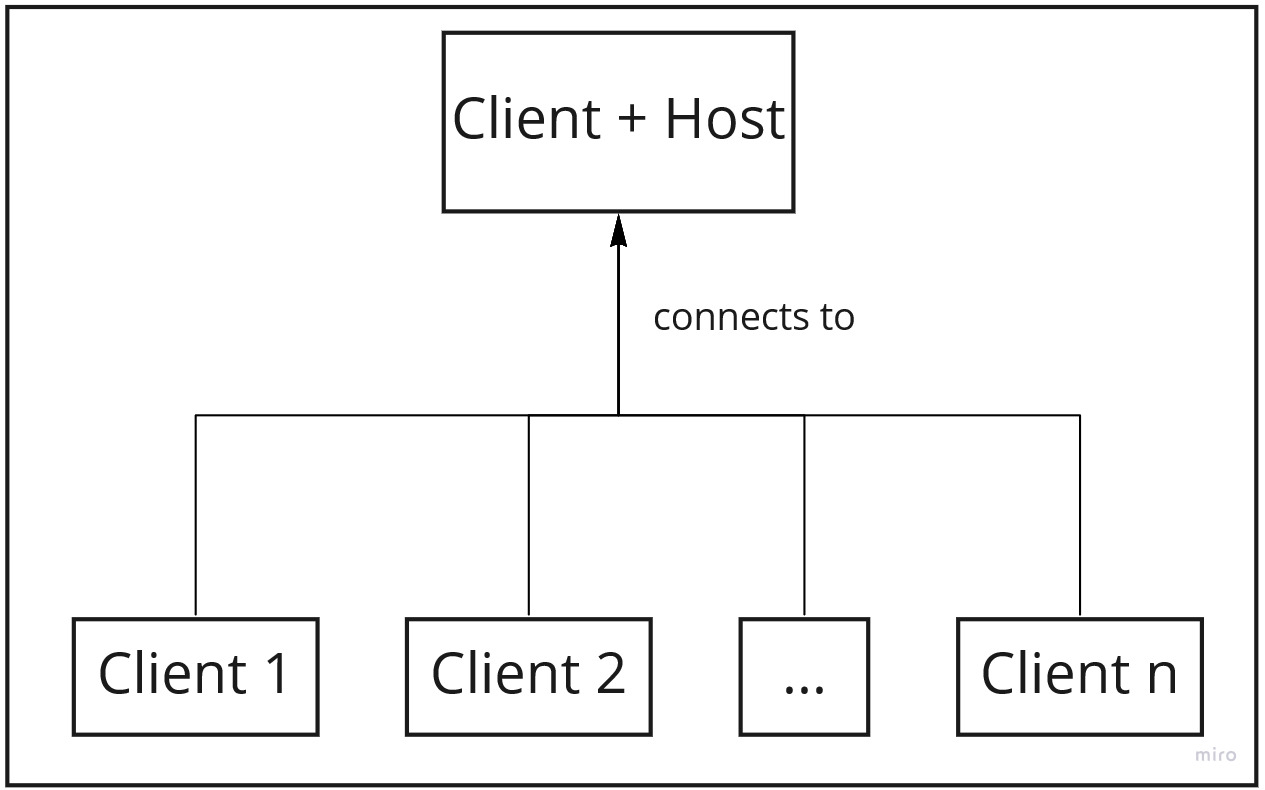
\includegraphics[width=70mm]{images/Client_Host.jpg}
	\caption[Client-Server Modell]{Das Client-Host-Modell einfach veranschaulicht}
	\label{pic:Client_Host}
\end{figure}

Bei dieser Variante wird der Serverprozess auf demselben Gerät ausgeführt, auf dem auch eine Client-Instanz gestartet wurde. Ein Spieler übernimmt also selbst das Hosting. Andere Clients haben die Information, welcher Client einen Serverprozess besitzt und wie sie sich dorthin verbinden können. 

\textbf{Vorteile:}
\begin{itemize}
	\item Die Unabhängigkeit von Hardwareressourcen für Entwickler Dieses 'Problem' wird an die Spieler ausgelagert. 
\end{itemize}

\textbf{Nachteile:} 
\begin{itemize}
	\item Da der Serverprozess nun ebenfalls auf einem Gerät läuft, auf welches Spieler Zugriff haben, gibt es ebenfalls mehr Möglichkeiten des Hacking (Spielmanipulation) \cite{Wikipedia.2021h}. Die Entwickler haben keinerlei Einfluss auf die Serverprozesse, welche ein Spieler startet. \cite{Smed.2002}
\end{itemize}

\newpage
\textsf{\Large Client Server:}

\begin{figure}[H]
\centering
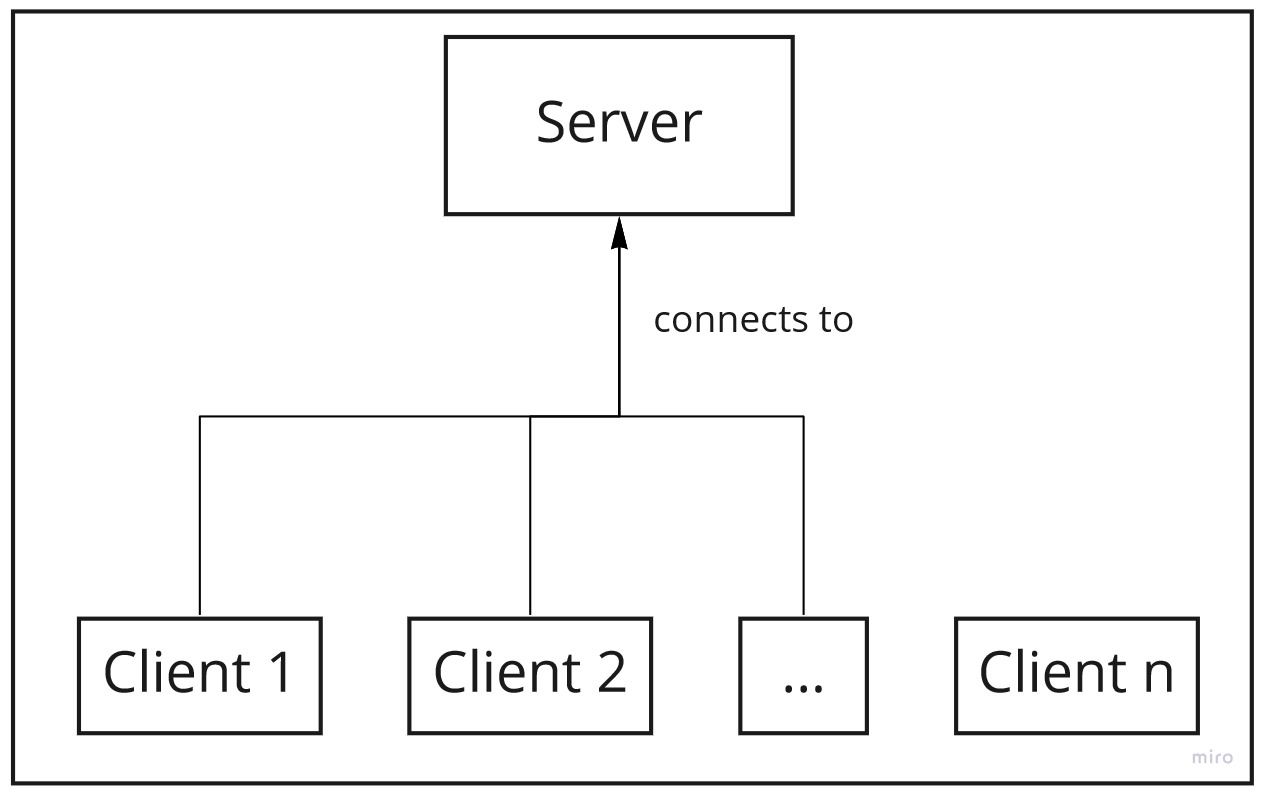
\includegraphics[width=70mm]{images/Client_Server.jpg}
\caption[Client-Server Modell]{Das Client-Server-Modell einfach veranschaulicht}
\label{pic:Client_Server}
\end{figure}

Diese Variante trennt Client und Server physikalisch voneinander. Serverprozesse werden außerhalb einer Client-Umgebung gestartet und verwaltet. Clients haben einen (oder mehrere) zentrale Zielsysteme, zu welchen sie sich verbinden können.

\textbf{Vorteile:}
\begin{itemize}
	\item Mehr Kontrolle auf Seiten der Entwickler, Hacking ist deutlich erschwert. Die Software-Architektur kann verhindern, dass spielentscheidende Daten nicht in der Hand der Spieler liegen, und somit ein sicheres und faires Spiel gewährleistet werden kann. \cite{Smed.2002}
\end{itemize}

\textbf{Nachteile:}
\begin{itemize}
	\item Die Kosten für Hardware und Bandbreite skalieren mit den Spielerzahlen. Diese Tatsache könnte sehr schnell hohe Kosten verursachen. \cite{Deng.2018}
	\item Bei einer simplen, monolithischen Architektur kann dieses Modell dazu führen, dass die Hardware, welche als Server fungiert zum 'Single Point of Failure' wird. Das bedeutet, dass ein Ausfall des zentralen Spielservers dazu führen kann, dass ein Großteil der Spielerfahrung nicht mehr spielbar ist.
\end{itemize}

\section{Datenspeicherung und Transfer}

Um das bestmögliche Spielerlebnis zu ermöglichen, sollte innerhalb der Entwicklung von Multiplayer-Spielen darauf geachtet werden, dass spielentscheidende Daten schnellstmöglich zwischen den Clients synchronisiert werden. Wie auch bei anderen Echtzeitsystemen \cite{Wikipedia.2021} kommt es also auch bei der Entwicklung von dieser Art von Software darauf an, Daten zu serialisieren (Konvertierung der Daten für die Übertragung über das Netzwerk) \cite{Wikipedia.2019}. Daten unterscheiden sich im Kontext der Online Spielentwicklung grundsätzlich nicht großartig von anderer Software. Typischerweise werden Programmiersprachen wie C\# oder C++ genutzt, um Klassen und Datenstrukturen zu erstellen, welche die eigene Spiellogik abbilden \cite{Glinka.2008}.  Das folgende Klassendiagramm zeigt zwei simple Klassen. Eine Klasse, welche den Spieler abbildet sowie eine Klasse, welche alle Spieler verwaltet.

\begin{figure}[H]
	\centering
	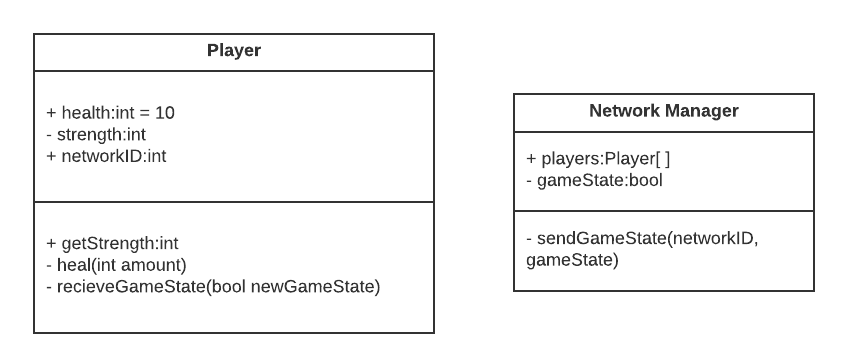
\includegraphics[width=130mm]{images/UML_class_Player_NM.png}
	\caption[UML Klassen]{UML Klasse Player und Network Manager}
	\label{pic:UML_class_Player_NM}
\end{figure}

Das Beispiel ist stark vereinfacht, soll jedoch illustrieren, auf welche Art und Weise Daten typischerweise innerhalb eines Multiplayer-Kontextes verwaltet werden. Der Entwickler entscheidet hierbei selbst, welche Informationen in welchem Kontext vorhanden ist. Konkret muss sich ein Entwickler stets die Frage stellen, ob eine Information im Server-Kontext oder im Client-Kontext verwaltet bzw. verarbeitet werden soll. Serialisierte Daten werden über ein Netzwerk transportiert. Je nach Art der Architektur erfolgt ein Umweg über eine Server-Instanz, oder direkt zu einem anderen Client. \cite{Smed.2002c}

\section{Informationskontrolle und Interest Management}

\textsf{\Large Informationskontrolle:}

'Welche Information soll zu welchem Zeitpunkt in welchem Kontext verfügbar sein?' \\
Diese Frage müssen sich Multiplayer-Spieleentwickler aus verschiedenen Gründen regelmäßig stellen. Die Gründe sind:

\textbf{Security:} \\
Beispiel: Bei einem Online-Poker Spiel wäre es fatal, wenn ein Mitspieler jederzeit über alle Karten seiner Mitspieler Kenntnis hätte. 

\textbf{Network traffic:} \\
Beispiel: In Mario Kart sammelt ein Spieler ein Item ein. Der Server würfelt für diesen Spieler ein zufälliges Item aus, welches der Spieler im Anschluss verwenden soll. Die Information über das Resultat der Zufallsauswahl sollte an den jeweiligen Spieler gesendet werden, welcher dieses Item erhalten soll. Alle anderen Spieler muss diese Information nicht interessieren.
 
\textsf{\Large Interest Management:}
\label{interest_management}

Interest Management beschreibt ein Konzept, welches delegiert, welche Informationen in welchem Kontext zu welcher Zeit für welche Personen verfügbar sind. Befindet sich der Spieler in einem bestimmten Bereich einer Spielwelt, kann das Interest Management dafür sorgen, dass dieser Spieler für manche Spieler sichtbar, und für manche Spieler nicht sichtbar ist. Die Sichtbarkeit verändert sich, je nachdem wie nahe sich die Spieler zueinander befinden, oder in welchem Areal der Spielwelt sie sich befinden.

Dieses Konzept wird besonders oft in MMO-Spielen \cite{Wikipedia.2021i} benutzt, damit ein Server mehrere Tausend Spieler ohne Abstürze verwalten kann. Ebenso wird es benutzt, um Spiellogik umzusetzen, welche es nur ausgewählten Spielern erlaubt, andere Spieler oder Objekte innerhalb der Spielwelt zu sehen und/oder mit ihnen interagieren zu dürfen. \cite{Smed.2002c}

\newpage

\section{Matchmaking}

Matchmaking bei Multiplayer Online Spielen ist ein Dienst, der es Spielern ermöglicht andere Mitspieler oder Gegner zu finden \cite{.2014}.  Die häufigsten Konzepte von Matchmaking Diensten sind:

\textbf{Playlists:} \\
Playlists sind automatisch verwaltete Ströme von Spielsitzungen, denen die Spieler nach Belieben beitreten und verlassen können. Anhand einer Reihe vordefinierter Regeln wird die Konfiguration der einzelnen Sitzungen festgelegt, ohne dass ein Mensch eingreifen muss.  

Die Spiele bieten in der Regel eine Auswahl an thematischen Wiedergabelisten (z. B. Teams oder Singleplayer, ausgefallene Regeln usw.), um verschiedenen Geschmäckern oder Stimmungen gerecht zu werden. Da die Wiedergabelisten von Servern verwaltet werden, die vom Entwickler des Spiels kontrolliert werden, können sie im Laufe der Zeit geändert werden. Wenn ein Spieler eine Wiedergabeliste auswählt, schließt er sich einem Pool von anderen Spielern an, die die gleiche Wahl getroffen haben. Der Playlist-Server verbindet sie dann entweder mit einer bestehenden Sitzung oder erstellt eine neue. 

\begin{figure}[H]
	\centering
	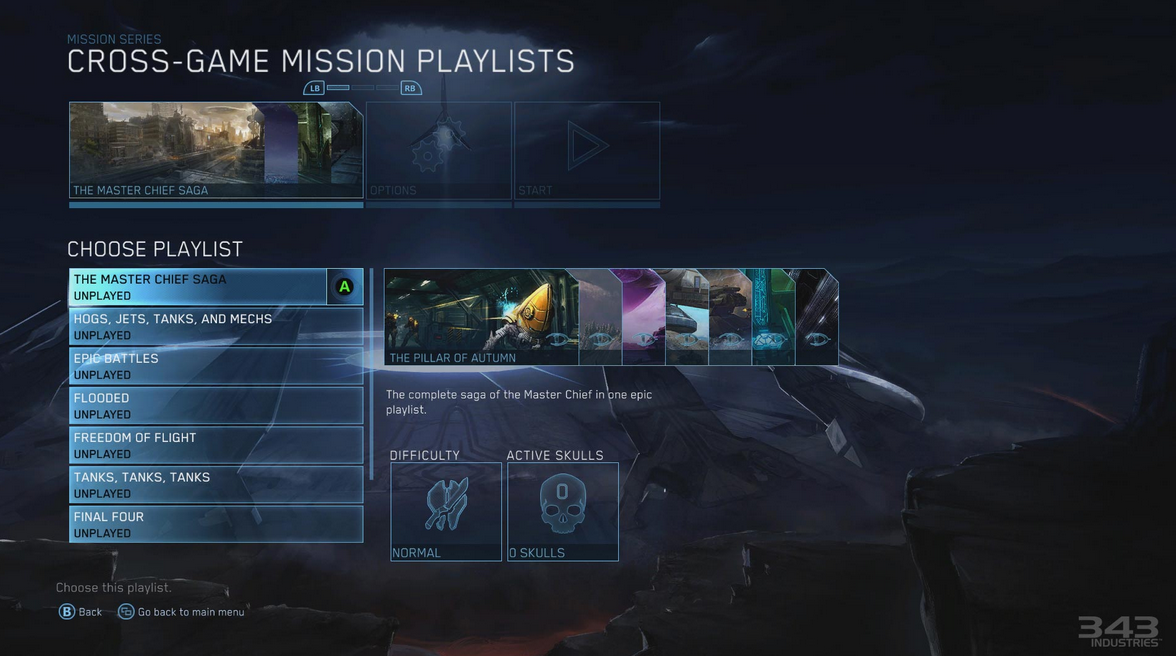
\includegraphics[width=120mm]{images/halo_playlist.png}
	\caption['Halo' Playlist]{Der Spieler muss im Spiel 'Halo' eine Playlist auswählen, um einem Spiel beizutreten.}
	\label{pic:halo_playlist}
\end{figure}

\cite{Wikipedia.2021b}

\textbf{Parties:} \\
Partys sind Gruppen von Spielern, die von Matchmaking-Systemen als eine Einheit behandelt werden. Eine Gruppe kann von Sitzung zu Sitzung wechseln, ohne dass ihre Spieler voneinander getrennt werden. Das Konzept eignet sich besonders gut für Wiedergabelisten, die automatisch die Logistik der Suche oder Erstellung von Spielsitzungen mit genügend Platz für die gesamte Gruppe übernehmen können.

\begin{figure}[H]
	\centering
	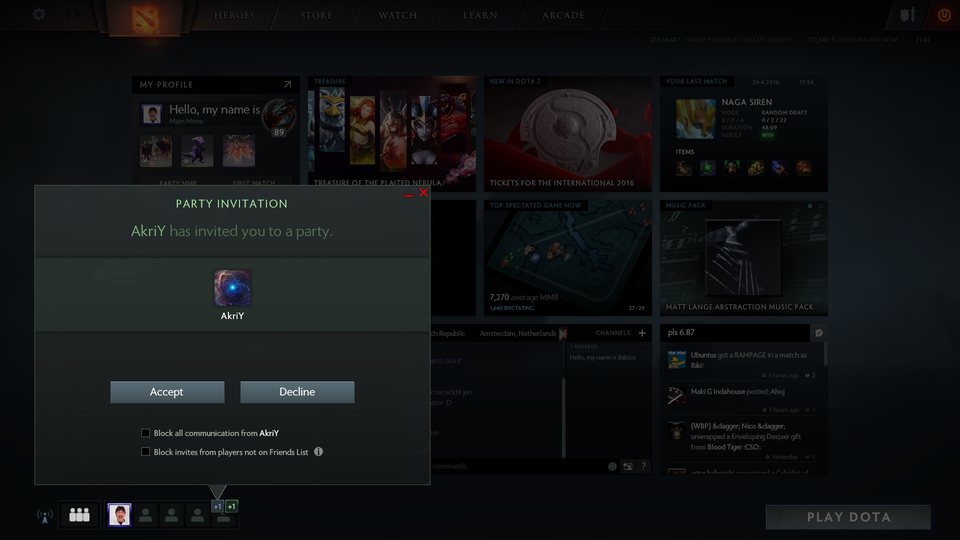
\includegraphics[width=120mm]{images/Dota2_Party_Invite.png}
	\caption['Dota 2' Party]{In 'Dota 2' wird ein Spieler von einem anderen Spieler zu einer Party eingeladen}
	\label{pic:Dota2_Party_Invite}
\end{figure}

\cite{Wikipedia.2021b} 

\textbf{Lobbys:} \\
Bei manchen Spielmodellen wird zwischen mehreren Spielszenen hin- und hergewechselt. Eine Spielszene ist eine Sammlung an Spielobjekten, Spielmenüs und Spielcharakteren, die als eine Einheit innerhalb eines Spiels zu verstehen ist. Oft sind Szenenwechsel mit Ladezeiten verbunden. Die Aufgliederung eines Spiels in Spielszenen erleichtert Entwicklern den Umgang mit limitierten Hardwareressourcen. \cite{Wikipedia.2012}

Lobbys sind Spielszenen, in denen die Spieler die bevorstehende Spielsitzung einsehen, die Ergebnisse der letzten Sitzung prüfen, ihre Einstellungen ändern und miteinander sprechen können. In vielen Spielen kehren die Spieler am Ende jeder Sitzung in die Lobby zurück. In einigen Spielen werden Spieler, die einer bereits begonnenen Sitzung beitreten, bis zum Beginn der nächsten Sitzung in der Lobby untergebracht. Da Lobbys nur wenige Ressourcen verbrauchen, werden sie manchmal zusätzlich als 'Warteschleife' für Spieler verwendet, bis ein geeigneter Gastgeber für die nächste Sitzung gefunden ist. Lobbys, die von Playlists erstellt werden, haben oft einen Countdown-Timer, bevor die Sitzung beginnt, während Lobbys, die von einem Spieler erstellt werden, im Allgemeinen nach dessen Ermessen übergehen.

\begin{figure}[H]
	\centering
	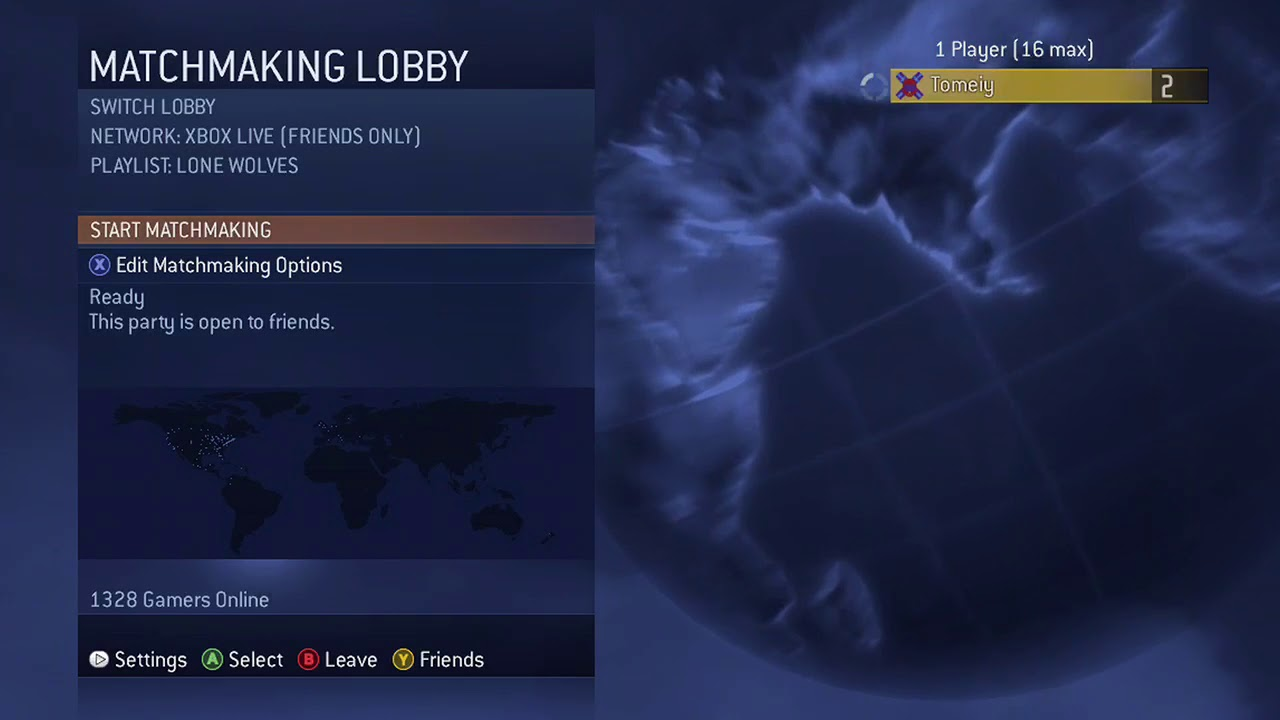
\includegraphics[width=120mm]{images/halo3_lobby.jpg}
	\caption['Halo 3' Lobby]{Eine Lobby im Spiel 'Halo 3' mit einem aktiven Spieler}
	\label{pic:Dota2_Party_Invite}
\end{figure}

\cite{Wikipedia.2021b}

\textbf{Ranking:} \\
Viele Matchmaking-Systeme verfügen über ein Ranglistensystem, mit dem versucht wird, Spieler mit ähnlichen Fähigkeiten zusammenzubringen. Spiele wie League of Legends oder die FIFA-Reihe verwenden Divisionen und Ränge für ihr Matchmaking-Bewertungssystem. Jeder Spieler tritt in verschiedenen Rängen an und für jeden Sieg gibt es Ligapunkte, für jede Niederlage werden Ligapunkte abgezogen.

Bei Spielen mit Rangliste werden in der Regel nicht gewertete Sitzungen für Spieler angeboten, die nicht wollen, dass ihre Leistung aufgezeichnet und analysiert wird. Diese werden getrennt gehalten, damit sich rangierte und nicht rangierte Spieler nicht vermischen.

\cite{Wikipedia.2021b}

\textbf{Server browsers:} \\
Einige Spiele zeigen den Spielern eine Liste aktiver Sitzungen an und ermöglichen diesen manuell eine Sitzung auszuwählen, der sie beitreten möchten. Dieses System kann in Verbindung mit Ranglisten und Lobbys verwendet werden, wird aber durch die On-Demand-Sitzungserstellung von Playlists vereitelt.

Die meisten dieser Server-Browser ermöglichen es den Spielern, die Ergebnisse zu filtern, die sie liefern. Zu den üblichen Filterkriterien gehören Servername, Spielerzahl, Spielmodus und Latenzzeit. 

\begin{figure}[H]
	\centering
	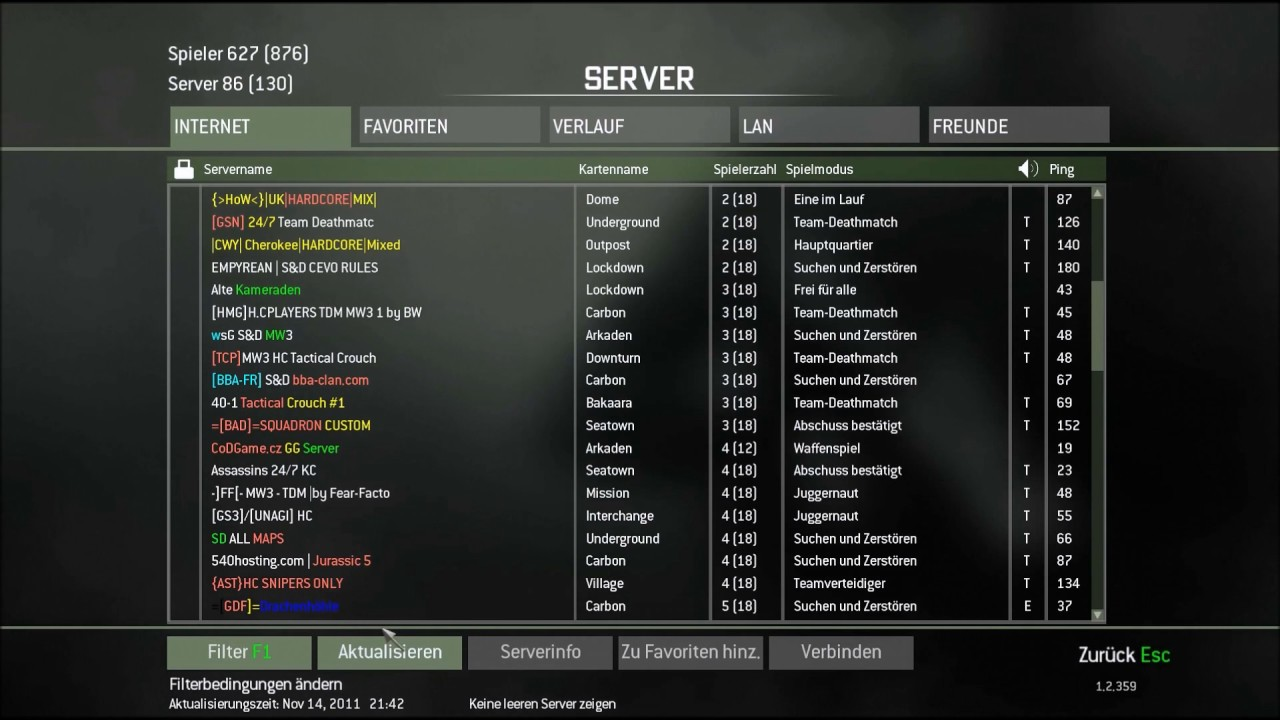
\includegraphics[width=120mm]{images/call_of_Duty_serverbrowser.jpg}
	\caption['Call of Duty Modern Warfare' Serverbrowser]{Der Serverbrowser aus dem Spiel 'Call of Duty: Modern Warfare'}
	\label{pic:call_of_Duty_serverbrowser}
\end{figure}


\cite{Wikipedia.2021b}

\textbf{Contacts lists:} \\
Eine der gängigsten Formen des Matchmaking besteht darin, den Spielern eine Liste anderer Spieler zur Verfügung zu stellen, die sie bereits kennengelernt haben und mit denen sie vielleicht wieder spielen möchten. Der Status jedes Spielers (offline, online, spielend) wird angezeigt, es besteht die Möglichkeit, einer laufenden Sitzung beizutreten.

In vielen Fällen werden die Kontaktlisten von der Plattform verwaltet, auf der ein Spiel läuft (z. B. Xbox Live, PlayStation Network, Steam), um den Spielern den Aufwand zu ersparen, viele separate Listen für viele einzelne Spiele zu verwalten. \cite{Wikipedia.2021b}

\chapter{Konzepte}
\label{sec:konzepte}

In diesem Kapitel werden abstrakte Konzepte beschrieben. Besonders unerfahrene Entwickler eines Online-Multiplayer Spiels sollen anhand dieser Konzepte Ideen für eine sinnvolle Herangehensweise erhalten, um einen roten Faden in ihrer Entwicklung verfolgen zu können. Insbesondere wenn der Entwickler noch wenig oder keine Erfahrung mit der Entwicklung von Online-Mulitplayerspielen gesammelt hat, sollen diese Konzepte bei der Erstellung einer soliden Grund-Architektur nützlich sein. Bevor eines dieser Konzepte angewandt werden kann, müssen folgende Voraussetzungen erfüllt sein:

\begin{enumerate}
	\item Das grundsätzliche Spielkonzept steht fest.
	\item Anhand des festgelegten Spielkonzeptes kann abgeschätzt werden, ob sich für das Spiel eine Client / Server oder eine Client / Host Architektur eignet.
\end{enumerate}

Sollte das Team bzw. der Solo-Entwickler zum Entschluss gekommen sein, dass sich ein Client / Server Modell am besten für den spezifischen Use Case eignet, so müssen Vorkehrungen getroffen werden, um die Hardware-Ressourcen für den späteren Server-Runner bzw. die Matchmaking API sicherzustellen. Die Grundvoraussetzung ist jedoch ein aus dem Internet erreichbarer PC mit einer festen IP-Adresse. 

Alternativ kann auch zunächst lokal innerhalb eines LAN entwickelt werden. Hierbei ist jedoch wichtig, dass eventuell auftretende Seiteneffekte, die durch Latenz oder Bandbreite verursacht werden, nicht unter Realbedingungen getestet werden können. Es empfiehlt sich deshalb bereits innerhalb der ersten Entwicklungsiterationen auszutesten, wie Prototypen für Serverprozesse auf unterschiedliche Standorte der Serverhardware reagieren. 

Nun gilt es, passende Technologien zu finden. Hier gibt es keine klare Empfehlung, jedoch können die in diesem Kapitel beschriebenen Konzepte bei der Entscheidung helfen. Es gibt bereits Frameworks \& Game Engines, die manche dieser Konzepte bereits implementiert haben und als Libraries für Entwickler bereitstellen.

\cite{MFatihMAR.2021}

\section{Vorwort zu den aufgestellten Konzepten}

Die folgenden Konzepte sollen im Kontext einer bereits erarbeiteten Spielidee eine Hilfestellung zur Erarbeitung einer individuellen technischen Architektur geben.

Konkret muss beachtet werden, dass einige der Konzepte nicht als einzelne Programm-Klassen verstanden werden müssen, sondern als Hilfestellung für Ableitungen zu konkreten Klassen oder Skripten genutzt werden können. Es ist auch gut denkbar, dass einige Implementierungen deutliche Vorteile haben, wenn bestimmte Konzepte jeweils für getrennte Spiel-Szenen umgesetzt werden. Spielszenen sind eine Beschreibung von Objekten, Lichtquellen, Materialeigenschaften sowie der Position und Blickrichtung eines virtuellen Betrachters \cite{Wikipedia.2012}.

Die Konzepte sind als separat voneinander zu betrachtende Softwarekomponenten zu sehen, die miteinander kommunizieren können. Man könnte die einzelnen implementierten Konzepte auch als Microservices \cite{Thones.2015} bezeichnen, die innerhalb eines Server-Prozesses eigene interne Abläufe besitzen und durchführen. Die Kommunikation zwischen den Komponenten sollte über direkte, gegenseitige Funktionsaufrufe oder über ereignisgesteuerte Funktionen \cite{Michelson.2006} geschehen.

\section{API für Matchmaking \& Server-Runner}

Für Spiele, welche ein Matchmaking-System benötigen, muss eine API entworfen werden, welche unabhängig von einem existierenden Client oder Serverprozess arbeitet. Diese API hat 2 grundsätzliche Aufgaben. 

\textbf{Matchmaking:}

Die API muss einen Algorithmus implementieren, welcher mehrere Spieler zu einer Spiel-Session zusammenführt. Mögliche Matchmaking-Konzepte sind bereits im Hintergrund-Kapitel beschrieben. Die Matchmaking API verwaltet als eine Liste an aktiven Serverprozessen sowie die Information, wie man sich zu ihnen verbindet. In der Regel wird pro Serverprozess ein Netzwerk-Port an der Server-Maschine reserviert, auf denen sich dann N Spieler verbinden können.

Je nach Spielkonzept können hunderte, tausende Serverprozesse existieren, welche jeweils nur eine vergleichsweise geringe Anzahl (1-20) an Spieler verwalten. Spielkonzepte, welche viele Spieler (200-1000) innerhalb eines einzigen Serverprozesses voraussetzten, erzeugen dagegen zwar quantitativ weniger Serverprozesse, diese neigen aber in der Regel schnell zu Überlastung. Neben der Umsetzung von Interest Management und einer performanten Architektur für möglichst wenig Network-Traffic, kann aber auch die Matchmaking API Abhilfe schaffen, bspw. durch 'Umverlegung' von Spielern auf andere oder neue Cluster.

\textbf{Server-Runner:}

Neben dem Matchmaking ist die API ebenfalls auch zuständig für das Starten und die Überwachung von Serverprozessen.
Ebenfalls können technische Statusinformationen über ein aktuell laufendes Spiel innerhalb eines Serverprozesses von der API verwaltet werden, beispielsweise darüber, ob es möglich ist einem Server beizutreten, oder wie viele Spieler bereits auf einem Serverprozess spielen. Die folgende Grafik visualisiert beide Aufgaben:

\begin{figure}[H]
	\centering
	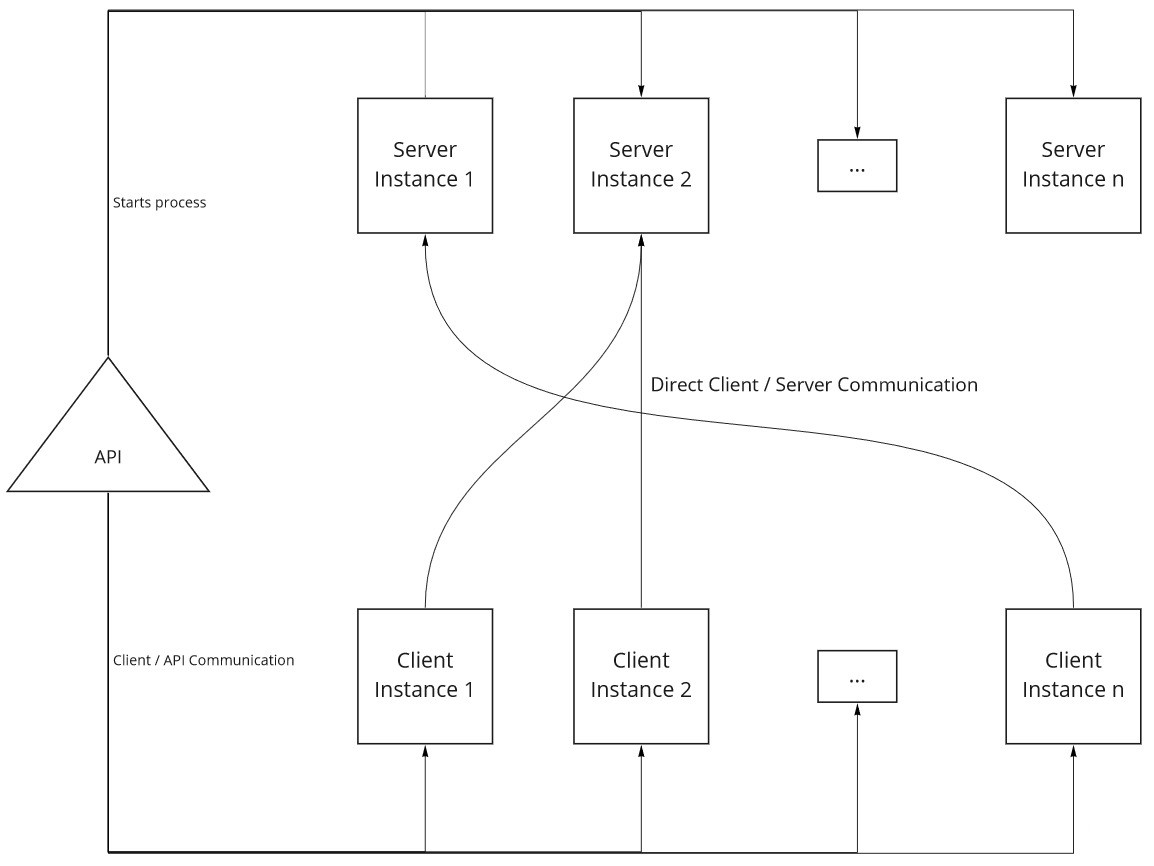
\includegraphics[width=120mm]{images/API_Konzept_Diagramm.jpg}
	\caption[API Konzept Diagramm]{Veranschaulichung des API-Konzepts}
	\label{pic:API_Konzept_Diagramm}
\end{figure}

Je nach Spiel kann das Aufgabenfeld der API um weitere Punkte erweitert werden, beispielsweise die Verwaltung einer Datenbank für Authentifizierung bzw. Kommunikation mit externen Authentifizierungs-Service-Providern, oder für einen In-Game Shop.

\section{Client UI \& Visual Controller}

Der Client UI \& Visual Controller beschreibt die Art und Weise, wie die Benutzeroberfläche und visuelle Ebene eines Spielers durch Antworten des Servers oder einzelner Spieleraktivitäten manipuliert wird.

Konkret sorgt ein Server-Ereignis, der Input eines Spielers (beispielsweise durch Klicken eines Buttons oder einsammeln eines Gegenstands) oder ein anderes Ereignis dafür, dass Funktionen innerhalb des Client UI \& Visual Controllers aufgerufen werden. Innerhalb dieser Funktionen werden Komponenten der Benutzeroberfläche wie z. B. Anzeigetexte, Bilder etc. oder Objekte innerhalb der Spielwelt selbst manipuliert. In der folgenden Grafik zeigt die beschriebene Folge an Ereignissen:

\begin{figure}[H]
	\centering
	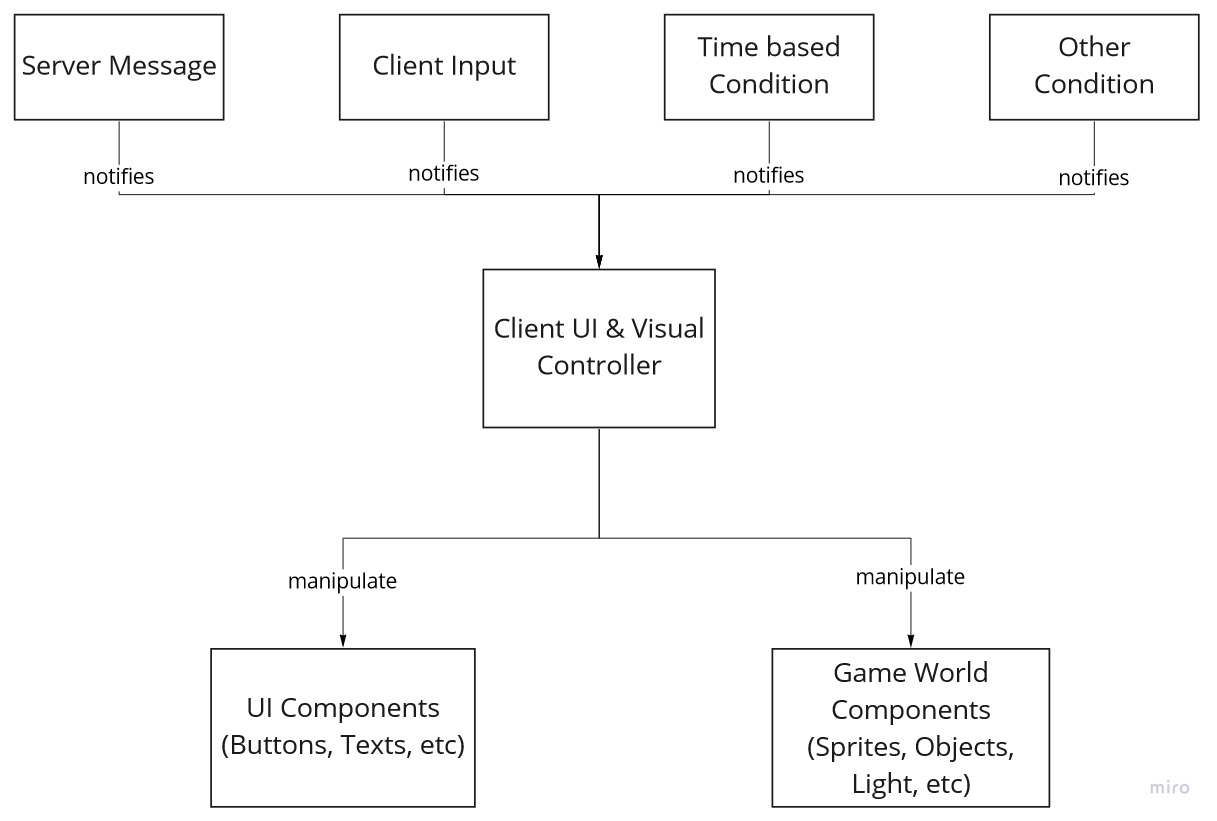
\includegraphics[width=100mm]{images/Client_UI_und_Visual_Konzept.jpg}
	\caption[Client UI \& Visual Controller Diagramm]{Veranschaulichung des Client UI \& Visual Controller Konzepts}
	\label{pic:Client_UI_und_Visual_Konzept}
\end{figure}

Wichtig ist, dass Funktionen des Client UI \& Visual Controller erst nach server- oder clientseitigen Überprüfungen ausgeführt werden. Der Controller selbst sollte nur überprüfen, ob fluktuierende Komponenten noch existieren, oder sich in einem konsistenten Zustand befinden. Spiel-Relevante Logik, beispielsweise, ob ein Spieler berechtigt ist, bestimmte Aktionen durchzuführen, ist nicht Teil des Client UI \& Visual Controllers.

\section{Server Network Manager}

Der Server Network Manager ist für die korrekte Abarbeitung von serverseitigen Aufgaben zuständig, welche aufkommen, sobald ein Netzwerk-spezifisches Ereignis stattfindet.

\textbf{Beispiel:} \\
Die Verbindung eines Clients bricht mitten in der laufenden Spielszene ab. Der Server Network Manager stößt infolgedessen Funktionen anderer serverseitigen Manager-Komponenten an, welche dafür sorgen, dass alle Spieler über den neuen Zustand des Spiels informiert werden. Hierfür müssen zunächst serverinterne Variablen aktualisiert werden.

\textbf{Beispiel:}  \\
In einem Online-Ableger des Spiels 'Mensch ärgere dich nicht' verliert ein Spieler seine Netzwerkverbindung. Als Reaktion kümmert sich der Server Network Manager darum, dass das Spiel trotzdem zu Ende gespielt werden kann. Die Spielfiguren des ausgeschiedenen Spielers müssen entfernt, und der Spiel-Fortschritt aktualisiert werden. Diese Funktionen stellt möglicherweise der \hyperref[spawn_manager]{Runtime Spawn Manager}, \hyperref[progress_manager]{Progress / Game State Manager } zur Verfügung.
Außerdem muss dem \hyperref[serverside_client_manager]{Serverside Client Manager} mitgeteilt werden, dass dieser Spieler nun nicht mehr Teil der Spiel-Session ist.

Die folgende Grafik illustriert die Aufgaben des Server Network Managers:

\begin{figure}[H]
	\centering
	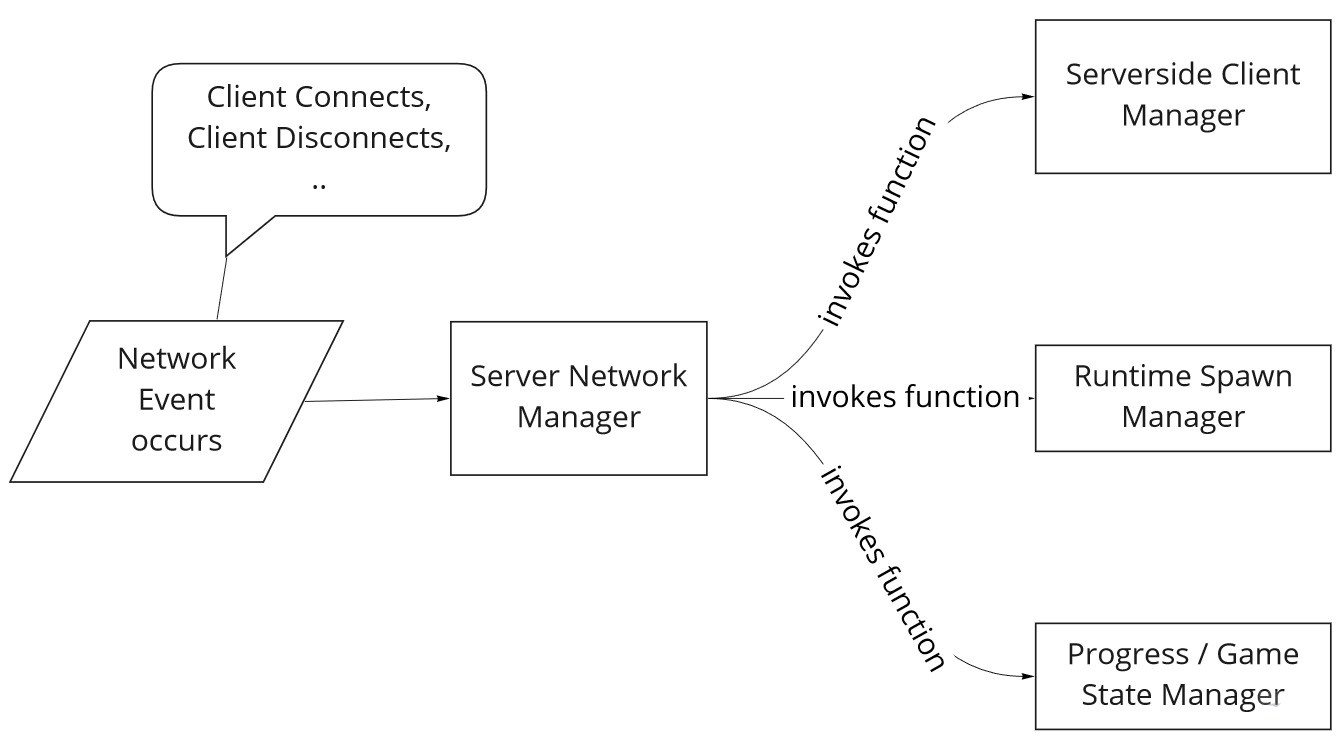
\includegraphics[width=110mm]{images/Server_Network_Manager.jpg}
	\caption[Server Network Manager Diagramm]{Veranschaulichung des Server Network Manager Konzepts}
	\label{pic:Server_Network_Manager}
\end{figure}

\section{Lobby / Multi Scene Manager}

Der Lobby/ Multi Scene Manager ist eine serverseitige Komponente, welche es erlaubt, Spielszenen-übergreifende Informationen zu speichern und zu verwalten. Beispielsweise könnte bei einem Lobby-basierten Matchmaking die Information des Leiters einer Lobby über Spielszenen hinweg gespeichert werden. Ebenso wäre es denkbar, dass der Bereitschafts-Status vor dem tatsächlichen Spiel innerhalb des Lobby / Multi Scene Managers gespeichert wird. Außerdem stellt der Lobby / Multi Scene Manager Funktionen bereit, welche

\begin{itemize}
	\item alle Clients informiert, sobald ein globaler Szenenwechsel angestoßen werden soll
	\item alle Clients über den aktuellen Status einer Lobby informiert.
\end{itemize}

\begin{figure}[H]
	\centering
	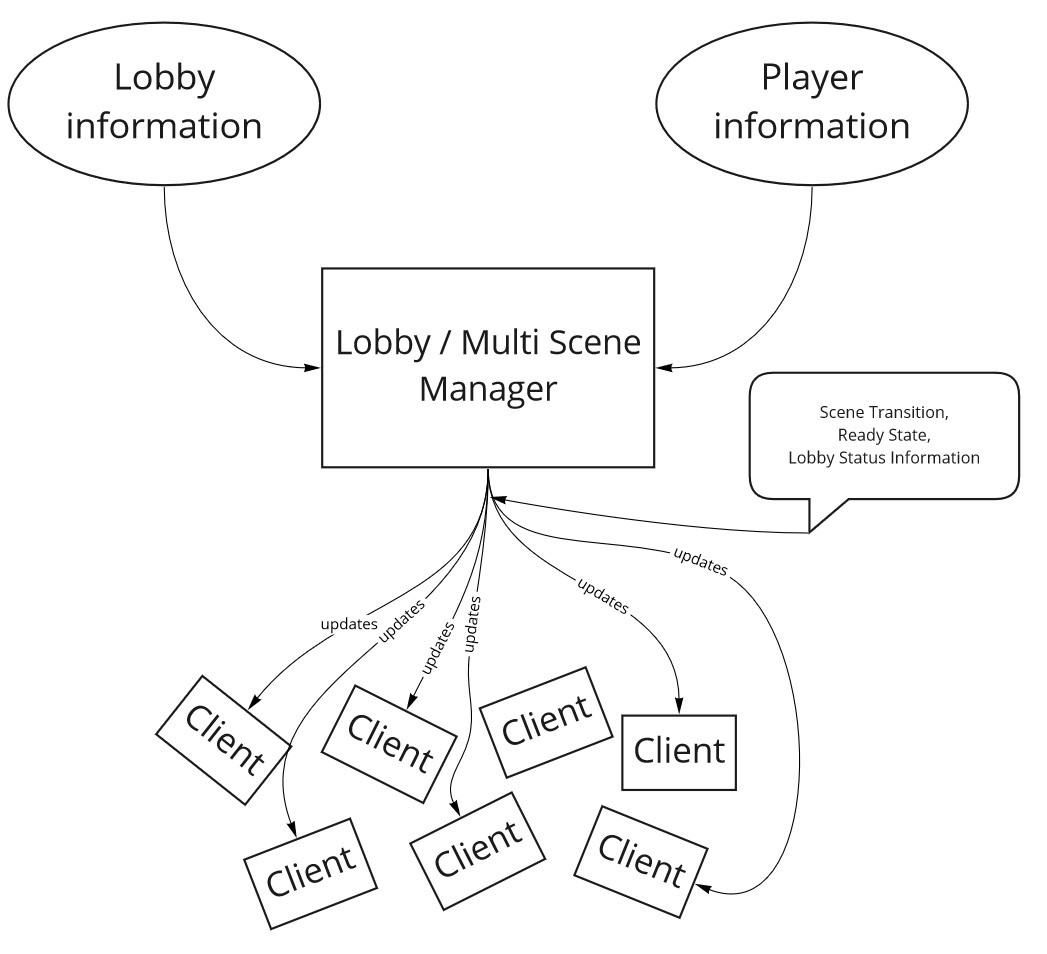
\includegraphics[width=110mm]{images/Lobby_Multi_Scene_Manager.jpg}
	\caption[Lobby / Mutli Scene Manager Diagramm]{Veranschaulichung des Lobby / Mutli Scene Manager Konzepts}
	\label{pic:Lobby_Multi_Scene_Manager}
\end{figure}


\section{Client Connection Manager}

Der Client Connection Manager beschreibt eine Softwarekomponente, welche folgende Aufgaben umsetzen muss:

 \begin{itemize}
	\item Implementierung von clientseitigen Methoden zum Informationsaustausch mit Matchmaking API.
	\begin{itemize}
		\item Z. B. stellt die Matchmaking API dem Client über HTTP-Kommunikation Informationen bereit, mit denen sich der Client auf einen speziellen Server verbinden kann (IP + Port). \cite{Wikipedia.2021d} \cite{Wikipedia.2021e}
	\end{itemize}
	\item Verarbeitung der von Matchmaking API bereitgestellten Informationen. 
	\begin{itemize}
		\item Z. B. könnte die Matchmaking API einem Client die Information bereitstellen, dass aus einem bestimmten Grund dem angeforderten Serverbeitritt verweigert wird. Diese Information muss der Client Connection Manager zwischenspeichern und verwalten.
	\end{itemize}
	\item Aufruf von Methoden eines Client UI Controllers.
	\begin{itemize}
		\item Z. B. Die soeben erlangte Information über den verweigerten Serverbeitritt muss nun dem Nutzer dargestellt werden, hierfür ruft der Client Connection Manager Funktionen auf, welche ein Client UI Controller implementiert hat.
	\end{itemize}
	\item Ausführen von Handler-Funktionen und Auslösen von Events für clientseitige Konsequenzen bei Netzwerkabbruch, manuellem Verlassen einer Server-Session oder sonstigen Abbruchgründen, welche dazu führen, dass eine Online-Spielsession verlassen wird.
	\begin{itemize}
		\item Z. B. wird die notwendige Verbindung zum Internet während des Spiels unterbrochen. Der Client Connection Manager löst Callbacks aus, welche im Client UI \& Visual Controller implementiert sind. Diese sorgen dafür, dass der Spieler zurück ins Hauptmenü geleitet wird, in dem eine Fehlermeldung dargestellt wird, welche erklärt, warum das Spiel abgebrochen ist.
	\end{itemize}
	\item Bereitstellung von Funktionen, welche den Beitritt zu einem Game-Server sicherstellen.
\end{itemize}


\begin{figure}[H]
	\centering
	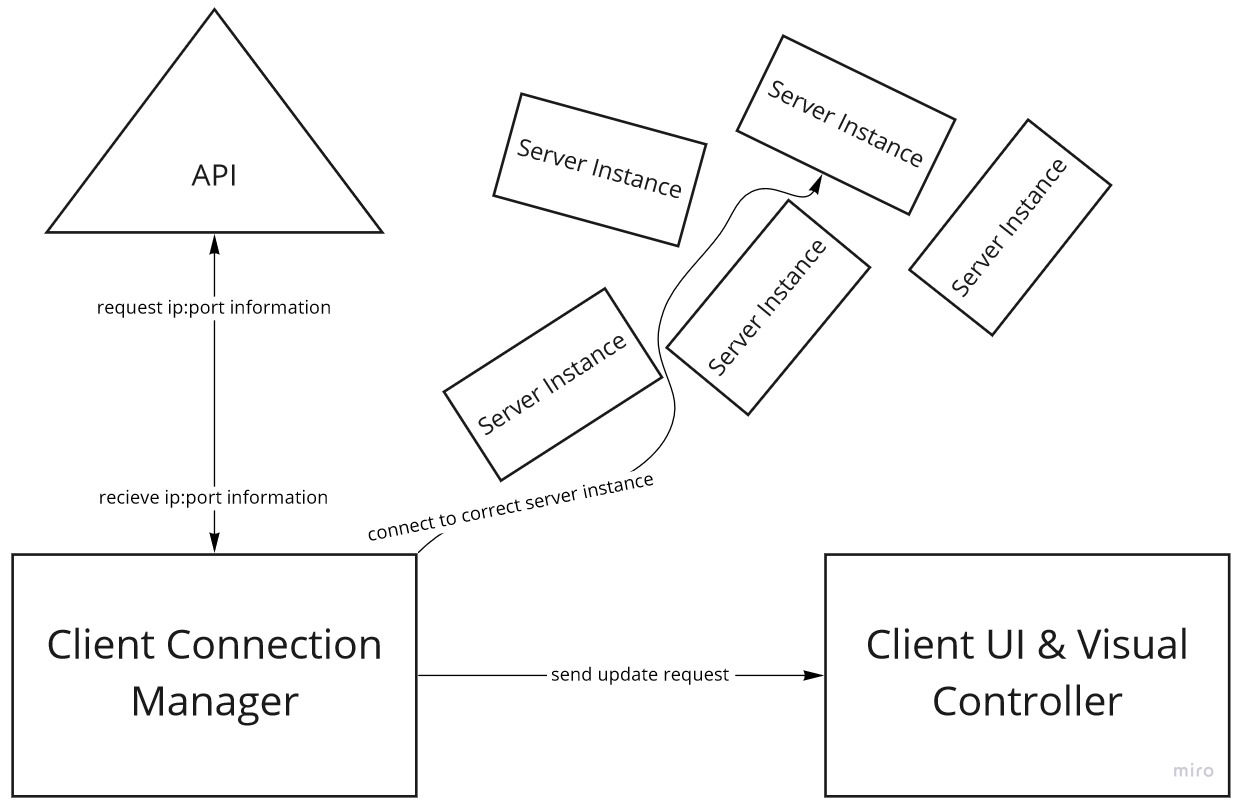
\includegraphics[width=100mm]{images/Client_Connection_Manager.jpg}
	\caption[Client Connection Manager Diagramm]{Veranschaulichung des Client Connection Manager Konzepts}
	\label{pic:Client_Connection_Manager}
\end{figure}

\section{Serverside Client Manager}

\label{serverside_client_manager}

Das Konzept des serverseitigen Client Managers beinhaltet die Verwaltung aller verbundener Clients innerhalb eines aktiven Serverprozesses. Insbesondere speichert der serverseitige Client Manager 2 Arten von Information über jeden Client:

Einerseits werden netzwerkbezogene Informationen über einen Client gespeichert, im einfachsten Fall ist dies lediglich die IP-Adresse des Hosts sowie der Port, auf welchem der Server seinen Kommunikationskanal geöffnet hat. Bei Spielkonzepten, welche eine weitergehende Authentifizierung des Spielers voraussetzen, können hier auch Benutzernamen, Benutzertags, E-Mail-Adressen o. ä. gespeichert und weiterverarbeitet werden. Zum Anderen speichert und verwaltet der serverseitige Client Manager auch spielespezifische Informationen wie bspw. den aktuellen Anzeigenamen, konfigurierte Individualisierung des Spielcharakters, Spielerrollen oder andere Eigenschaften, über die der Server während einer Spiel-Session Kenntnis haben sollte. Die folgende Grafik visualisiert diesen Informationsfluss:

\begin{figure}[H]
	\centering
	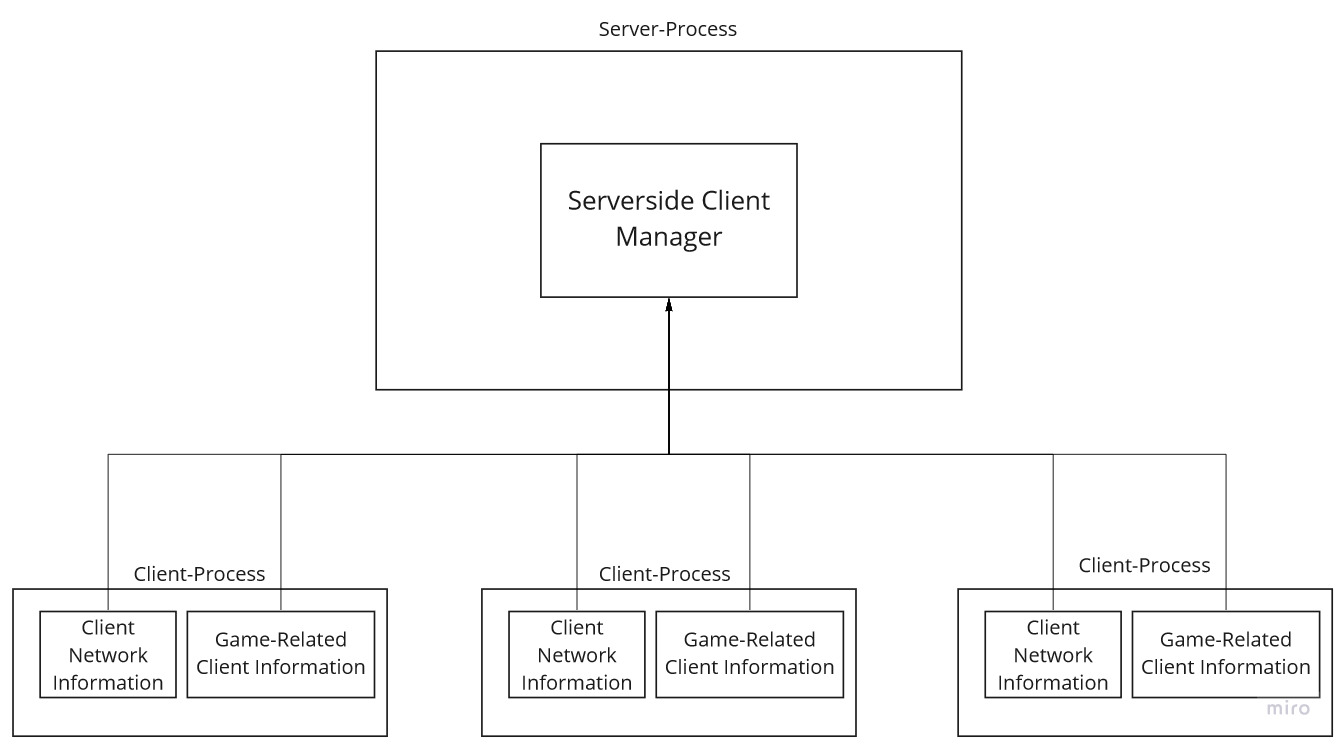
\includegraphics[width=120mm]{images/serversided_client_manager.jpg}
	\caption[Serversided Client Manager]{Veranschaulichung des serverseitigen Client Manager Konzepts}
	\label{pic:serversided_client_manager}
\end{figure}

\section{Prepare-Game-Manager}

Der Prepare-Game-Manager ist Teil des Serverprozesses und beinhaltet alle Funktionen, welche nötig sind, um eine Spielszene aufzubauen, bevor die Spieler ihr beitreten dürfen. Die Funktionen sollten konkret umsetzen:

\begin{itemize}
	\item Spawning \cite{Wikipedia.2020} von NPCs \cite{Wikipedia.2021f} oder Spielgegenständen, die in Abhängigkeit zur Anzahl der beitretenden Spieler, einer Spielkonfiguration oder sonstigen Parametern stehen.
	\item Anpassung der Eigenschaften von bereits gespawnten NPCs oder Spielgegenständen, die in Abhängigkeit zur Anzahl der beitretenden Spieler, einer Spielkonfiguration oder sonstigen Parametern stehen.
	\item Initialisierung der Spawnpunkte für Spieler anhand von Spawnalgorithmen oder festgelegten Punkten in der Spielwelt.
	\item Abarbeitung sonstiger serverseitigen Abläufe, welche Voraussetzung für den Start des Spiels sind.
\end{itemize}

Das folgende Diagramm zeigt, wann der Prepare-Game-Manager bei einem lobby-basierten Spielkonzept zum Einsatz kommt:

\begin{figure}[H]
	\centering
	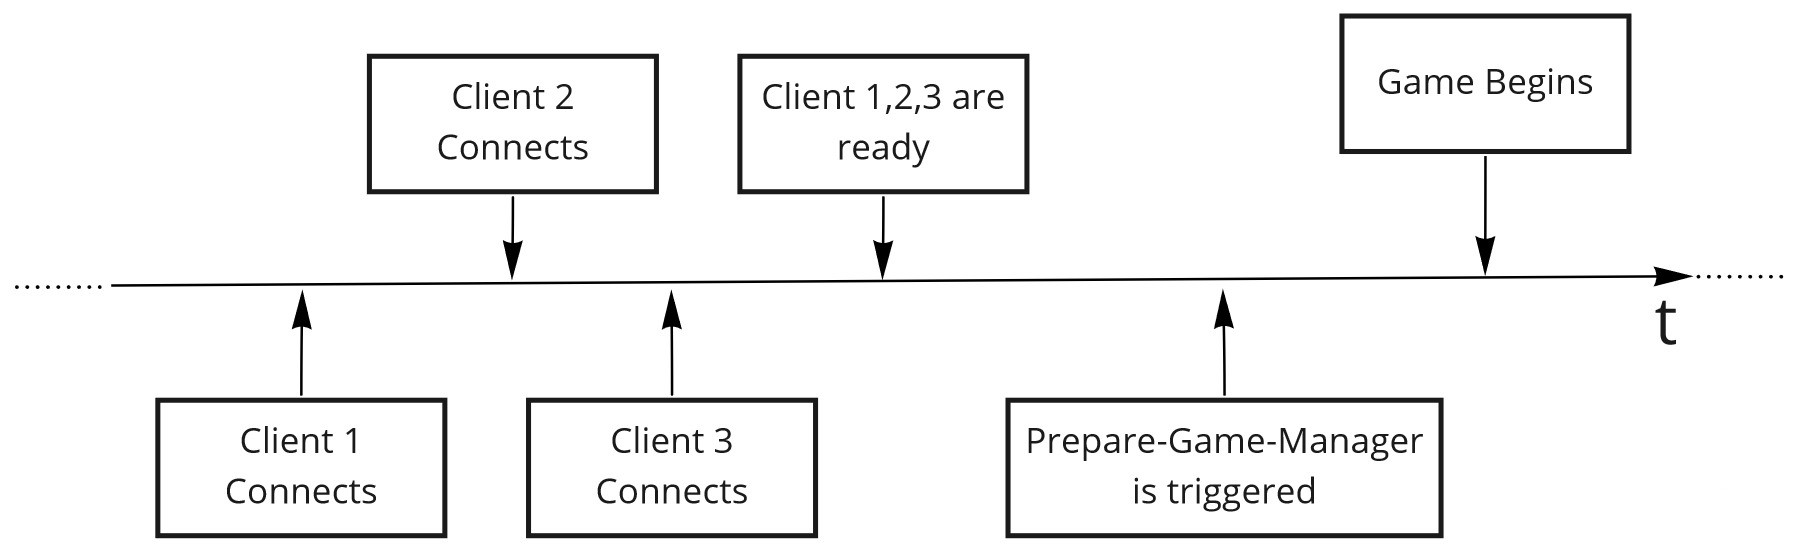
\includegraphics[width=100mm]{images/prepare_game_manager.jpg}
	\caption[Prepare-Game-Manager]{Veranschaulichung des Prepare Game Manager Konzepts}
	\label{pic:prepare_game_manager}
\end{figure}

\section{Progress / Game-State Manager}
\label{progress_manager}

Die Aufgabe eines Progress bzw. Game-State Managers ist es, Gewinn- bzw. Verlustbedingungen einer Spielsession zu speichern und zu verwalten. 

Beispiele hierfür sind: \\
\begin{itemize}
	\item Verwaltung und Synchronisierung von globalen Timern.
	\item Verwaltung und Synchronisierung von Spiel-Kennzahlen bzw. Variablen (z. B. der Spielstand bei einem Fußball-Match).
\end{itemize}

Außerdem ist der Progress Manager / Game-State Manager dafür verantwortlich, alle Clients über spielentscheidende Ereignisse zu informieren. Die Abfolge dieser Ereignisse werden im folgenden Diagramm aufgezeigt:

\begin{figure}[H]
	\centering
	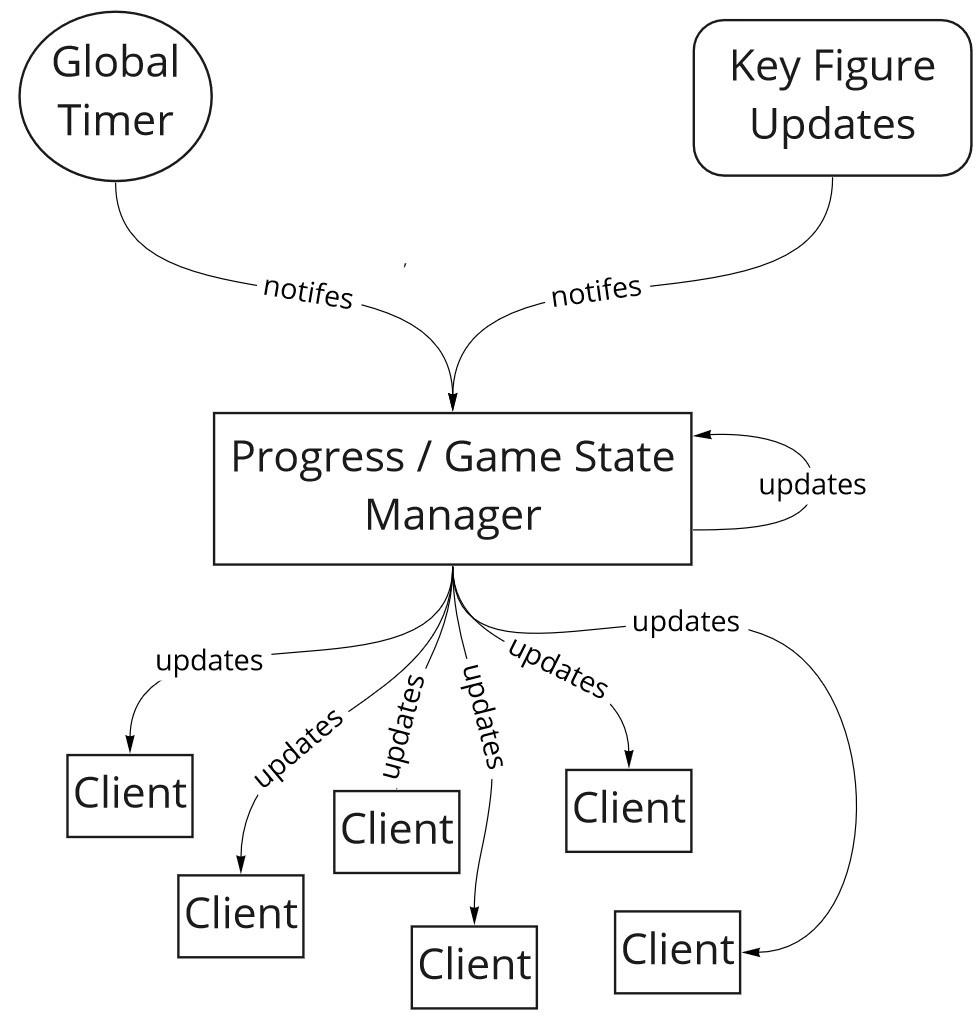
\includegraphics[width=75mm]{images/Progress_State_Manager.jpg}
	\caption[Progress / Game-State Manager]{Veranschaulichung des Progress / Game-State Manager Konzepts}
	\label{pic:Progress_State_Manager}
\end{figure}

\section{Runtime Spawn Manager}
\label{spawn_manager}

Der Runtime Spawn Manager verwaltet die zur Laufzeit zu erzeugenden Spieler- und Nicht-Spieler-Objekte. Konkret werden Funktionen des Runtime Spawn Managers ausgeführt, wenn ein spezifisches Event innerhalb einer Spiel-Session ausgelöst wird oder ein Spieler- bzw. Nicht-Spieler-Charakter stirbt und diese erneut an anderer Position spawnen sollen ('Re-Spawning'). Die Logik, wo genau ein Spieler oder Nicht-Spieler Objekt seine neue Einstiegsposition erhält, regelt ebenfalls der Runtime Spawn-Manager.

\begin{figure}[H]
	\centering
	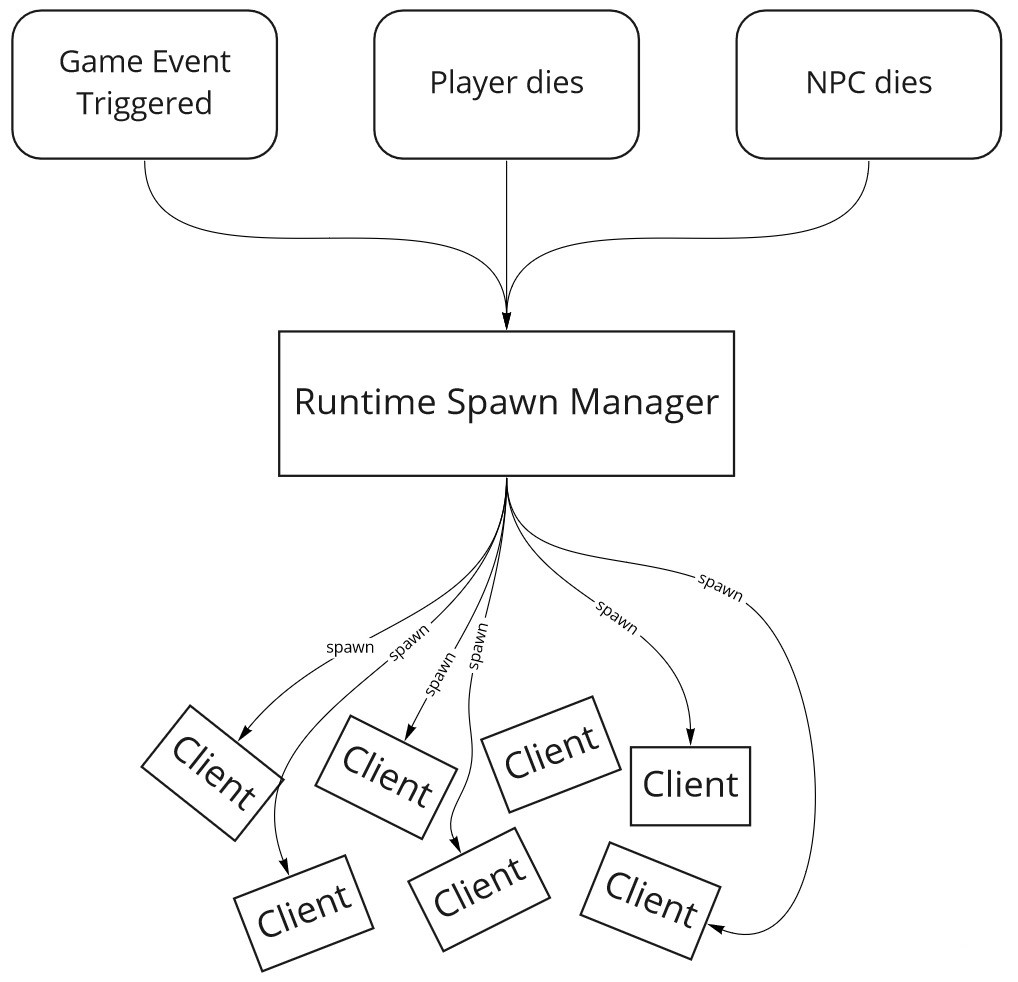
\includegraphics[width=75mm]{images/Runtime_Spawn_Manager.jpg}
	\caption[Runtime Spawn Manager]{Veranschaulichung des Runtime Spawn Manager Konzepts}
	\label{pic:Runtime_Spawn_Manager}
\end{figure}

\textbf{Beispiel:} \\
In einem Online Multiplayer Ego-Shooter \cite{Wikipedia.2021g} stirbt ein Spieler durch Schüsse anderer Spieler. Der Runtime Spawn Manager sorgt dafür, dass anhand von bestimmten, zur Laufzeit ausgerechneten Bedingungen eine neue Spawn-Position für den gestorbenen Spieler gefunden wird. 


\section{Interest Manager}

Der Interest Manager kümmert sich um die Sichtbarkeit von Objekten. Wie bereits in der Sektion über \hyperref[interest_management]{Interest Management} erklärt, ist es je nach Spielkonzept notwendig, dass der Spieler stets nur über den für ihn relevanten Teil der Spielwelt Kenntnis hat. Aus diesem Grund sollten sich angehende Spieler-Entwickler fragen, ob sie eine solche Software-Komponente in die Architektur ihres Projekts integrieren möchten. Die folgende Grafik veranschaulicht diese Aufgabe:

\begin{figure}[H]
	\centering
	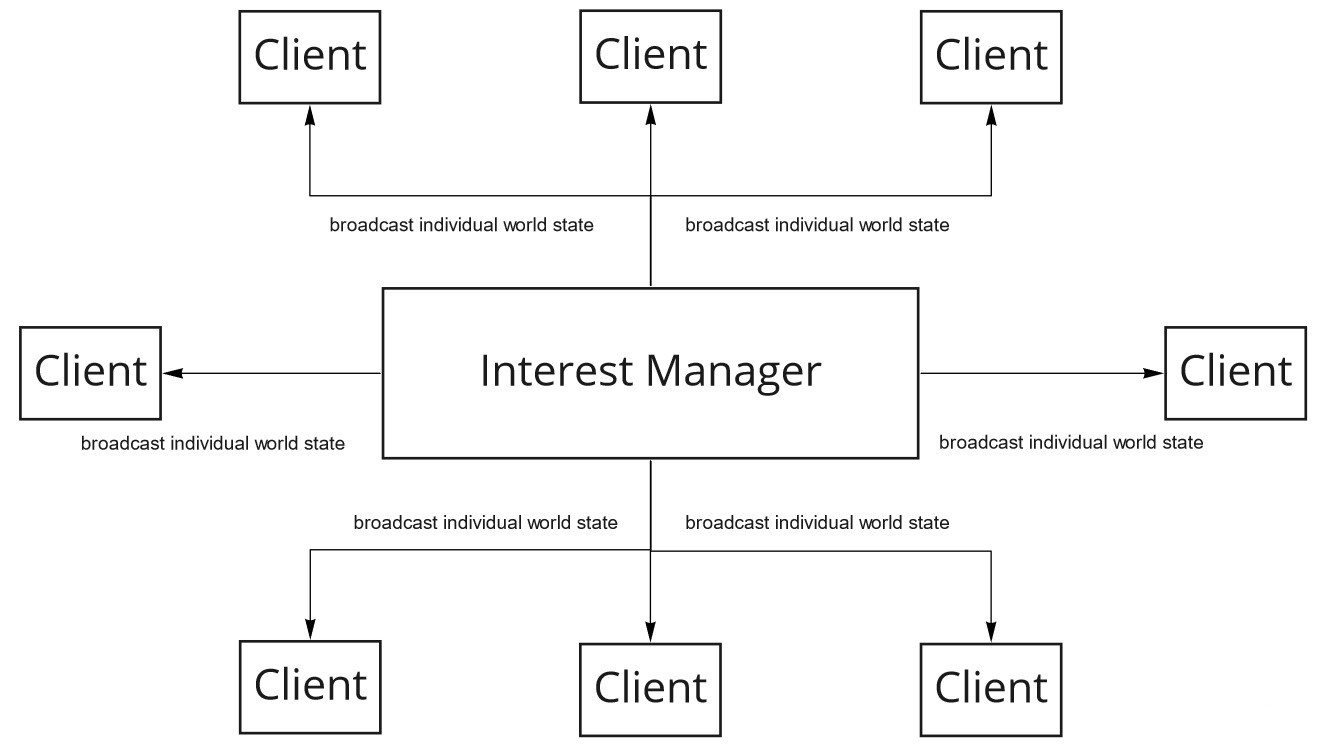
\includegraphics[width=100mm]{images/Interest_Manager.jpg}
	\caption[Interest Manager]{Veranschaulichung des Interest Manager Konzepts}
	\label{pic:Interest_Manager}
\end{figure}

Mögliche Faktoren, die der Interest Manager benutzen kann, um den Spielern die Objekte anzeigen zu lassen, die sie sehen dürfen sind:

\begin{itemize}
	\item Distanz zwischen Spieler und anderen Objekten
	\item Teams bzw. Gruppen. Die registrierten (Spieler)-Objekte innerhalb eines Teams/ einer Gruppe sind für Spieler, welche ebenfalls innerhalb des Teams/Gruppe registriert sind, sichtbar.
	\item Spatial Hashing / Grid Checker: Die Spielwelt und ihre Objekte werden in quadratische Zellen eingeteilt. Je nachdem in welcher Zelle sich ein Spieler befindet, werden nur diejenigen Objekte der Spielwelt mit dem Spieler synchronisiert, welche sich innerhalb der 8 'Nachbarzellen' befinden: 
	\begin{figure}[H]
		\centering
		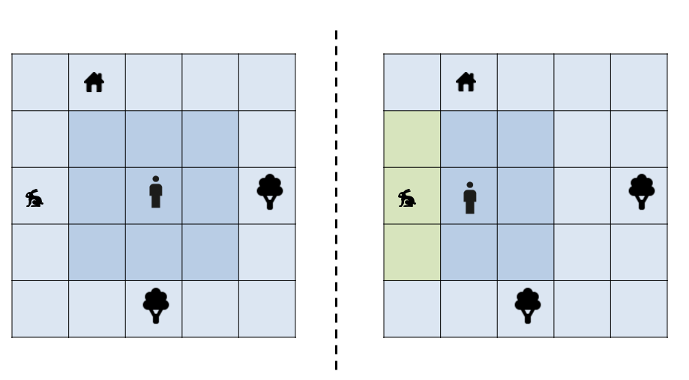
\includegraphics[width=70mm]{images/interest_management.png}
		\caption[Spatial Hashing]{Illustration des Interest Management Konzepts Spatial Hashing. \cite{JeromeRenaux.2017} }
		\label{pic:interest_management}
	\end{figure}
\end{itemize}

Sollte keine der hier beschriebenen Beispiele auf das gewünschte Spielkonzept passen, so ist es notwendig, eine eigene Logik für das Interest Management zu implementieren.

\chapter{Realisierung}
\label{sec:realisierung}

In diesem Kapitel werden die im vorherigen Kapitel beschriebenen Konzepte anhand von einem Prototypen implementiert. Die konkrete Logik wird bei jedem implementierten Konzept anhand von Code erläutert.

\section{Eingesetzte Technologien}

Für die Entwicklung des Prototyps kamen folgende Technologien zum Einsatz:

Als Game-Engine wurde Unity \cite{Technologies.03.02.2022} benutzt. Die Entscheidung hierfür begründet sich durch die gute Dokumentation und den Long-Time-Support der verschiedenen Unity Versionen. Außerdem gibt es eine große Anzahl an Benutzer. Unity existiert bereits seit dem Jahr 2005 \cite{Wikipedia.2022c}, und hat sich seitdem in Entwickler-Kreisen einen nachhaltigen Ruf erarbeitet.

C\# kommt als Programmiersprache zum Einsatz. Unity hat eine sehr gute Unterstützung hierfür.

Zusätzlich zu Unity wurde Mirror\cite{.03.02.2022} als weiteres Framework benutzt. Mirror ist eine kostenloses Open Source Networking Bibliothek, welche die Entwicklung von Netzwerk-Code deutlich erleichtert.

\section{Spielidee des Prototyps}
\label{Spielidee}

Das Grundprinzip des Prototyps basiert auf dem Kinderspiel 'Fangen und Verstecken'. Hinzu kommen weitere Spiel-Elemente, die in dieser Sektion erläutert werden. Innerhalb der Spielwelt existieren 2 verschiedene Teams, welche ausschließlich aus Spielern bestehen.

Spieler mit der Rolle 'Hider' und 'Ghost' gehören zu einem Team.  Spieler mit der Rolle 'Seeker' bilden das zweite Team. Anfangs wird per Zufall entschieden, welche Spieler zum Team 'Hider/Ghost' und welche zum Team 'Seeker' gehören. Alle Teammitglieder des Teams 'Hider/Ghost' beginnen das Spiel initial als 'Hider'. Der Leiter einer Lobby kann festlegen, ob ein oder zwei Seeker ausgewürfelt werden sollen. Zum Leiter einer Lobby wird derjenige Spieler, der als erstes einer Lobby beitritt. Sollte der Leiter einer Lobby diese verlassen, so wird der Spieler zum Leiter, der am längsten Mitglied der selben Lobby war.

Die Aufgaben der Spieler sind je nach Rolle unterschiedlich:

\textbf{Hider:}
Spieler mit der Rolle Hider haben die Aufgabe, bestimmte Objekte in der Spielwelt zu finden, und diese zu einem Zielort zu bringen. Sind alle Objekte zu ihrem Zielort gebracht, so hat das Team 'Hider/Ghost' das Spiel gewonnen. Hider müssen außerdem vor den Spielern mit der Rolle 'Seeker' flüchten, bzw. sich vor diesen verstecken. 

\textbf{Seeker:}
Spieler mit der Rolle Seeker haben lediglich eine Aufgabe. Sie müssen alle Spieler mit der Rolle 'Hider' fangen. Dies können sie tun, indem sie in die unmittelbare Reichweite eines Hiders laufen, und die Taste 'E' bzw. den in der Benutzeroberfäche festgelegten Knopf 'Catch' drücken. Sind alle Hider gefangen, so gewinnen die Seeker das Spiel.

\textbf{Ghost:}
Spieler, welche initial mit der Rolle 'Hider' gespawnt sind, und von einem Seeker gefangen wurden, wechseln ihre Rolle zu 'Ghost'. Ghosts dürfen nicht mehr mit Objekten der Spielwelt interagieren, sie können sich lediglich noch über das Spielfeld bewegen. Außerdem bekommt ein Ghost eine Fähigkeit, welche er einsetzen kann, um seinem Team zu helfen. Diese Fähigkeit bemächtet den Spieler einen Seeker für 3 Sekunden bewegungsunfähig zu machen, sollte der Spieler in der unmittelbaren Nähe eines Seekers sein, und die Taste 'E' bzw. den dafür vorgesehen Knopf in der Benutzeroberfläche drücken. Diese Fähigkeit kann lediglich alle 30 Sekunden eingesetzt werden.

\begin{figure}
	\centering
	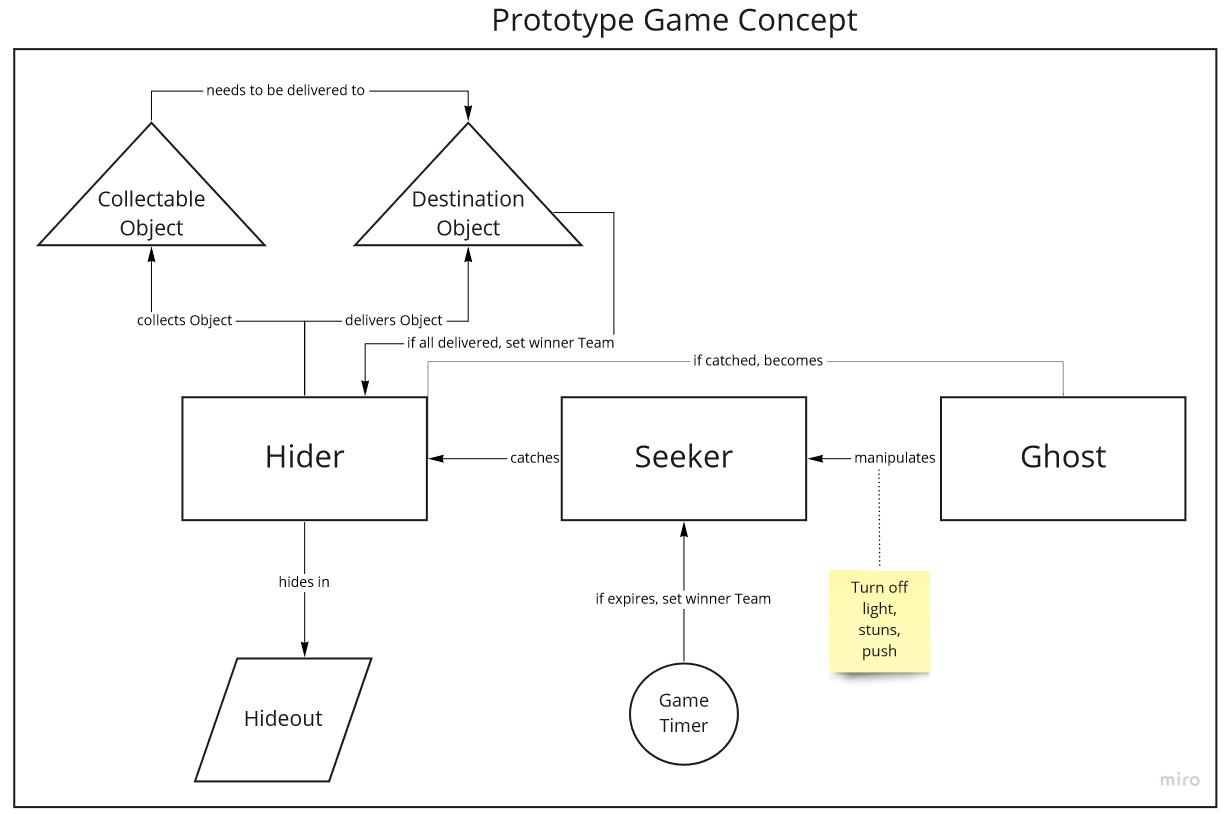
\includegraphics[width=150mm]{images/game_concept.jpg}
	\caption[Spielkonzept Diagramm]{Veranschaulichung des Spielkonzepts}
	\label{pic:game_concept}
\end{figure}

\textbf{Spiel-Ablauf:}

Zunächst muss ein Spieler eine Lobby erstellen. Dies tut er, indem er auf den Knopf 'Create Lobby' im Hauptmenü drückt. Nun erhält dieser Spieler einen 'Code', welcher eindeutig diese Lobby identifiziert. Diesen Code kann der Spieler nun an seine Mitspieler weitergeben. Diese können den Code im Hauptmenü in ein Eingabefeld eingeben, und auf 'Join Lobby' drücken. Der Spieler, welcher die Lobby erstellt hat, ist nun auch Lobby-Leiter und kann einstellen, ob die Lobby als 'public' markiert werden soll. In diesem Fall können andere Spieler durch den Button 'Join Random Lobby' ebenfalls der Lobby beitreten, ohne den Code zu kennen. 

\begin{figure}
	\centering
	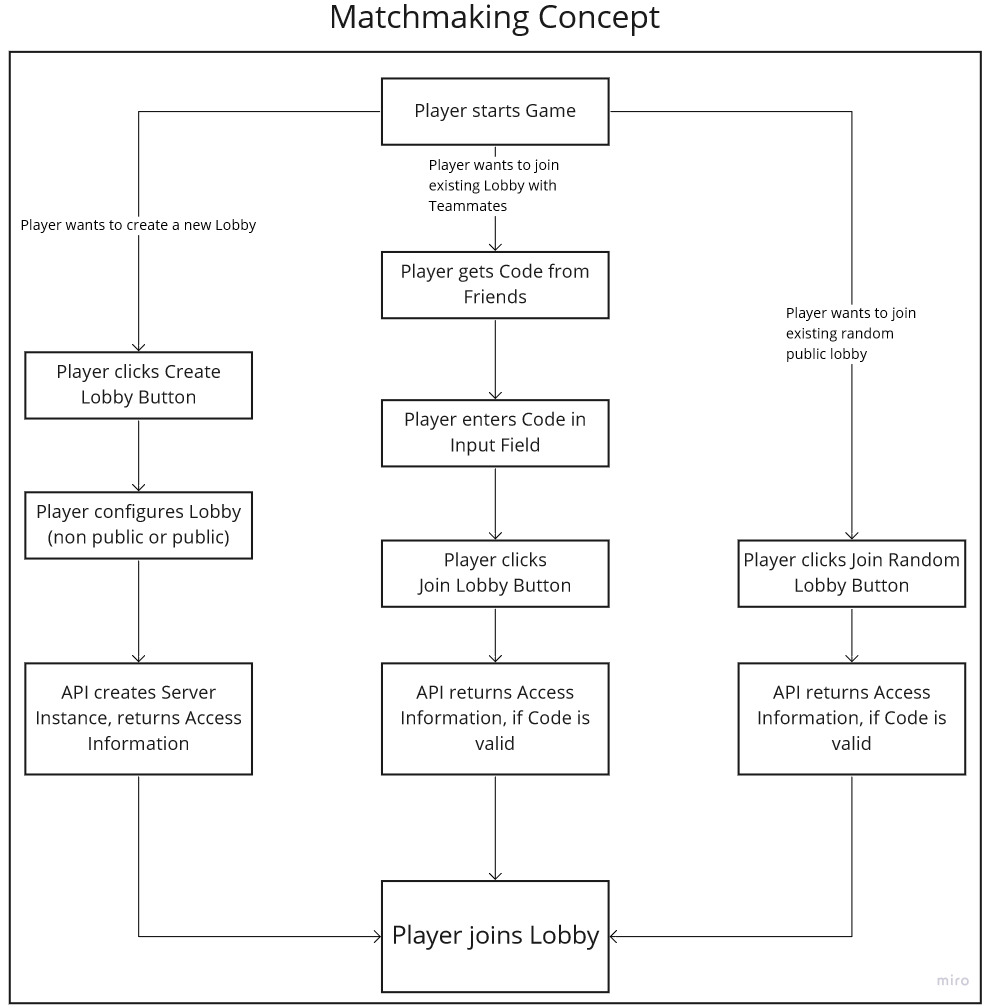
\includegraphics[width=150mm]{images/matchmaking_concept.jpg}
	\caption[Matchmaking-Konzept Diagramm]{Veranschaulichung des Matchmaking Konzepts}
	\label{pic:matchmaking_concept}
\end{figure}

Ist nun eine Lobby erstellt, und es sind mindestens 2 und maximal 10 Spieler der Lobby beigetreten, welche ihren Bereitschaftsstatus durch das drücken des Knopfes 'Ready' kommuniziert haben, so hat der Lobby-Leiter die Möglichkeit durch Drücken des Buttons 'Start Game' das Spiel zu starten.

Aus insgesamt 10 möglichen Spawn-Punkten würfelt der Prepare-Game-Manager Spawn-Punkte für die beigetretenen Spieler aus. Sobald alle Spieler die Spiel-Szene geladen haben, und auf ihrem Startpunken stehen beginnt das Spiel. Ab diesem Zeitpunkt läuft eine Stoppuhr ab, erreicht diese den Wert '0' bevor alle Objekte an ihren Zielart gebracht wurden, so hat das Team 'Seeker' gewonnen.

\section{Architektur des Prototyps}
\label{Architektur}

\textbf{Matchmaking:}
Die Matchmaking Architektur basiert auf einem Client Server Modell, sowie dem Einsatz einer REST API, welche als Matchmaking- und Server-Runner Schnittstelle dient. Der oben beschriebene Ablauf zum Beitreten einer Lobby ist im folgenden Diagramm noch einmal aus technischer Sicht visualisiert:

\begin{figure}
	\centering
	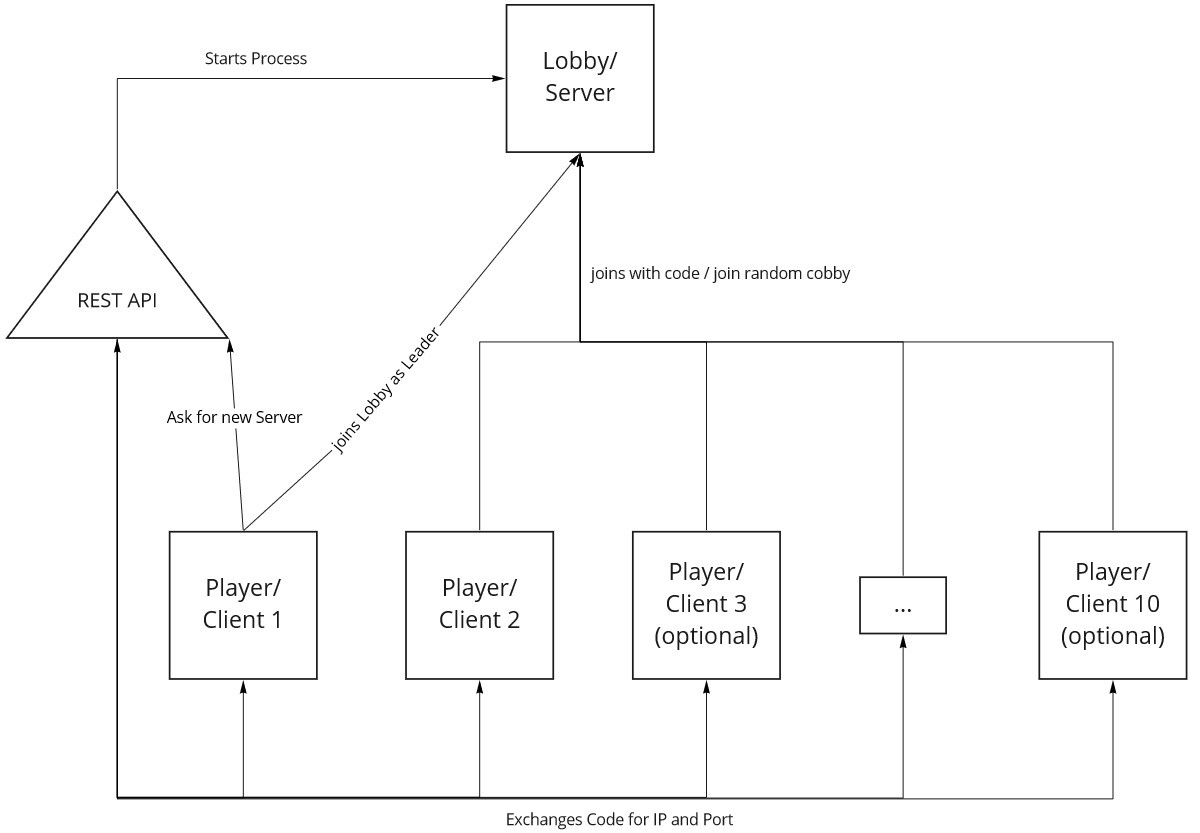
\includegraphics[width=150mm]{images/prototype_architecture_matchmaking.jpg}
	\caption[Architektur Matchmaking Diagramm]{Veranschaulichung der Architektur des Matchmakings im Prototyp}
	\label{pic:prototype_architecture_matchmaking}
\end{figure}

\textbf{Szenen:}

Im Prototypen gibt es lediglich 2 Szenen: Die Menü-Szene (Menu Scene) und die Spielszene (Game Scene).
Die Menu Scene gliedert sich in 2 verschiedene Sub-Menüs. Das 'Main Menu' wird zu Spielstart angezeigt, sowie wenn ein Spieler die Verbindung zu einem Server abbricht oder verliert. Das 'Lobby Menu' wird angezeigt, sobald ein Spieler einer Lobby beigetreten ist. 

Die Game Scene wird geladen sobald ein Spiel aus dem 'Lobby Menu' heraus gestartet wird. Das ist dann der Fall, sobald alle Mitglieder einer Lobby auf den Button 'Ready' gedrückt haben, und der Leiter dieser Lobby auf den Button 'Start Game' gedrückt hat. 

\begin{figure}
	\centering
	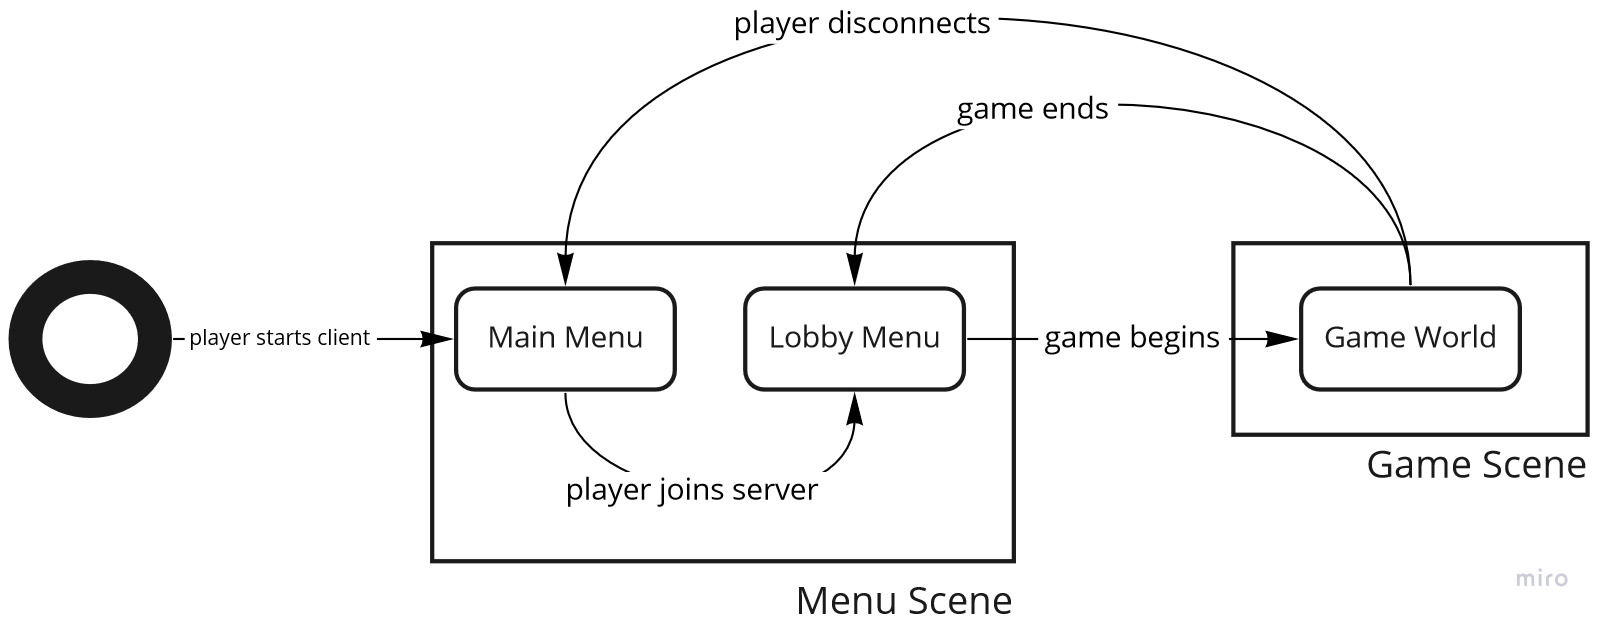
\includegraphics[width=150mm]{images/scene_architecture.jpg}
	\caption[Architektur Szenen Diagramm]{Veranschaulichung der Szenen-Architektur im Prototyp}
	\label{pic:prototype_architecture_matchmaking}
\end{figure}

Auf die Implementierungen der einzelnen Konzepte wird in den kommenden Sektionen im Detail eingegangen. Die folgende Grafik zeigt die Relationen zwischen den implementierten Konzepten untereinander:

\begin{figure}
	\centering
	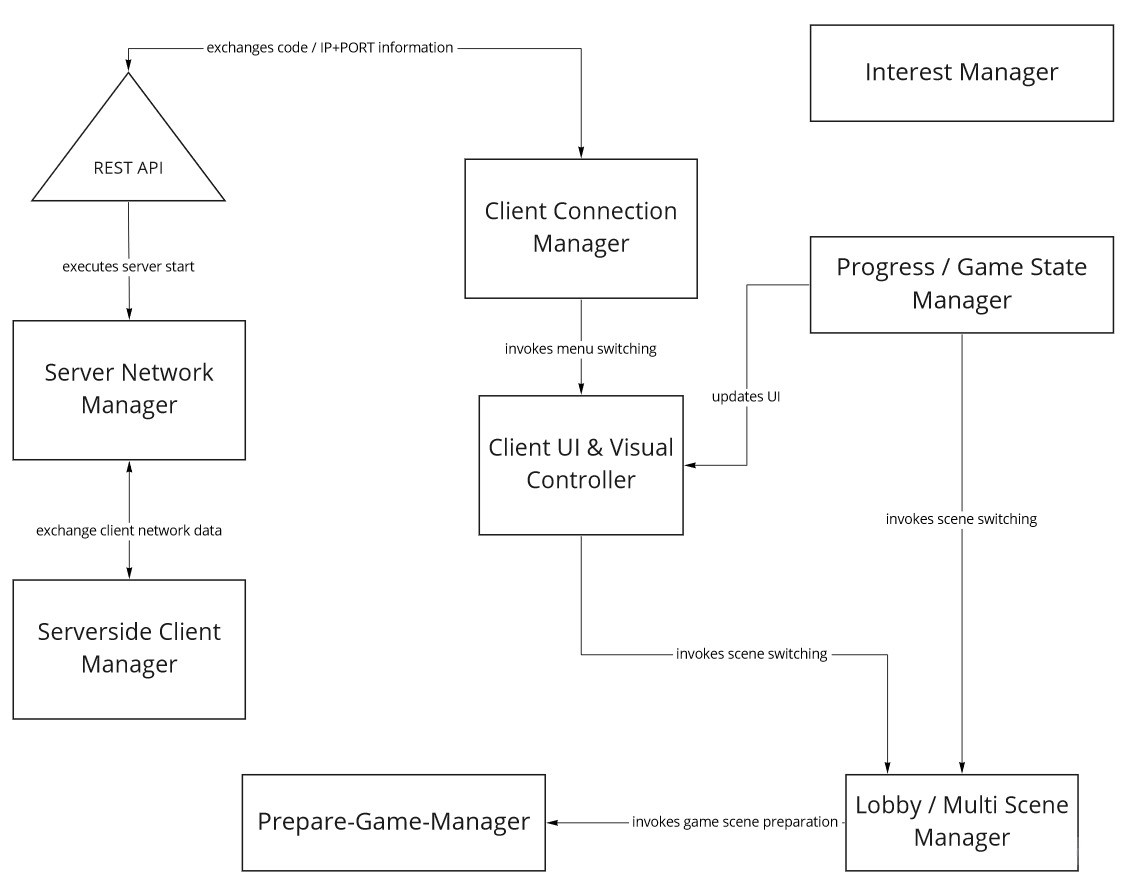
\includegraphics[width=150mm]{images/concept_relations.jpg}
	\caption[Architektur Konzept Relationen]{Veranschaulichung der Konzept Relationen im Prototyp}
	\label{pic:concept_relations}
\end{figure}

\section{Implementierung: API für Matchmaking \& Server Runner}

// TODO: Add Content

\section{Implementierung: Client UI \& Visual Controller}
\label{implementierung:client_UI_Controller}

Der Client UI \& Visual Controller spielt im Prototyp eine wesentliche Rolle. Er kommt in der GameScene als Singleton \cite{M.Gatrell.2009} zum Einsatz, wo er alle nötigen Methoden implementiert, um das lokale UI des Spielers manipulieren zu können. Hier sind nun 3 Beispiele aufgeführt:

Die folgenden 'Update' Methode ist eine Unity bereitgestellte Schnittstelle. Der Rumpf der Update Methode ist nie vorgegeben, und muss vom Entwickler selbst implementiert werden. Unity führt diese Methode jedes 'Frame' (Einzelbild) \cite{Wikipedia.2021j} aus. Dies ermöglicht eine nahezu vollständige Echtzeitabfrage der Inputs (Tastatur / Maus / andere Eingangsgeräte) des Spielers.

Im unten wird dauerhaft abgefragt, ob ein Spieler die Taste 'E' oder 'Q' auf seiner Tastatur drückt. Wenn er das tut, und ebenfalls ein paar andere Randbedingungen erfüllt sind, so wird ein 'Linksklick' auf den im UI des Spielers sichtbaren Button simuliert.

\begin{lstlisting}[caption= InGameUiControllerScript.cs Update Method]
private void Update()
{
	if (Input.GetKeyDown(KeyCode.E) && hotkeyImage != null && hotkeyImage.sprite == HOTKEY_KEYBOARD_E && interactButton.GetComponent<Button>().interactable )
	{
		interactButton.GetComponent<Button>().onClick.Invoke();
	}
	if (Input.GetKeyDown(KeyCode.Q) && lightButton.GetComponent<Button>().interactable)
	{
		lightButton.GetComponent<Button>().onClick.Invoke();
	}
}
\end{lstlisting}

Doch was heißt das genau? Im folgenden Code wird ein Event definiert, welches durch andere Klassen 'aboniert' werden kann. Wird dann das Event durch .Invoke() ausgelöst, so werden alle Funktionen in externen Skripten ausgeführt, die dieses Event aboniert haben. Hier zunächst die Definition des Events im InGameUiControllerScript und die Funktion 'clickInteractButton', die ausgeführt wird, wenn beispiese wie im obrigen Code die Taste 'E' auf der Tastatur gedrückt wird.

\begin{lstlisting}[caption= InGameUiControllerScript.cs OnInteractButtonClick Event]
public event Action OnInteractButtonClick;	

public void clickInteractButton()
{
	OnInteractButtonClick?.Invoke();
}
\end{lstlisting}

Um den gesamten Aufrufstapel\cite{Wikipedia.2021k} nachvollziehen zu können, folgt nun ein Beispiel aus einem anderen Script.
Die Klasse 'HiderScript.cs' aboniert nun in seiner Methode 'RpcEnableHideButton()' das Event des InGameUiControllerScript Singletons 'OnInteractButtonClick' mit seiner eigenen Methode 'OnHiderHideButtonClick()'. Die Methode 'RpcEnableHideButton()' wird dann ausgeführt, wenn der Server einem Spieler mit der Roller 'Hider' erlaubt, ein Versteck betreten zu dürfen.

\begin{lstlisting}[caption= HiderScript.cs Subscribe to InGameUiControllerScript Event]
[TargetRpc]
private void RpcEnableHideButton()
{
	InGameUiControllerScript.singleton.resetInteractButtonClickEvents();
	InGameUiControllerScript.singleton.OnInteractButtonClick += OnHiderHideButtonClick;
	InGameUiControllerScript.singleton.setInteractButtonEnabled(true);
	InGameUiControllerScript.singleton.setInteractButtonTextAndHotkeyImage('Hide');
}
\end{lstlisting}

Sollte der Hider nun auf seinen 'Interact'-Button drücken, so wird die folgende Methode 'OnHiderHideButtonClick()' aufgerufen. Diese ruft eine weitere Methode 'CmdHideHider()' auf, welche einen Remote Procedure Call\cite{.05.02.2022} zum Server darstellt.

\begin{lstlisting}[caption= HiderScript.csOnHiderHideButtonClick() Method]

[Client]
private void OnHiderHideButtonClick()
{
	if (enabled)
	{
		CmdHideHider();
	}
}

\end{lstlisting}

Der Server führt nun innerhalb des Methodenrumpfs von 'CmdHideHider()' einige Überprüfungen durch, ändert server-interne Variablen und sorgt somit dafür, dass alle Spieler darüber bescheid wissen, dass sich der Spieler nun in einem Versteck befindet.

\begin{lstlisting}[caption= HiderScript.cs Subscribe to InGameUiControllerScript Event]
	
	[Command]
	private void CmdHideHider()
	{
		if(vicinityScript.getHideoutObjectScript() != null)
		{
			HideableObjectScript curHideoutScript = vicinityScript.getHideoutObjectScript();
			if (!vicinityScript.getHideoutObjectScript().getIsTaken())
			{
				GetComponent<PlayerBaseScript>().setCurHideout(curHideoutScript.gameObject);
				curHideoutScript.setIsTaken(true);
				curHideoutScript.setCurrentHider(gameObject);
				isHiding = true;
				GetComponent<PlayerBaseScript>().playerLightEnabled = false;
				GameNetworkManager.FindObject(gameObject, 'FeetTrigger').SetActive(!isHiding);
				RpcNotifyHideState(true, GameNetworkManager.singleton.getConfiguredPlayerSpeed());
				RpcEnableLeaveHideoutButton();
				GetComponent<PlayerBaseScript>().TargetEnableLightButton(false);
			}
			else
			{
				RpcDisableInteractButton();
			}
		}
	}	
\end{lstlisting}

Die nächste Beispielmethode implementiert die Logik, den Interact-Button selbst aktiv- und inaktiv zu setzen. Der Interact Button selbst verfügt ebenfalls über ein 'HotkeyImage', welches einem visuellen Indikator gleich kommt, der die aktuell zu drückende Taste auf der Tastatur darstellt. Dieser Indikator wird bei jedem Aufruf von setInteractButtonEnabled ebenfalls an - oder ausgeschaltet.

\begin{lstlisting}[caption= InGameUiControllerScript.cs setInteractButtonEnabled]
public void setInteractButtonEnabled(bool enabled)
	{
		interactButton.GetComponent<Button>().interactable = enabled;
		if(hotkeyImage != null)
		hotkeyImage.gameObject.SetActive(enabled);
	}
\end{lstlisting}

Das letzte Beispiel ist eine Implementung eines simplen Flip-Mechanismus bei Betätigen des Light-Buttons (An- und ausschalten der Taschenlampe eines Spielers). Diese Logik tauscht lediglich das Bild (Sprite) aus, welches auf dem Button liegt.

\begin{lstlisting}[caption= InGameUiControllerScript.cs flipLightButtonImage]
public void flipLightButtonImage()
{
	if (!lightOn)
	{
		lightButton.GetComponent<Image>().sprite = lightOnSprite;
	}
	else
	{
		lightButton.GetComponent<Image>().sprite = lightOffSprite;
	}
	lightOn = !lightOn;
}
\end{lstlisting}


\section{Implementierung: Server Network Manager}

In der Implementierung des Prototyps ist der Server Network Manager ein Teil der GameNetworkManager Klasse. Diese implementiert sowohl Client- als auch Serverseitige Netzwerkfunktionen. Die nicht vorhandene Separierung von Client-und Serverfunktionen ist dem Mirror Framework geschuldet. Die Klasse GameNetworkManager ist ebenfalls ein Singleton und erbt die Klasse NetworkManager, welche von Mirror bereitgestellt wird. Durch die Vererbung ist es möglich, virtuelle Methoden\cite{Billwagner.08.02.2022} der NetworkManager Klasse zu überschreiben, Netzwerkseitige Events abzufangen und mit eigener Logik auf diese zu reagieren. 

Im folgenden Beispiel wird die virtuelle Methode OnServerConnect() überschrieben, um zu überprüfen, ob ein Spieler einer Spiel-Session beitreten darf. Sollte sich eine Spielsession bereits in der Spiel-Szene befinden, so wird eine neue Message erzeugt, welche an den Client geschickt wird, welcher aktuell versucht sich zu verbinden. Das struct 'Message' nutzt ein von Unity bereitgestelltes Interface 'NetworkMessage', welches eine leichtgewichtige Art und Weise der Netzwerk-Kommunikation ermöglicht. Das gleiche Schema wird im zweiten 'if' Block benutzt, hier wird überprüft, ob die maximale Anzahl an Spielern innerhalb einer Lobby bereits erreicht ist.

\begin{lstlisting}[caption= GameNetworkManager.cs OnServerConnect() und Message struct]
public struct Message : NetworkMessage
{
	public string message;
	public MessageType messageType;
}
	
public override void OnServerConnect(NetworkConnection conn)
{
	// If the game server is already in gameScene, forbid access to game
	if (singleton.getNetworkSceneName() == 'Assets/Scenes/GameScene.unity')
	{
		Message msg = new Message()
		{
			message = 'Game has already started',
			messageType = MessageType.gameAlreadyStartedError
		};
		conn.Send(msg);
		conn.Disconnect();
	}
	
	// Forbid access to a lobby, if the lobby is already at maxPlayers (configurable inside GameNetworkManager Component)
	if(lobbyPlayers.Count == maxPlayers)
	{
		Message msg = new Message()
		{
			message = 'Maximum Players reached for this lobby',
			messageType = MessageType.tooManyPlayersError
		};
		conn.Send(msg);
		conn.Disconnect();
	}
}
\end{lstlisting}

Als Gegenstück zu OnServerConnect() gibt es ebenfalls die virtuelle Methode OnServerDisconnect(), welche dann aufgerufen wird, wenn eine Spieler den Server gewollt, oder ungewollt (bspw. durch Netzwerkabbruch) verlässt. Im Prototyp wurde diese Methode ebenfalls überschrieben und im GameNetworkManager selbst implementiert. 

Zunächst wird überprüft, ob die Anzahl aller Spieler, welche sich aktuell auf dem Server befinden nach dem Beenden der aktuell abgefangenen und beendeten Client-Verbindung 0 beträgt. Falls ja, wird der Server-Prozess beendet. 

Falls sich noch Spieler auf dem Server-Prozess befinden werden je nach Spielszene verschiedene Szenarien durchlaufen. Falls die Spielszene aktuell läuft, so wird überprüft ob die Anzahl an Spielern mit der Rolle 'Hider' oder 'Seeker' aktuell 0 beträgt. Falls eine der beiden Fälle zutrifft, so wird das Spiel zu Gunsten des konkurrierenden Teams beendet.

Sollte sich die Spiel-Session aktuell in der Menü-Szene befinden, so werden Lobby-Relevante Variablen aktualisiert und zunächst überprüft, ob der Spieler, welche grade den Server verlassen hat, den Leader-Status hatte. Sollte dieser Fall zutreffen, wird der Leader-Status weiter gegeben. Zuletzt werden alle Spieler über den neuen Zustand der Lobby informiert.

\begin{lstlisting}[caption= GameNetworkManager.cs OnServerDisconnect()]
public override void OnServerDisconnect(NetworkConnection conn)
{
	if ((NetworkServer.connections.Count == 0)
	{
		Debug.Log('Server shutdown because all Players left');
		Application.Quit();
	}

	if (SceneManager.GetActiveScene().path == gameScene)
	{
		// if Seeker disconnected and no seeker left, let hiders win
		if(inGameProgressManager.getTotalSeekerCount() == 0)
		{
			inGameProgressManager.notifyHidersWinEvent();
		}
		
		// If Hider disconnected and no hiders left, let seekers win
		if(inGameProgressManager.getTotalHidersCount() == 0)
		{
			inGameProgressManager.notifySeekerWinEvent();
		}
	}
	else if(conn.identity != null)
	{
		lobbyPlayers.Remove(conn);
		LobbyPlayer curPlayerScript = conn.identity.GetComponent<LobbyPlayer>();
			
		if (curPlayerScript.isLeader)
		{
			// Pass Leader State to next Player
			var newLeader = lobbyPlayers.First().Value;
			newLeader.isLeader = true;
			leader = newLeader;
			leader.TargetNotifyLobbyReady(isLobbyReady);
		}
			
		var index = 0;
		// Pass the index
		foreach (var lobbyPlayer in lobbyPlayers.Values)
		{
			lobbyPlayer.index = index;
			index++;
		}
	}
		
	UpdateLobbyReadyState();
}
\end{lstlisting}

Weitere virtuelle Methoden, welche der Prototyp implementiert hat sind:

OnServerChangeScene() - Diese Methode wird ausgeführt, sobald ein Szenenwechsel bevorsteht, aber noch nicht vollzogen ist.

OnServerSceneChanged() - Diese Methode wird ausgeführt, sobald ein Szenenwechsel vollständig vollzogen ist.

\section{Implementierung: Lobby / Multi Scene Manager}
\label{Lobby Manager Implementierung}

Das Spielkonzept beinhaltet wie im Teil der \hyperref[Spielidee]{Spielidee} und \hyperref[Architektur]{Architektur} des Prototyps beschrieben auch eine Lobbymechanik. Die Ideen aus dem Konzept des Lobby / Multi Scene Managers wurden aufgrund der geringen Anforderungen des Prototyps ebenfalls in der Klasse GameNetworkManager.cs untergebracht. Dies hat den Vorteil, dass man die Lobby-spezifischen Variablen direkt mit den überschriebenen virutellen Methoden der Mirror Klasse 'NetworkManager' kombinieren kann.

Im folgenden Beispiel werden die server-internen Variablen aufgeführt, welche im Prototyp für die Szenen-Übergreifenden Lobby-Verwaltung verantwortlich sind:

'List<GameRule>' wird verwendet, um die für diesen Server-Prozess konfigurierten Spielregeln zu verwalten. Diese sind durch den Leader einer Lobby konfigurierbar. Beispiele für konfigurierbare Spielregeln sind: 
Total Game Time - Nach wieviel Sekunden wird das Spiel automatisch zu Gunsten der Spieler entschieden, welche zum Team 'Seeker' gehören.
Player Base Speed - Die Grundgeschwindigkeit der Spieler-Avatare.
Daytime - Einstellung für den Wechsel zwischen Tag - und Nacht.

'LobbyPlayer leader' beinhaltet das Spieler-Objekt, welches der Server als Leader einer Lobby ansieht.

'Dictionary<NetworkConnection, LobbyPlayer> lobbyPlayers' in diesem Dictionary wird pro Spieler die dazu gehörige 'NetworkConnection' Objekt und das 'LobbyPlayer' Spielerobjekt verwaltet. 'NetworkConnection' ist eine Mirror-spezifische Klasse, welche alle Netzwerk-relevanten Informationen zu einem Spieler verwaltet (Bspw. die IP Adresse oder eine für diesen Spieler einzigartige Verbindungs-ID).

'bool isLobbyReady' ist ein boolscher Wert, welcher nur dann den Wert 'true' annimmt, sobald alle Spieler durch das drücken auf einen 'Ready'-Button signalisiert haben, dass sie bereit für den Wechsel in die Spiel-Szene sind.

'uint maxPlayers' ist ein Wert, welcher bestimmt wieviele Spieler maximal einer Lobby beitreten dürfen.

'uint keepLobbyAliveTimeInSeconds' ist ein Wert, welcher festlegt nach wie viel Sekunden Inaktivität der Spieler ein Server-Prozess beendet wird.

\begin{lstlisting}[caption= GameNetworkManager.cs Lobby Variables]
	public List<GameRule> gameRules = new List<GameRule>();
	
	private LobbyPlayer leader = null;
	
	private Dictionary<NetworkConnection, LobbyPlayer> lobbyPlayers = 
	new Dictionary<NetworkConnection, LobbyPlayer>();
	
	private bool isLobbyReady = false;
	
	private uint maxPlayers = 10;
	private uint keepLobbyAliveTimeInSeconds = 600;
\end{lstlisting}

Die folgenden Methoden sorgen dafür, dass vor dem Übergang in die Spiel-Szene die nun nicht mehr benötigten Lobby-Spielerobjekte zerstört werden und im Anschluss der gewünschte Übergang in die Spiel-Szene erfolgt. Hierfür stellt Mirror die Methode ServerChangeScene() bereit welche dafür sorgt, dass der Szenenwechsel wohl beim Server, als auch bei allen verbundenen Clients vollzogen wird.

\begin{lstlisting}[caption= GameNetworkManager.cs StartGame]
public void StartGame()
{
	clearLobbyData();
	ServerChangeScene(gameScene);
}

private void clearLobbyData()
{
	foreach(LobbyPlayer lobbyPlayer in lobbyPlayers.Values)
	{
		NetworkServer.Destroy(lobbyPlayer.gameObject);
	}
}
\end{lstlisting}

Der Aufruf der Initialisierung des Szenenwechsels zurück in die Menü-Szene geschieht aus Komplexitätsgründen aus dem InGameProgressManager heraus. Die nähere Erläuterung folgt in der Sektion \hyperref[Progress Manager]{Implementierung: Progress / Game-State Manager}

\section{Implementierung: Client Connection Manager}

Die Prinzipien des Client Connection Manager Konzepts wurden im Prototyp innerhalb der Klasse 'ConnectionScript.cs' realisiert. Die Hauptaufgabe ist der Kommunikationsaustausch mit der Matchmaking API sowie der Verbingdungsaufbau zu einer Mirror-Server Instanz. Für diesen Kommunikationsaustausch wurde das Open Source Package 'Rest Client' von Juan Nicholls (proyecto26) benutzt \cite{GitHub.10.02.2022}.

Im folgenden Code Beispiel wird zunächst das Datenmodell einer Lobby aus der Sicht der Matchmaking API und dem ConnectionScript aufgezeigt. Eine kurze Erläuterung der einzelenen Felder:

- 'bool isPublic' sagt aus, ob eine Lobby öffentlich bereitgestellt wurde. Falls ja, können andere Spieler auch ohne Zugangs-Code über die 'Join Random Lobby' Funktion des Prototyps dieser Lobby beitreten.

- 'string adress' gibt die IP Adresse des Servers an, auf dem die der Mirror-Serverprozess zu dieser Lobby gestartet wurde.

- 'int port' gibt den Port des Mirror-Serverprozesses an, den der Server für diesen Prozess reserviert hat.

- 'string code' enthält einen Zugangsschlüssel, den Clients nutzen können, um im Austausch mit der Matchmaking API das passende Lobby Objekt zu erhalten, mit dem sie sich dann (mithilfe des adress + port Felds) ebenfalls auf den gleichen Mirror-Serverprozess verbinden können.

\begin{lstlisting}[caption= ConnectionScript.cs Matchmaking Data]
// The Data which is necessary for describing a lobby. This Information is synchronized between the REST API and the Mirror Server & Client
private class Lobby
{
	public bool isPublic;
	public string address;
	public int port;
	public string code;
}

private class PublicLobbys
{
	public Lobby[] lobbys;
}
\end{lstlisting}

Sollte ein Spieler im Hauptmenü auf den Button 'Create Lobby' drücken, so wird eine POST Anfrage an die Matchmaking API geschickt, diese liefert ein neu erzeugtes Lobby-Objekt zurück, mit welchem sich der Spieler auf den neu erzeugten Mirror-Serverprozess verbindet. Folgender Code zeigt die Implementierung:

\begin{lstlisting}[caption= ConnectionScript.cs createLobby()]
private void createLobby()
{
	RestClient.Post<Lobby>(apiBaseUrl + '/v0/lobbies', '{\'isPublic\': true}').Then(lobby =>
	{
		string[] splitAddress = lobby.address.Split(new string[] { '://' }, StringSplitOptions.None);
		
		GameNetworkManager.singleton.StartClient(new UriBuilder(splitAddress[0], splitAddress[1], lobby.port).Uri);
	}).Catch(error =>
	{
		onFailure();
		Debug.LogError('Error when creating lobby: ' + error);
	});
}	
\end{lstlisting}

Im Fall, dass ein Spieler auf den Button 'Join Lobby' drückt, wird die Zeichenkette, welche der Nutzer in das entsprechende Code-Input Feld eingegeben hat, der Methode joinWithCode() übergeben. Diese überprüft zunächst, ob der Spieler keinen Code eingegeben hat. Falls die übergebene Zeichenkette nicht leer ist, führt das ConnectionScript eine GET Anfrage an die Matchmaking API aus, welche intern überprüft, ob eine Lobby mit diesem Zugangsschlüssel existiert. Falls dies der Fall ist, verbindet sich der Spieler automatisch mit der entsprechenden Lobby. 

\begin{lstlisting}[caption= ConnectionScript.cs joinWithCode()]
private void joinWithCode(string code)
{
	registerCallbacks();
	if (code == '')
	{
		noCodeEnteredFailure();
		return;
	}
			
	RestClient.Get<Lobby>(GameNetworkManager.singleton.frapiBaseUrl + '/v0/lobbies/' + code).Then(lobby =>
	{
		string[] splitAddress = lobby.address.Split(new string[] { '://' }, StringSplitOptions.None);
		GameNetworkManager.singleton.StartClient(new UriBuilder(splitAddress[0], splitAddress[1], lobby.port).Uri);
	}).Catch(error =>
	{
		Debug.LogError('Error when joining lobby: ' + error);
		onFailure();
	}
}
\end{lstlisting}

In den beiden obrigen Beispielen wird beim Auslösen des Catch-Falls die Methode onFailure() aufgerufen. Dieser Fall tritt bei verschiedenen Szenarien ein. Beispielsweise wenn die Komminikation mit der REST API nicht möglich ist, oder diese einen 4XX oder 5XX HTTP-Status-Code liefert. Die Methode sorgt dafür, dass der Nutzer zurück ins Main-Menü geschickt wird, und ihm eine Nachricht angezeigt wird, dass die Verbindungsversuch gescheitert ist.

\begin{lstlisting}[caption= ConnectionScript.cs onFailure()]
private void onFailure()
{
	unregisterCallbacks();
	GameNetworkManager.singleton.curNetworkMessage.message = 'Network Error: Could not Connect to Server';
	changeToMainMenu(true);
}

\end{lstlisting}

Die Implementierung einer onSuccess Funktion (Das Gegenstück zu onFaliure()) innerhalb des Connection-Managers ist nicht nötig, da bei erfolgreicher Verbindungsherstellung Mirror-spezifische Events und Handler-Funktionen für die weitere Logik sorgen. Diese sind nicht mehr Teil des ConnectionScript.

\section{Implementierung: Serverside Client Manager}

Das Konzept des Serverside Client Managers wird nahezu vollständig durch Mirror-interne Prozesse gelöst. Die Verwaltung aller Clients geschieht durch die 'GameNetworkManager' Klasse, welche von der Mirror Klasse 'NetworkManager' erbt. Die Superklasse NetworkManager wiederum nutzt eine andere Mirror-Klasse 'NetworkServer', diese beinhaltet ein Dictionary, welches die Verbindungen zu allen Clients verwaltet. Im folgenden Code ist das Dictionary, sowieso die dazu gehörenden Methoden AddConnection() und RemoveConnection() zu sehen.

\begin{lstlisting}[caption= Mirror Class NetworkServer.cs Connection Handling]
/// <summary>
/// A list of local connections on the server.
/// </summary>
public static Dictionary<int, NetworkConnectionToClient> connections = new Dictionary<int, NetworkConnectionToClient>();

/// <summary>
/// <para>This accepts a network connection and adds it to the server.</para>
/// <para>This connection will use the callbacks registered with the server.</para>
/// </summary>
/// <param name='conn'>Network connection to add.</param>
/// <returns>True if added.</returns>
public static bool AddConnection(NetworkConnectionToClient conn)
{
	if (!connections.ContainsKey(conn.connectionId))
	{
		// connection cannot be null here or conn.connectionId
		// would throw NRE
		connections[conn.connectionId] = conn;
		conn.SetHandlers(handlers);
		return true;
	}
	// already a connection with this id
	return false;
}


/// <summary>
/// This removes an external connection added with AddExternalConnection().
/// </summary>
/// <param name='connectionId'>The id of the connection to remove.</param>
/// <returns>True if the removal succeeded</returns>
public static bool RemoveConnection(int connectionId)
{
	return connections.Remove(connectionId);
}
\end{lstlisting}

In der aktuellen Version des Prototyps werden spielerbezogene 'Sonderinformationen' wie Spielername und Rolle im GameNetworkManager  mitverwaltet. Die Aufgabe des Serverside Client Managers wird in der Komponente, welche in die der Sektion \hyperref[Lobby Manager Implementierung]{Implementierung: Lobby / Multi Scene Manager} beschrieben wird, mitverwaltet. 

Diese Tatsache ist allerdings an die Randbedingungen geknüpft, dass für das den Prototypen das Mirror Framework genutzt wurde, welches viele Funktionen auf die (überschriebene) NetworkManager Klasse abwälzt, sowie dass der Prototyp keine große Anzahl an 'Sonderinformationen' (wie Charakterindividualisierung, Account-Informationen / In-Game-Shop Daten etc.) speichern muss. Da der Komplexitätsaufwand für eine gesonderte Handhabung dieser Informationen bei steigender Anforderungen enorm zunimmt, ist es ratsam die Komponente 'Serverside Client Manager' gesondert zu implementieren.

\section{Implementierung: Prepare-Game-Manager}
\label{Implementierung:prepare_game_manager}

Der PrepareGameManager sorgt innerhalb des Prototypen dafür, dass anhand der vom Lobby-Leiter konfigurierten Anzahl an Objekten eine entsprechende Menge an zufällig ausgewählten 'Collectable'-Objekten im Spielfeld platziert werden. Anschließend wählt der PrepareGameManager zufällig ein von drei, für dieses spezifische 'Collectable'-Objekt mögliches 'Destination'-Objekt aus, welches als Zielpunkt dient. Die folgende Methode spawnObjects() führt diese Logik aus. Zunächst eine kurze Erläuterung der Variablen und aufgerufenen Methoden innerhalb von spawnObjects().

Das Feld 'spawnableCollectableObjects' enthält alle 'Collectable'-Objekte, 'spawnableDestinationObjects' alle 'Destination' Objekte, welche gespawnt werden können.

'possibleCollectableSpawnPoints' und 'possibleDestinationSpawnPoints' beinhalten alle möglichen Spawnpunkte für 'Collectable' und 'Destination' Objekte.

'amountOfCollectablesSetting' ist die vom Lobby-Leiter konfigurierte Anzahl an 'Collectable' Objekten, die in der Spielwelt platziert werden sollen.

'popCollectableSpawnpointAt()' gibt einen Spawnpunkt für ein 'Collectable'-Objekt zurück für einen gegebenen Index.

'popCollectableObjectAt()' gibt ein 'Collectable' Objekt zurück für einen gegebenen Index.

'popRelatedDestinationSpawnPoints' gibt drei Spawnpunkte zurück für einen gegebenen Index.

'popRelatedDestinationObjects' gibt drei 'Destination' Objekte zurück für einen gegebenen Index.


\begin{lstlisting}[caption= PrepareGameManager.cs Variablen und spawnObjects()]
	
private List<GameObject> spawnableCollectableObjects;
private List<GameObject> spawnableDestinationObjects;

private List<Transform> possibleCollectableSpawnPoints;
private List<Transform> possibleDestinationSpawnPoints;

private void spawnObjects()
{
	int amountOfCollectablesSetting = GameNetworkManager.singleton.getConfiguredCollectableItemsSetting();
	for (int i = 0; i < amountOfCollectablesSetting; i++)
	{
		// take one random index from collectable object spawnpoint, use this index to instantiate collectable object [index] inside collectable object spawnpoint [index],
		// remove the index in both lists
		// find corresponding 3 destination objects, pick a random one of these 3, make relation collectable <--> Destination
		
		int randomIndex = new Random().Next(possibleCollectableSpawnPoints.Count - 1);
		Transform curCollectableSpawnPoint = popCollectableSpawnpointAt(randomIndex);
		
		GameObject curCollectableGameObject = popCollectableObjectAt(randomIndex);
		GameObject collectInstance = Instantiate(curCollectableGameObject, curCollectableSpawnPoint.position, curCollectableSpawnPoint.rotation);
		NetworkServer.Spawn(collectInstance);
		
		// Destroy the the spawnpoint that is used to place current collectable Object
		NetworkServer.Destroy(curCollectableSpawnPoint.gameObject);
		
		List<Transform> relatedDestinationSpawnPoints = popRelatedDestinationSpawnPoints(randomIndex);
		List<GameObject> relatedDestinationObjects = popRelatedDestinationObjects(randomIndex);

		
		// pick a random value between e.g. 0-2 or 3-5 or 6-8 .. etc. (based on random Collectable index)
		int randomRelatedDestinationObjectPickIndex = new Random().Next(relatedDestinationObjects.Count);
		Transform curDestinationSpawnpoint = relatedDestinationSpawnPoints[randomRelatedDestinationObjectPickIndex];
		GameObject curDestinationObject = relatedDestinationObjects[randomRelatedDestinationObjectPickIndex];
		
		// Spawn Destination Object, link it with the Collect Object
		GameObject destinationInstance = Instantiate(curDestinationObject, curDestinationSpawnpoint.position, curDestinationSpawnpoint.rotation);
		destinationInstance.GetComponent<DestinationObjectScript>().expectedObject = collectInstance;
		NetworkServer.Spawn(destinationInstance);
	}
	destroyUnusedCollectableSpawnPoints();
}
\end{lstlisting}

Der PrepareGameManager sorgt außerdem für die Verwaltung der Spawn-Punkte aller Spieler. Innerhalb der Variable 'possiblePlayerSpawnPoints' werden diese gespeichert. Die Methode fillPossiblePlayerSpawnPoints() sorgt dafür, dass die Variable mit Werten gefüllt wird.

\begin{lstlisting}[caption= PrepareGameManager.cs fillPossiblePlayerSpawnPoints()]
private List<Transform> possiblePlayerSpawnPoints;

public void fillPossiblePlayerSpawnPoints()
{
	possiblePlayerSpawnPoints = new List<Transform>();
	GameObject[] portals = GameObject.FindGameObjectsWithTag('Portal');
	foreach (GameObject portal in portals)
	{
		possiblePlayerSpawnPoints.Add(portal.transform);
	}
}
\end{lstlisting}

Mit der Methode 'popRandomPlayerSpawnPoint()' gibt einen zufälligen Spieler-Spawnpunkt zurück, und entfernt ihn von der Liste der noch möglichen Spieler-Spawnpunkte.

\begin{lstlisting}[caption= PrepareGameManager.cs popRandomPlayerSpawnPoint()]
public Transform popRandomPlayerSpawnPoint()
{
	int randomIndex = new Random().Next(possiblePlayerSpawnPoints.Count);
	Transform result = possiblePlayerSpawnPoints[randomIndex];
	possiblePlayerSpawnPoints.Remove(possiblePlayerSpawnPoints[randomIndex]);
	return result;
}
\end{lstlisting}

Aufgerufen wird die Methode popRandomPlayerSpawnPoint() innerhalb der \hyperref[Lobby Manager Implementierung]{Lobby Manager Implementierung} in der Methode 'replaceLobbyPlayersWithGamePlayers()'. In dieser Methode werden alle Lobby-Spielerobjekte mit InGame-Spielerobjekten (Charakteren) ersetzt. Unter anderem wird in diesem Ersetzungsprozess der neue, zufällige Spawn-Punkt benötigt, welcher popRandomPlayerSpawnPoint() liefert.

\begin{lstlisting}[caption= GameNetworkManager.cs replaceLobbyPlayersWithGamePlayers()]
private void replaceLobbyPlayersWithGamePlayers()
{
	int firstSeekerIndex = new Random().Next(NetworkServer.connections.Count);
	int secondSeekerIndex = -1;
	
	// Only set secondSeekerIndex if Leader has Configured 2 Seekers & we are at least 3 Players
	
	if(getConfiguredSeekerAmount() == 2 && getLobbyPlayerCount() >= 3)
	{
		while(secondSeekerIndex == -1 || secondSeekerIndex == firstSeekerIndex)
		{
			secondSeekerIndex = new Random().Next(NetworkServer.connections.Count);
		}
	}
	
	int currentIndex = 0;
	bool isDayTime = getConfiguredDayTimeSetting());
	
	foreach (var pair in lobbyPlayers)
	{
		var conn = pair.Key;
		var lobbyPlayer = pair.Value;
		
		Transform spawnPoint = prepareGameManager.popRandomPlayerSpawnPoint();
		Vector3 spawnPosition = new Vector3(spawnPoint.position.x, 0.88f, spawnPoint.position.z);
		GameObject gamePlayerInstance = Instantiate(gamePlayerPrefab, spawnPosition, spawnPoint.rotation);
		
		Role curRole = (currentIndex == firstSeekerIndex || currentIndex == secondSeekerIndex) ? Role.Seeker : Role.Hider;
		gamePlayerInstance.GetComponent<PlayerBaseScript>().role = curRole;
		gamePlayerInstance.GetComponent<PlayerBaseScript>().playerName = lobbyPlayer.playerName;
		gamePlayerInstance.GetComponent<PlayerBaseScript>().globalLightEnabled = isDayTime;
		gamePlayerInstance.GetComponent<PlayerBaseScript>().playerLightEnabled = !isDayTime;
		gamePlayerInstance.GetComponent<PlayerMovementScript>().setPlayerSpeed(getConfiguredPlayerSpeed());
		
		NetworkServer.ReplacePlayerForConnection(conn, gamePlayerInstance, true);
		currentIndex++;
	}
	lobbyPlayers.Clear();
}
\end{lstlisting}


\section{Implementierung: Progress / Game-State Manager}
\label{Progress Manager}

Das Konzept des Progress / Game State Managers wurde innerhalb des Prototypen als Klasse 'InGameProgressManager' realisiert. Dieser verwaltet ein globaler Timer (Stoppuhr), welche bei erreichen des Wertes '0' das Spiel automatisch für die Gruppe der Spieler mit der Rolle 'Seeker' beendet.

Der folgende Code zeigt, wie der globale Timer gestartet wird. Die Methode startGameTimer() wird serverseitig ausgeführt, sobald ein Szenenwechsel in die Spiel-Szene erfolgt. Außerdem wird beim Starten des Timers eine Netzwerk-Nachricht initialisiert, die bei jedem 'Tick' des Timers an alle Clients gesendet wird. Diese Nachricht enthält die Information, wieviel Sekunden noch übrig sind. Ein 'Tick' entspricht dem Ablauf einer Sekunde.

\begin{lstlisting}[caption= InGameProgressManager.cs global Game Time Handling]
private Timer gameTimer;
private Message curGameTimeLeftMsg;

public void startGameTimer(uint totalGameTime)
{
	gameStarted = true;
	
	gameTimer = new Timer(1f, totalGameTime, handleTick);
	TimersManager.SetTimer(this, gameTimer);
	
	curGameTimeLeftMsg = new Message()
	{
		message = 'Game Time Left: ' + Math.Round(gameTimer.RemainingTime()),
		messageType = MessageType.gameTimeLeftNotification
	};
}

private void handleTick()
{
	if (gameTimer.RemainingTime() > 0)
	{
		countDownGameTime();
	}
	
	else
	{
		notifySeekerWinEvent();
	}
}

private void countDownGameTime()
{
	curGameTimeLeftMsg.message = 'Game Time Left: ' + Math.Round(gameTimer.RemainingTime());
	
	// Notify each client about the server sided game time left
	foreach (var conn in NetworkServer.connections)
	{
		conn.Value.Send(curGameTimeLeftMsg);
	}
}
\end{lstlisting}

Darüber hinaus speichert der 'InGameProgressManager' die Information, wieviele 'Collectable' Objekte die Spielergruppe mit der Rolle 'Hider' bereits zu ihrem Ziel gebracht haben. Erreicht die Variable 'totalDeliveredItems' den Wert, welcher der Lobby-Leiter innerhalb der Lobby Szene konfiguriert hat, so hat die Spielergruppe mit der Rolle 'Hider' die Spielrunde gewonnen.

\begin{lstlisting}[caption= InGameProgressManager.cs Item Devlivery Handling]
private ushort totalDeliveredItems = 0;

public void incrementTotalDeliveredItems()
{
	totalDeliveredItems++;
	if(totalDeliveredItems >= (GameNetworkManager.singleton.getConfiguredCollectableItemsSetting()))
	{
		notifyHidersWinEvent();
	}
}	
\end{lstlisting}

Ist das Spiel für eine Partei gewonnen, so gibt der 'InGameProgressManager' die Information an alle Clients per Netzwerk-Nachricht weiter, und leitet die serverseitigen Konsequenzen ein. Der folgende Code zeigt den Code eines Sieges für die Spielergruppe 'Hider'. 

Der Aufruf von 'StartCoroutine(endGameCoroutine())' ermöglicht innerhalb der 'IEnumerator endGameCoroutine()' Funktion ein aktives Warten beim Ausführen von 'yield return new WaitForSeconds(2f);'. Die Übergabe des Parameters '2f' sorgt für eine Wartezeit von exakt 2 Sekunden. Der Grund für das aktive Warten ist die clientseitige Verarbeitung der Netzwerk-Nachricht, welche in notifyHidersWinEvent() geschickt wird. Alle Clients bekommen einen visuellen Indikator im User-Interface angezeigt, der die Information beinhaltet, welcher Spielergruppe die aktuelle Runde gewonnen hat. Ohne das aktive Warte auf dem Server würden alle Spieler unmittelbar nach Spielende sofort in die Menü-Szene zurück geworfen werden.

\begin{lstlisting}[caption= InGameProgressManager.cs Win Event]
	
public void notifyHidersWinEvent()
{
	winMsg = new Message()
	{
		message = "Hiders won the Game",
		messageType = MessageType.hidersWinNotification
	};
		
	foreach (var conn in NetworkServer.connections)
	{
		conn.Value.Send(winMsg);
	}	
	StartCoroutine(endGameCoroutine());
}

IEnumerator endGameCoroutine()
{
	resetInGameProgressManager();
	gameTimer.SetPaused(true);
	disablePlayerMovementGlobal();
	
	yield return new WaitForSeconds(2f);
	GameNetworkManager.singleton.ServerChangeScene(GameNetworkManager.singleton.offlineScene);
}

\end{lstlisting}

\section{Nicht implementierte Konzepte}
\textbf{Runtime Spawn Manager:}

Das Spielkonzept hat nicht vorausgesetzt, dass nach Initialisierung der Spiel-Szene weitere Objekte gespawnt werden müssen. Jegliche Objekte, die für eine Spiel-Session benötigt werden, spawnt der \hyperref[Implementierung:prepare_game_manager]{Prepare-Game-Manager} bereits zum Szenenwechsel zwischen Menü-Szene und Spiel-Szene. Aus diesem Grund wurde für den Prototypen auf den Runtime Spawn Manager verzichtet.

\textbf{Interest Manager:}

Mirror bietet eine Reihe an Komponenten an, welche eine eigene Implementierung eines Interest Managers überflüssig machen.\cite{.17.02.2022} Für den Prototypen wurde die Komponente "Team Interest Management" \cite{.17.02.2022b} benutzt. Diese sorgt dafür, dass (Spieler)-Objekte nur für die Mitglieder einer Gruppe sichtbar sind. Im Falle des Prototyps sollen Spieler mit der Rolle "Ghost" lediglich für Spieler mit der Rolle "Hider" und "Ghost" sichtbar sein. Spieler mit der Rolle "Seeker" sollen Spieler mit der Rolle "Ghost" nicht sehen können.

Sollte ein Spielkonzept jedoch Voraussetzungen besitzen, über die Möglichkeiten der vordefinierten Interest Manager Komponenten von Mirror hinausgeht, so bietet Mirror ebenfalls die Möglichkeit eigene Interest Manager Implementierungen zu erstellen, indem Mirror eine abstrakte Klasse "InterestManagement" bereitstellt. Falls eine eigene Interest Manager Klasse von dieser erbt, so kann sie die Methoden OnCheckObserver() und OnRebuildObservers() überschreiben.

OnCheckObserver() wird aufgerufen, wenn ein neuer Spieler spawnt. Gibt 'true' zurück, wenn ein (Spieler)-Objekt von dem neu gespawnten Spieler gesehen werden kann.

OnRebuildObservers() wird innerhalb einer Update() Methode (wurde bereits in der Sektion \hyperref[implementierung:client_UI_Controller]{Implementierung: Client UI \& Visual Controller} erklärt) aufgerufen. Diese sorgt dafür, dass die Sichtbarkeit aller gespawnten Objekte neu berechnet wird.






\chapter{Zusammenfassung}

\section{Fazit}

\section{Auswertung}

\section{Weitere Ansätze}

\section{Nächste Schritte}

\section{Ausblick}


% Anhang (Bibliographie darf im deutschen nicht in den Anhang!)
\bibliography{bib/BibtexDatabase}
\clearpage
% Symbolverzeichnis (Begriffserklärung)
% Damit die Begriffe hinzugefügt werden muss in Texmaker unter Optionen - Konfiguren 
% Der Makeindex Befehl folgendermaßen geändert werden: '/usr/texbin/makeindex' %.nlo -s nomencl.ist -o %.nls
\IfDefined{printindex}{\printindex}
\IfDefined{printnomenclature}{\printnomenclature}
% 'Symbolverzeichnis' ins Inhaltsverzeichnis
\addcontentsline{toc}{chapter}{Abkürzungsverzeichnis}
% Abbildungs- und Tabellenverzeichnis
\listoffigures
\listoftables
\lstlistoflistings.
% Anhang
\appendix
% 'Anhang' ins Inhaltsverzeichnis
%\phantomsection
%\addcontentsline{toc}{part}{Anhang}

\chapter{Anhang 1}

\begin{lstlisting}[caption= OwnKcpTransport.cs ServerStart()]
	public override void ServerStart()
	{
		ushort port = 7777;
		
		string lobbyCode = 'No Code specified';
		
		int portIndex = Array.FindIndex(System.Environment.GetCommandLineArgs(), elem => elem == '--port') + 1;
		
		int codeIndex = Array.FindIndex(System.Environment.GetCommandLineArgs(), elem => elem == '--id') + 1;
		
		if (portIndex > 1 && System.Environment.GetCommandLineArgs().Length > portIndex)
		{
			try
			{
				port = Convert.ToUInt16(System.Environment.GetCommandLineArgs()[portIndex]);
			} catch
			{
				Debug.LogError('Invalid port specified: ' + System.Environment.GetCommandLineArgs()[portIndex]);
			}
		}
		if(codeIndex > 1 && System.Environment.GetCommandLineArgs().Length > codeIndex)
		{
			try
			{
				lobbyCode = System.Environment.GetCommandLineArgs()[codeIndex];
				GameNetworkManager.singleton.curLobbyCode = lobbyCode;
			}
			catch
			{
				Debug.LogError('Invalid code specified: ' + System.Environment.GetCommandLineArgs()[codeIndex]);
			}
		}
		
		base.server.Start(port);
		Debug.Log('Server started on Port ' + port + 'and with code ' + lobbyCode);
	}
\end{lstlisting}

\begin{lstlisting}[caption= HiderScript.cs Subscribe to InGameUiControllerScript Event]
	
	[Command]
	private void CmdHideHider()
	{
		if(vicinityScript.getHideoutObjectScript() != null)
		{
			HideableObjectScript curHideoutScript = vicinityScript.getHideoutObjectScript();
			if (!vicinityScript.getHideoutObjectScript().getIsTaken())
			{
				GetComponent<PlayerBaseScript>().setCurHideout(curHideoutScript.gameObject);
				curHideoutScript.setIsTaken(true);
				curHideoutScript.setCurrentHider(gameObject);
				isHiding = true;
				GetComponent<PlayerBaseScript>().playerLightEnabled = false;
				GameNetworkManager.FindObject(gameObject, 'FeetTrigger').SetActive(!isHiding);
				RpcNotifyHideState(true, GameNetworkManager.singleton.getConfiguredPlayerSpeed());
				RpcEnableLeaveHideoutButton();
				GetComponent<PlayerBaseScript>().TargetEnableLightButton(false);
			}
			else
			{
				RpcDisableInteractButton();
			}
		}
	}	
\end{lstlisting}

\begin{lstlisting}[caption= GameNetworkManager.cs OnServerConnect() und Message struct]
	public struct Message : NetworkMessage
	{
		public string message;
		public MessageType messageType;
	}
	
	public override void OnServerConnect(NetworkConnection conn)
	{
		// If the game server is already in gameScene, forbid access to game
		if (singleton.getNetworkSceneName() == 'Assets/Scenes/GameScene.unity')
		{
			Message msg = new Message()
			{
				message = 'Game has already started',
				messageType = MessageType.gameAlreadyStartedError
			};
			conn.Send(msg);
			conn.Disconnect();
		}
		
		// Forbid access to a lobby, if the lobby is already at maxPlayers (configurable inside GameNetworkManager Component)
		if(lobbyPlayers.Count == maxPlayers)
		{
			Message msg = new Message()
			{
				message = 'Maximum Players reached for this lobby',
				messageType = MessageType.tooManyPlayersError
			};
			conn.Send(msg);
			conn.Disconnect();
		}
	}
\end{lstlisting}

\begin{lstlisting}[caption= GameNetworkManager.cs OnServerDisconnect()]
	public override void OnServerDisconnect(NetworkConnection conn)
	{
		if ((NetworkServer.connections.Count == 0)
		{
			Debug.Log('Server shutdown because all Players left');
			Application.Quit();
		}
		
		if (SceneManager.GetActiveScene().path == gameScene)
		{
			// if Seeker disconnected and no seeker left, let hiders win
			if(inGameProgressManager.getTotalSeekerCount() == 0)
			{
				inGameProgressManager.notifyHidersWinEvent();
			}
			
			// If Hider disconnected and no hiders left, let seekers win
			if(inGameProgressManager.getTotalHidersCount() == 0)
			{
				inGameProgressManager.notifySeekerWinEvent();
			}
		}
		else if(conn.identity != null)
		{
			lobbyPlayers.Remove(conn);
			LobbyPlayer curPlayerScript = conn.identity.GetComponent<LobbyPlayer>();
			
			if (curPlayerScript.isLeader)
			{
				// Pass Leader State to next Player
				var newLeader = lobbyPlayers.First().Value;
				newLeader.isLeader = true;
				leader = newLeader;
				leader.TargetNotifyLobbyReady(isLobbyReady);
			}
			
			var index = 0;
			// Pass the index
			foreach (var lobbyPlayer in lobbyPlayers.Values)
			{
				lobbyPlayer.index = index;
				index++;
			}
		}
		
		UpdateLobbyReadyState();
	}
\end{lstlisting}

\begin{lstlisting}[caption= ConnectionScript.cs joinWithCode()]
	private void joinWithCode(string code)
	{
		registerCallbacks();
		if (code == '')
		{
			noCodeEnteredFailure();
			return;
		}
		
		RestClient.Get<Lobby>(GameNetworkManager.singleton.frapiBaseUrl + '/v0/lobbies/' + code).Then(lobby =>
		{
			string[] splitAddress = lobby.address.Split(new string[] { '://' }, StringSplitOptions.None);
			GameNetworkManager.singleton.StartClient(new UriBuilder(splitAddress[0], splitAddress[1], lobby.port).Uri);
		}).Catch(error =>
		{
			Debug.LogError('Error when joining lobby: ' + error);
			onFailure();
		}
	}
\end{lstlisting}

\begin{lstlisting}[caption= Mirror Class NetworkServer.cs Connection Handling]
	/// <summary>
	/// A list of local connections on the server.
	/// </summary>
	public static Dictionary<int, NetworkConnectionToClient> connections = new Dictionary<int, NetworkConnectionToClient>();
	
	/// <summary>
	/// <para>This accepts a network connection and adds it to the server.</para>
	/// <para>This connection will use the callbacks registered with the server.</para>
	/// </summary>
	/// <param name='conn'>Network connection to add.</param>
	/// <returns>True if added.</returns>
	public static bool AddConnection(NetworkConnectionToClient conn)
	{
		if (!connections.ContainsKey(conn.connectionId))
		{
			// connection cannot be null here or conn.connectionId
			// would throw NRE
			connections[conn.connectionId] = conn;
			conn.SetHandlers(handlers);
			return true;
		}
		// already a connection with this id
		return false;
	}
	
	
	/// <summary>
	/// This removes an external connection added with AddExternalConnection().
	/// </summary>
	/// <param name='connectionId'>The id of the connection to remove.</param>
	/// <returns>True if the removal succeeded</returns>
	public static bool RemoveConnection(int connectionId)
	{
		return connections.Remove(connectionId);
	}
\end{lstlisting}

\begin{lstlisting}[caption= PrepareGameManager.cs Variablen und spawnObjects()]
	
	private List<GameObject> spawnableCollectableObjects;
	private List<GameObject> spawnableDestinationObjects;
	
	private List<Transform> possibleCollectableSpawnPoints;
	private List<Transform> possibleDestinationSpawnPoints;
	
	private void spawnObjects()
	{
		int amountOfCollectablesSetting = GameNetworkManager.singleton.getConfiguredCollectableItemsSetting();
		for (int i = 0; i < amountOfCollectablesSetting; i++)
		{
			// take one random index from collectable object spawnpoint, use this index to instantiate collectable object [index] inside collectable object spawnpoint [index],
			// remove the index in both lists
			// find corresponding 3 destination objects, pick a random one of these 3, make relation collectable <--> Destination
			
			int randomIndex = new Random().Next(possibleCollectableSpawnPoints.Count - 1);
			Transform curCollectableSpawnPoint = popCollectableSpawnpointAt(randomIndex);
			
			GameObject curCollectableGameObject = popCollectableObjectAt(randomIndex);
			GameObject collectInstance = Instantiate(curCollectableGameObject, curCollectableSpawnPoint.position, curCollectableSpawnPoint.rotation);
			NetworkServer.Spawn(collectInstance);
			
			// Destroy the the spawnpoint that is used to place current collectable Object
			NetworkServer.Destroy(curCollectableSpawnPoint.gameObject);
			
			List<Transform> relatedDestinationSpawnPoints = popRelatedDestinationSpawnPoints(randomIndex);
			List<GameObject> relatedDestinationObjects = popRelatedDestinationObjects(randomIndex);
			
			
			// pick a random value between e.g. 0-2 or 3-5 or 6-8 .. etc. (based on random Collectable index)
			int randomRelatedDestinationObjectPickIndex = new Random().Next(relatedDestinationObjects.Count);
			Transform curDestinationSpawnpoint = relatedDestinationSpawnPoints[randomRelatedDestinationObjectPickIndex];
			GameObject curDestinationObject = relatedDestinationObjects[randomRelatedDestinationObjectPickIndex];
			
			// Spawn Destination Object, link it with the Collect Object
			GameObject destinationInstance = Instantiate(curDestinationObject, curDestinationSpawnpoint.position, curDestinationSpawnpoint.rotation);
			destinationInstance.GetComponent<DestinationObjectScript>().expectedObject = collectInstance;
			NetworkServer.Spawn(destinationInstance);
		}
		destroyUnusedCollectableSpawnPoints();
	}
\end{lstlisting}

\begin{lstlisting}[caption= GameNetworkManager.cs replaceLobbyPlayersWithGamePlayers()]
	private void replaceLobbyPlayersWithGamePlayers()
	{
		int firstSeekerIndex = new Random().Next(NetworkServer.connections.Count);
		int secondSeekerIndex = -1;
		
		// Only set secondSeekerIndex if Leader has Configured 2 Seekers & we are at least 3 Players
		
		if(getConfiguredSeekerAmount() == 2 && getLobbyPlayerCount() >= 3)
		{
			while(secondSeekerIndex == -1 || secondSeekerIndex == firstSeekerIndex)
			{
				secondSeekerIndex = new Random().Next(NetworkServer.connections.Count);
			}
		}
		
		int currentIndex = 0;
		bool isDayTime = getConfiguredDayTimeSetting());
		
		foreach (var pair in lobbyPlayers)
		{
			var conn = pair.Key;
			var lobbyPlayer = pair.Value;
			
			Transform spawnPoint = prepareGameManager.popRandomPlayerSpawnPoint();
			Vector3 spawnPosition = new Vector3(spawnPoint.position.x, 0.88f, spawnPoint.position.z);
			GameObject gamePlayerInstance = Instantiate(gamePlayerPrefab, spawnPosition, spawnPoint.rotation);
			
			Role curRole = (currentIndex == firstSeekerIndex || currentIndex == secondSeekerIndex) ? Role.Seeker : Role.Hider;
			gamePlayerInstance.GetComponent<PlayerBaseScript>().role = curRole;
			gamePlayerInstance.GetComponent<PlayerBaseScript>().playerName = lobbyPlayer.playerName;
			gamePlayerInstance.GetComponent<PlayerBaseScript>().globalLightEnabled = isDayTime;
			gamePlayerInstance.GetComponent<PlayerBaseScript>().playerLightEnabled = !isDayTime;
			gamePlayerInstance.GetComponent<PlayerMovementScript>().setPlayerSpeed(getConfiguredPlayerSpeed());
			
			NetworkServer.ReplacePlayerForConnection(conn, gamePlayerInstance, true);
			currentIndex++;
		}
		lobbyPlayers.Clear();
	}
\end{lstlisting}

\begin{lstlisting}[caption= InGameProgressManager.cs global Game Time Handling]
	private Timer gameTimer;
	private Message curGameTimeLeftMsg;
	
	public void startGameTimer(uint totalGameTime)
	{
		gameStarted = true;
		
		gameTimer = new Timer(1f, totalGameTime, handleTick);
		TimersManager.SetTimer(this, gameTimer);
		
		curGameTimeLeftMsg = new Message()
		{
			message = 'Game Time Left: ' + Math.Round(gameTimer.RemainingTime()),
			messageType = MessageType.gameTimeLeftNotification
		};
	}
	
	private void handleTick()
	{
		if (gameTimer.RemainingTime() > 0)
		{
			countDownGameTime();
		}
		
		else
		{
			notifySeekerWinEvent();
		}
	}
	
	private void countDownGameTime()
	{
		curGameTimeLeftMsg.message = 'Game Time Left: ' + Math.Round(gameTimer.RemainingTime());
		
		// Notify each client about the server sided game time left
		foreach (var conn in NetworkServer.connections)
		{
			conn.Value.Send(curGameTimeLeftMsg);
		}
	}
\end{lstlisting}


%% Dokument ENDE %%%%%%%%%%%%%%%%%%%%%%%%%%%%%%%%%%%%%%%%%%%%%%%%%%%%%%%%%%
\end{document}

